\documentclass{article}

% Packages
\usepackage[utf8]{inputenc} % Input encoding
\usepackage[T1]{fontenc} % Font encoding
\usepackage{lmodern} % Latin Modern font for Vietnamese support
\usepackage[vietnamese]{babel} % Vietnamese language support
\usepackage{amsmath} % Math symbols and environments
\usepackage{geometry} % Page layout
\usepackage{fancyhdr} % Header and footer customization
\usepackage{multirow}
\usepackage{amsthm}
\usepackage{amssymb}
\usepackage{graphicx}
\newtheorem{assumption}{Assumption}
\newtheorem{baitoan}{Bài toán}
\newtheorem{cauhoi}{Câu hỏi}
\newtheorem{conjecture}{Conjecture}
\newtheorem{corollary}{Corollary}
\newtheorem{dangtoan}{Dạng toán}
\newtheorem{definition}{Definition}
\newtheorem{dinhly}{Định lý}
\newtheorem{dinhnghia}{Định nghĩa}
\newtheorem{example}{Example}
\newtheorem{ghichu}{Ghi chú}
\newtheorem{goal}{Goal}
\newtheorem{hequa}{Hệ quả}
\newtheorem{hypothesis}{Hypothesis}
\newtheorem{lemma}{Lemma}
\newtheorem{luuy}{Lưu ý}
\newtheorem{nhanxet}{Nhận xét}
\newtheorem{notation}{Notation}
\newtheorem{note}{Note}
\newtheorem{principle}{Principle}
\newtheorem{problem}{Problem}
\newtheorem{proposition}{Proposition}
\newtheorem{question}{Question}
\newtheorem{remark}{Remark}
\newtheorem{theorem}{Theorem}
\newtheorem{vidu}{Ví dụ}

% Page layout
\geometry{a4paper, margin=2cm}

% Header and footer
\pagestyle{fancy}
\fancyhf{} % Clear default header and footer
\rhead{\thepage}

% Document information
\title{Combinatorics & Graph Theory Final Project}
\author{Nguyễn Ngọc Thạch}
\date{}

\begin{document}

\begin{titlepage}
    \centering
    \vspace*{2cm}
    \LARGE\textbf{Combinatorics \& Graph Theory Final Project}
    \vspace{1.5cm}

    \large\textbf{Class: Combinatorics \& Graph Theory}

    \vspace{0.5cm}

    \textbf{Lecturer:} M.Sc. Nguyễn Quản Bá Hồng

    \vspace{0.5cm}

    \textbf{Semester:} Summer 2025
    
    \vspace{1.5cm}

    \textbf{Student Name:} Nguyễn Ngọc Thạch

    \vspace{0.5cm}

    \textbf{Student ID:} 2201700077

    \vspace{1.5cm}

    \textbf{University of Management and Technology Ho Chi Minh City}

    \vfill

    \large\today
\end{titlepage}

\newpage

%------------------------------------------------------------------------------%
\section{Project 3: Integer Partition -- Đồ Án 3: Phân Hoạch Số Nguyên}

\begin{baitoan}[Ferrers \& Ferrers transpose diagrams -- Biểu đồ Ferrers \& biểu đồ Ferrers chuyển vị]
    Nhập $n,k\in\mathbb{N}$. Viết chương trình {\sf C{\tt/}C++, Python} để in ra $p_k(n)$ biểu đồ Ferrers $F$ \& biểu đồ Ferrers chuyển vị $F^\top$ cho mỗi phân hoạch $\boldsymbol{\lambda} = (\lambda_1,\lambda_2,\ldots,\lambda_k)\in(\mathbb{N}^\star)^k$ có định dạng các dấu chấm được biểu diễn bởi dấu {\tt*}.
\end{baitoan}

%------------------- Giải thích thuật toán và code Ferrers -------------------%

\textbf{Giải thích và công thức:}

\begin{itemize}
    \item \textbf{Phân hoạch số nguyên:} Một phân hoạch của $n$ thành $k$ phần là cách viết $n = \lambda_1 + \lambda_2 + \cdots + \lambda_k$ với $\lambda_1 \geq \lambda_2 \geq \cdots \geq \lambda_k > 0$ và $\lambda_i \in \mathbb{N}^\star$.
    \item \textbf{Công thức đệ quy:} Gọi $P_k(n)$ là số phân hoạch của $n$ thành $k$ phần, ta có:
    \begin{align*}
        P_k(n) = \sum_{i=1}^{n-k+1} P_{k-1}(n-i), \quad P_0(0) = 1, \; P_0(n>0) = 0
    \end{align*}
    \begin{itemize}
        \item Để phân hoạch $n$ thành $k$ phần, ta chọn phần đầu tiên là $i$ ($i \geq 1$), còn lại là phân hoạch $n-i$ thành $k-1$ phần, mỗi phần không nhỏ hơn $i$ (để đảm bảo phân hoạch không giảm).
        \item Duyệt $i$ từ $1$ đến $n-k+1$ (vì mỗi phần ít nhất là $1$).
        \item Trường hợp cơ sở: $P_0(0) = 1$ (chỉ có 1 cách phân hoạch 0 thành 0 phần), $P_0(n>0) = 0$ (không thể phân hoạch số dương thành 0 phần).
    \end{itemize}
    \item \textbf{Ý tưởng sinh phân hoạch:}
    \begin{itemize}
        \item Ý tưởng là xây dựng dần phân hoạch từ trái sang phải (hoặc từ trên xuống dưới), mỗi lần chọn một số $i$ (phần tử tiếp theo), đảm bảo $i \leq$ phần tử trước đó (hoặc $i \leq max$ ban đầu là $n$).
        \item Sau khi chọn $i$, tiếp tục phân hoạch phần còn lại $n-i$ thành $k-1$ phần, mỗi phần không lớn hơn $i$.
        \item Quá trình này được thực hiện đệ quy cho đến khi đủ $k$ phần và tổng đúng bằng $n$.
        \item Cách này đảm bảo không sinh trùng lặp, vì luôn chọn phần tiếp theo không lớn hơn phần trước.
    \end{itemize}
    \item \textbf{Biểu đồ Ferrers:} Với phân hoạch $\lambda = (\lambda_1,\ldots,\lambda_k)$, biểu đồ Ferrers là bảng gồm $k$ dòng, dòng $i$ có $\lambda_i$ dấu $*$.
    \item \textbf{Biểu đồ Ferrers chuyển vị:} Lấy bảng Ferrers, hoán vị dòng và cột (lấy cột thành dòng), ta được biểu đồ chuyển vị.
\end{itemize}

\textbf{Giải thích code:}

\begin{itemize}
    \item \textbf{C++/Python:} Hai chương trình đều dùng hàm đệ quy để sinh tất cả phân hoạch của $n$ thành $k$ phần, mỗi phần không nhỏ hơn phần trước (đảm bảo không trùng lặp).
    \item \textbf{Các biến quan trọng:}
    \begin{itemize}
        \item $n, k$: số cần phân hoạch và số phần.
        \item \texttt{current}: vector/list lưu phân hoạch hiện tại đang xây dựng.
        \item \texttt{result/partitions}: vector/list chứa tất cả các phân hoạch hợp lệ.
        \item \texttt{max\_val}: giá trị lớn nhất có thể chọn cho phần tiếp theo (đảm bảo không tăng).
    \end{itemize}
    \item \textbf{In biểu đồ Ferrers:} Với mỗi phân hoạch, in ra từng dòng số lượng $*$ tương ứng.
    \item \textbf{In Ferrers chuyển vị:} Duyệt từng dòng (theo số cột lớn nhất), với mỗi phần kiểm tra nếu còn $*$ thì in, ngược lại in khoảng trắng.
\end{itemize}
%------------------- Hết giải thích Ferrers -------------------%

\begin{baitoan}
    Nhập $n,k\in\mathbb{N}$. Đếm số phân hoạch của $n\in\mathbb{N}$. Viết chương trình {\sf C{\tt/}C++, Python} để đếm số phân hoạch $p_{\max}(n,k)$ của $n$ sao cho phần tử lớn nhất là $k$. So sánh $p_k(n)$ \& $p_{\max}(n,k)$.
\end{baitoan}

%------------------- Giải thích thuật toán và code p_k(n), p_max(n, k) -------------------%

\textbf{Giải thích và công thức:}

\begin{itemize}
    \item \textbf{Phân hoạch n thành k phần ($p_k(n)$):} Là số cách viết $n = \lambda_1 + \cdots + \lambda_k$ với $\lambda_1 \geq \lambda_2 \geq \cdots \geq \lambda_k > 0$.
    \item \textbf{Phân hoạch n có phần tử lớn nhất là k ($p_{\max}(n, k)$):} Là số phân hoạch của $n$ mà phần tử lớn nhất đúng bằng $k$.
    \item \textbf{Công thức đệ quy:}
    \begin{itemize}
        \item $p_k(n) = \sum\limits_{i=1}^{n-k+1} p_{k-1}(n-i)$ với điều kiện phần tử tiếp theo $\leq$ phần trước.
        \item $p_{\max}(n, k) = $ số phân hoạch của $n$ mà phần tử lớn nhất là $k$ (có thể sinh bằng đệ quy, mỗi nhánh không vượt quá $k$ và phải có ít nhất một phần tử bằng $k$).
    \end{itemize}
    \item \textbf{Ý tưởng sinh phân hoạch:}
    \begin{itemize}
        \item Với $p_k(n)$: Dùng đệ quy, mỗi lần chọn một số $i$ ($1 \leq i \leq$ phần trước), tiếp tục phân hoạch $n-i$ thành $k-1$ phần, mỗi phần $\leq i$.
        \item Với $p_{\max}(n, k)$: Dùng đệ quy với các bước sau:
        \begin{enumerate}
            \item \textbf{Điều kiện biên:} Nếu $n = 0$ và danh sách hiện tại không rỗng, kiểm tra xem $k$ có xuất hiện trong phân hoạch không. Nếu có, thêm vào kết quả.
            
            \item \textbf{Giới hạn giá trị:} Tại mỗi bước, chọn số $i$ sao cho:
            \begin{itemize}
                \item $1 \leq i \leq \min(\text{phần trước}, k)$ (đảm bảo không tăng và không vượt quá $k$)
                \item $i \leq n$ (đảm bảo không vượt quá số còn lại)
            \end{itemize}
            
            \item \textbf{Đệ quy:} Thêm $i$ vào phân hoạch hiện tại, gọi đệ quy với $n-i$, sau đó backtrack.
            
            \item \textbf{Điều kiện phần tử lớn nhất:} Chỉ chấp nhận phân hoạch khi $\max(\text{phân hoạch}) = k$, tức là:
            \begin{itemize}
                \item $k$ phải xuất hiện ít nhất một lần trong phân hoạch
                \item Không có phần tử nào lớn hơn $k$
            \end{itemize}
        \end{enumerate}
    \end{itemize}
\end{itemize}

\textbf{Giải thích code:}

\begin{itemize}
    \item \textbf{C++/Python:} Hai chương trình đều dùng đệ quy để sinh các phân hoạch theo hai tiêu chí trên.
    \item \textbf{Các biến quan trọng:}
    \begin{itemize}
        \item $n, k$: số cần phân hoạch và số phần/phần tử lớn nhất.
        \item \texttt{current}: vector/list lưu phân hoạch hiện tại.
        \item \texttt{result}: vector/list chứa các phân hoạch hợp lệ.
        \item \texttt{max\_val}: giá trị lớn nhất có thể chọn cho phần tiếp theo (đảm bảo không tăng).
    \end{itemize}
    \item \textbf{So sánh:} $p_k(n)$ và $p_{\max}(n, k)$

    \[
    p_k(n) = p_{\max}(n, k)
    \]

    \begin{proof}[Chứng minh]
        Ta chứng minh bằng phép biến đổi transpose trên sơ đồ Ferrers.

        \textbf{Ý tưởng:} Mỗi phân hoạch được biểu diễn bởi sơ đồ Ferrers (dùng dấu *). Phép transpose là "lật" sơ đồ qua đường chéo chính.
        
        \textbf{Bước 1:} Cho phân hoạch $n$ thành $k$ phần: $\lambda = (\lambda_1, \lambda_2, \ldots, \lambda_k)$.
        
        \textbf{Bước 2:} Biểu diễn bằng sơ đồ Ferrers và thực hiện phép transpose.
        
        \textbf{Ví dụ:} $10 = 5 + 3 + 2$ (phân hoạch thành 3 phần)
        
        \begin{verbatim}
        Sơ đồ gốc:                  Sơ đồ transpose:
        * * * * *                   * * *
        * * *                       * * *
        * *                         * *
                                    *
                                    *
        \end{verbatim}
        
        Đọc theo hàng: $10 = 3 + 3 + 2 + 1 + 1$ (phần tử lớn nhất là 3)
        
        \textbf{Bước 3:} Tổng quát hóa:
        \begin{itemize}
            \item Nếu $\lambda$ có $k$ hàng, thì $\lambda'$ có cột đầu tiên cao $k$ đơn vị
            \item Do đó $\lambda'$ có phần tử lớn nhất là $k$
            \item Phép transpose là song ánh: $(\lambda')' = \lambda$
        \end{itemize}
    \end{proof}
\end{itemize}

\textbf{Ví dụ:} $n=5, k=2$
\begin{itemize}
    \item $p_2(5)$: các phân hoạch là $(4,1), (3,2)$.
    \item $p_{\max}(5,2)$: các phân hoạch là $(2,2,1), (2,1,1,1)$.
\end{itemize}

%------------------- Hết giải thích p_k(n), p_max(n, k) -------------------%

\begin{baitoan}[Số phân hoạch tự liên hợp]
    Nhập $n,k\in\mathbb{N}$. (a) Đếm số phân hoạch tự liên hợp của $n$ có $k$ phần, ký hiệu $p_k^{\rm selfcjg}(n)$, rồi in ra các phân hoạch đó. (b) Đếm số phân hoạch của $n$ có lẻ phần, rồi so sánh với $p_k^{\rm selfcjg}(n)$. (c) Thiết lập công thức truy hồi cho $p_k^{\rm selfcjg}(n)$, rồi implementation bằng: (i) đệ quy. (ii) quy hoạch động.
\end{baitoan}

%------------------- Giải thích thuật toán và code phân hoạch tự liên hợp -------------------%
\textbf{Giải thích và công thức:}
\begin{itemize}
    \item \textbf{Phân hoạch tự liên hợp (self-conjugate partition):}
    
    Một phân hoạch của số tự nhiên $n$ là một cách viết $n$ dưới dạng tổng của các số nguyên dương. Ví dụ, $(3,1,1)$ là một phân hoạch của $5$.

    Để trực quan hóa một phân hoạch $\boldsymbol\lambda = (\lambda_1, \lambda_2, \dots, \lambda_k)$, ta dùng \textbf{sơ đồ Ferrers}. Sơ đồ này gồm $k$ hàng, hàng thứ $i$ có $\lambda_i$ dấu sao.

    \textbf{Ví dụ:} Phân hoạch $(4,2,1)$ của $n=7$ có sơ đồ Ferrers:
    \begin{verbatim}
    ****
    **
    *
    \end{verbatim}

    \textbf{Phân hoạch liên hợp} (conjugate partition), ký hiệu $\boldsymbol\lambda'$, được tạo ra bằng cách "lật" sơ đồ Ferrers qua đường chéo chính (chuyển hàng thành cột và ngược lại).

    Với $\boldsymbol\lambda = (4,2,1)$, phân hoạch liên hợp $\boldsymbol\lambda' = (3,2,1,1)$ có sơ đồ:
    \begin{verbatim}
    ***
    **
    *
    *
    \end{verbatim}

    Một phân hoạch được gọi là \textbf{tự liên hợp} nếu nó bằng với phân hoạch liên hợp của chính nó, tức là $\boldsymbol\lambda = \boldsymbol\lambda'$. Điều này có nghĩa là sơ đồ Ferrers của nó đối xứng qua đường chéo chính. \textbf{Đường chéo chính} là các ô $(i,i)$ trong sơ đồ, tức là ô thứ $i$ của hàng thứ $i$.

    \item \textbf{Đặc trưng:}

    Một đặc trưng của phân hoạch tự liên hợp là sự tương ứng một-một với \textbf{phân hoạch của $n$ thành các phần lẻ và phân biệt}.

    Ta có thể "bóc" sơ đồ Ferrers của một phân hoạch tự liên hợp thành các "khối hình chữ L" lồng vào nhau, được gọi là các \textbf{gnomon} hoặc \textbf{hook}. Mỗi hook bao gồm ô trên đường chéo chính, các ô bên phải nó (cánh tay) và các ô bên dưới nó (cái chân). Do tính đối xứng, số ô trên cánh tay bằng số ô trên cái chân.

    Gọi $d_i$ là độ dài cạnh của hook thứ $i$. Khi đó, hook thứ $i$ sẽ có $d_i$ ô hàng ngang và $d_i - 1$ ô dọc. Tổng số ô của hook là $2d_i - 1$, luôn là số lẻ.

    \textbf{Ví dụ:} Phân hoạch tự liên hợp $\boldsymbol\lambda = (5,4,3,2,1)$ của $n=15$:
    \begin{verbatim}
    *****
    ****
    ***
    **
    *
    \end{verbatim}

    \begin{itemize}
        \item \textbf{Hook ngoài cùng:} gồm hàng 1 và cột 1. Có $d_1 = 5$, tổng số ô là $2d_1 - 1 = 9$.
        \item Bóc hook này ra, còn lại phân hoạch tự liên hợp $(3,2,1)$ của $n = 15 - 9 = 6$:
        \begin{verbatim}
        ***
        **
        *
        \end{verbatim}
        \item \textbf{Hook thứ hai:} $d_2 = 3 \Rightarrow$ số ô là $2 \cdot 3 - 1 = 5$
        \item Còn lại phân hoạch $(1)$ của $n=6 - 5 = 1$
        \item \textbf{Hook cuối cùng:} $d_3 = 1$, số ô là $1$
    \end{itemize}

    Như vậy, phân hoạch tự liên hợp $(5,4,3,2,1)$ tương ứng với phân hoạch $15 = 9 + 5 + 1$ gồm các phần lẻ phân biệt.

    Phép tương ứng này là một song ánh (bijection). Do đó, \textbf{số phân hoạch tự liên hợp của $n$ bằng số phân hoạch của $n$ thành các phần lẻ và phân biệt}.

    \item \textbf{Công thức truy hồi cho $p_k^{\rm selfcjg}(n)$:}

    Như đã thiết lập, số phân hoạch tự liên hợp của $n$ có $k$ hook trên đường chéo chính, ký hiệu $p_k^{\rm selfcjg}(n)$, bằng số phân hoạch của $n$ thành $k$ phần lẻ và phân biệt. Ta sẽ xây dựng công thức truy hồi dựa trên tính chất này.

    Gọi một phân hoạch của $n$ thành $k$ phần lẻ, phân biệt là $(h_1, h_2, \dots, h_k)$ với $h_1 > h_2 > \dots > h_k \ge 1$. Ta xét hai trường hợp cho phần nhỏ nhất $h_k$:

    1.  \textbf{Trường hợp 1: Phần nhỏ nhất bằng 1 ($h_k = 1$).}
        Nếu ta bỏ phần này đi, ta còn lại $k-1$ phần lẻ, phân biệt $(h_1, \dots, h_{k-1})$ có tổng là $n-1$. Các phần này đều lớn hơn 1. Đây chính là một phân hoạch của $n-1$ thành $k-1$ phần lẻ, phân biệt và lớn hơn 1.
        
    2.  \textbf{Trường hợp 2: Phần nhỏ nhất lớn hơn 1 ($h_k > 1$).}
        Vì tất cả các phần $h_i$ đều là số lẻ, nên $h_i \ge 3$. Ta có thể tạo ra một phân hoạch mới bằng cách trừ 2 từ mỗi phần: $(h_1-2, h_2-2, \dots, h_k-2)$. Các phần mới này vẫn là số lẻ, phân biệt, và có phần nhỏ nhất $\ge 1$. Tổng của chúng là $(h_1+\dots+h_k) - 2k = n - 2k$. Đây là một phân hoạch của $n-2k$ thành $k$ phần lẻ, phân biệt.
        
    Hai trường hợp này rời nhau và bao quát tất cả các khả năng. Do đó, ta có công thức truy hồi:
    $$
        p_k^{\rm selfcjg}(n) = p_k^{\rm selfcjg}(n-2k) + p_{k-1}^{\rm selfcjg}(n-1).
    $$

    \textbf{Điều kiện cơ sở:}
    \begin{itemize}
        \item $p_0^{\rm selfcjg}(0) = 1$ (phân hoạch rỗng).
        \item $p_k^{\rm selfcjg}(n) = 0$ nếu $n < k^2$ (tổng của $k$ số lẻ phân biệt nhỏ nhất là $1+3+\dots+(2k-1)=k^2$).
        \item $p_k^{\rm selfcjg}(n) = 0$ nếu $n<0$ hoặc $k<0$.
    \end{itemize}

    \item \textbf{Ý tưởng sinh phân hoạch tự liên hợp:}

    Để sinh một phân hoạch tự liên hợp của $n$ có $k$ hook (ứng với $k$ ô trên đường chéo chính), ta làm như sau:

    \begin{enumerate}
        \item Tìm tất cả các phân hoạch của $n$ thành đúng $k$ số lẻ và phân biệt. Gọi mỗi phân hoạch là $(h_1, h_2, \dots, h_k)$ với $h_1 > h_2 > \dots > h_k > 0$ và $\sum h_i = n$.
        \item Với mỗi $h_i$, tính $d_i = (h_i + 1)/2$. Khi đó $d_1 > d_2 > \dots > d_k > 0$.
        \item Từ dãy $(d_1, \dots, d_k)$, dựng lại phân hoạch tự liên hợp bằng cách lồng các hook vào nhau.
    \end{enumerate}

    \textbf{Ví dụ:} Tìm các phân hoạch tự liên hợp của $n = 9$.

    \begin{itemize}
        \item Phân hoạch $9 = (9)$ $\Rightarrow k=1$ hook, $d_1 = (9+1)/2 = 5$
        \item Dựng lại phân hoạch: $(5,1,1,1,1)$
        \begin{verbatim}
        *****
        *
        *
        *
        *
        \end{verbatim}

        \item Phân hoạch $9 = (5,3,1)$ $\Rightarrow k=3$ hook, $d = (3,2,1)$
        \item Dựng lại phân hoạch: $(3,3,3)$
        \begin{verbatim}
        ***
        ***
        ***
        \end{verbatim}
    \end{itemize}

    Vậy $n=9$ có 2 phân hoạch tự liên hợp là: $(5,1,1,1,1)$ và $(3,3,3)$.

    \textbf{(i) Phương pháp đệ quy (Backtracking):}
    \begin{itemize}
        \item Duyệt tất cả các phân hoạch của $n$ thành $k$ số lẻ phân biệt giảm dần.
        \item Ở mỗi bước, thử thêm một số lẻ $h$ vào phân hoạch hiện tại sao cho:
        \begin{itemize}
            \item $h \le$ số trước đó (để giảm dần),
            \item $h$ là số lẻ chưa dùng,
            \item tổng không vượt quá $n$,
            \item số phần không vượt quá $k$.
        \end{itemize}
        \item Nếu tổng đạt $n$ và đủ $k$ phần: chuyển thành phân hoạch tự liên hợp và lưu.
        \item Cắt nhánh sớm nếu: tổng vượt $n$, số phần vượt $k$, hoặc tổng không thể đạt được do còn lại < $k^2$.
    \end{itemize}
    
    \textbf{(ii) Phương pháp quy hoạch động (Dynamic Programming):}
    \begin{itemize}
        \item Dùng bảng $dp[i][j]$ là danh sách các phân hoạch của $i$ thành $j$ số lẻ phân biệt.
        \item Khởi tạo: $dp[0][0] = \{[]\}$.
        \item Với mỗi $i$ từ $1$ đến $n$, mỗi $j$ từ $1$ đến $k$:
        \begin{itemize}
            \item Nguồn 1: từ $dp[i - 2j][j]$, cộng 2 vào mỗi phần tử trong phân hoạch.
        
            Giả sử ta đã có một phân hoạch $P = (a_1, a_2, \dots, a_j)$ của $i - 2j$ thành $j$ số lẻ phân biệt. Nếu ta cộng thêm 2 vào mỗi phần tử, ta được phân hoạch mới $P' = (a_1+2, a_2+2, \dots, a_j+2)$ có tổng là $i$.
        
            Vì các $a_i$ là số lẻ phân biệt, nên $a_i + 2$ vẫn là số lẻ và phân biệt. Do đó, $P'$ là một phân hoạch của $i$ thành $j$ số lẻ phân biệt. Ta thu được $dp[i][j]$ từ đây.
        
            \item Nguồn 2: từ $dp[i - 1][j - 1]$, thêm phần tử $1$ nếu các phần tử trong phân hoạch đều $> 1$.
        
            Giả sử ta có một phân hoạch $Q = (a_1, a_2, \dots, a_{j-1})$ của $i - 1$ thành $j-1$ số lẻ phân biệt. Nếu tất cả $a_i > 1$, ta có thể thêm phần tử $1$ vào để tạo thành phân hoạch $Q' = (a_1, \dots, a_{j-1}, 1)$.
        
            Khi đó, $Q'$ là phân hoạch của $i$ thành $j$ phần lẻ phân biệt (do $1$ nhỏ hơn tất cả các phần còn lại, và vẫn giữ phân biệt). Sắp xếp lại theo thứ tự giảm dần nếu cần.
        \end{itemize}

        Hai nguồn được chia ra là vì chúng phản ánh hai cách xây dựng hoàn toàn khác nhau để tạo ra phân hoạch của $i$ thành $j$ số lẻ phân biệt:

        \begin{itemize}
            \item \textbf{Nguồn 1 ($dp[i - 2j][j]$):} Dựa trên việc tăng \textit{đồng đều} mỗi phần tử của một phân hoạch có $j$ phần tử lên thêm $2$. Đây là cách \textbf{bảo toàn số lượng phần tử}, và chỉ làm tổng tăng thêm đúng $2j$. Nhờ đó, ta đảm bảo các phần tử vẫn lẻ, vẫn phân biệt, và tổng thành $i$.

            \item \textbf{Nguồn 2 ($dp[i - 1][j - 1]$):} Dựa trên việc \textbf{tăng số lượng phần tử thêm 1} bằng cách thêm phần tử $1$ vào một phân hoạch có $j-1$ phần tử. Tuy nhiên, để giữ phân biệt, ta chỉ được phép thêm $1$ khi phân hoạch cũ không chứa $1$, tức là tất cả các phần tử cũ phải $>1$.

        \end{itemize}

        Việc chia 2 nguồn như vậy giúp bao phủ \textbf{tất cả các trường hợp có thể} để tạo phân hoạch của $i$ thành $j$ số lẻ phân biệt mà không bị trùng và không bỏ sót.

               
        \item Với mỗi phân hoạch $H$ trong $dp[n][k]$, chuyển sang phân hoạch tự liên hợp như trên.
    \end{itemize}

    \item \textbf{Ý tưởng đếm số phân hoạch của $n$ có số phần tử là lẻ:}

    Đây là bài toán đếm các phân hoạch $\boldsymbol\lambda = (\lambda_1, \dots, \lambda_k)$ của $n$ sao cho độ dài (số phần tử) $k$ là một số lẻ.
    
    \textbf{Phương pháp tiếp cận trực tiếp (Dùng Quy hoạch động):}
    
    Cách tiếp cận tự nhiên và hiệu quả nhất để giải quyết bài toán này là trước hết tính số phân hoạch của $n$ thành đúng $k$ phần, ký hiệu là $p(n,k)$, cho mọi $k$ có thể. Sau đó, ta chỉ cần lấy tổng của các giá trị $p(n,k)$ với $k$ là số lẻ.
    
    1.  \textbf{Tính $p(n,k)$:} Ta sử dụng công thức truy hồi kinh điển sau:
        $$
            p(n,k) = p(n-1, k-1) + p(n-k, k)
        $$
        \textit{Giải thích công thức:}
        Một phân hoạch của $n$ thành $k$ phần có thể thuộc một trong hai loại sau:
        \begin{itemize}
            \item \textbf{Loại 1: Có chứa ít nhất một phần tử bằng 1.} Nếu ta bỏ đi một phần tử `1`, ta sẽ còn lại một phân hoạch của số $n-1$ thành $k-1$ phần. Số cách làm như vậy là $p(n-1, k-1)$.
            \item \textbf{Loại 2: Tất cả các phần tử đều lớn hơn hoặc bằng 2.} Nếu ta trừ 1 từ mỗi phần tử trong $k$ phần này, ta sẽ nhận được một phân hoạch mới của số $n-k$ thành $k$ phần. Số cách làm như vậy là $p(n-k, k)$.
        \end{itemize}
        
    2.  \textbf{Xây dựng bảng giá trị:} Ta có thể dùng quy hoạch động để xây dựng một bảng 2 chiều (ví dụ, `dp[i][j]`) lưu giá trị $p(i,j)$ cho tất cả $1 \le i \le n$ và $1 \le j \le i$.
        
        \textbf{Điều kiện cơ sở:}
        \begin{itemize}
            \item $p(k,k) = 1$ (phân hoạch $k$ thành $k$ phần chỉ có một cách: $1+1+\dots+1$).
            \item $p(n,1) = 1$ (phân hoạch $n$ thành 1 phần chỉ có một cách: chính là $n$).
            \item $p(n,k) = 0$ nếu $k>n$.
            \item $p(n,k) = 0$ nếu $n \le 0$ hoặc $k \le 0$, trừ $p(0,0)=1$.
        \end{itemize}
    
    3.  \textbf{Tính tổng cuối cùng:} Sau khi bảng `dp[n][k]` đã được điền đầy đủ, số phân hoạch của $n$ có số phần tử là lẻ được tính bằng tổng:
        $$
            S = \sum_{j=0}^{\lfloor (n-1)/2 \rfloor} p(n, 2j+1) = p(n,1) + p(n,3) + p(n,5) + \dots
        $$

    \item \textbf{So sánh với phân hoạch có lẻ phần:}

    Cần phân biệt rõ số phân hoạch của $n$ có lẻ phần, và số phân hoạch của $n$ có lẻ phần phân biệt.

    \textbf{Ví dụ:} Xét $n=5$:
    
    \begin{itemize}
        \item Phân hoạch tự liên hợp: chỉ có $(3,1,1)$, tương ứng với hook có $h = (5)$ $\Rightarrow$ có \textbf{1} phân hoạch.
        \item Phân hoạch của 5 thành các phần lẻ:
        \begin{enumerate}
            \item $(5)$
            \item $(3,1,1)$
            \item $(1,1,1,1,1)$
        \end{enumerate}
        Tổng cộng \textbf{3} phân hoạch.
    \end{itemize}

    Rõ ràng: $1 \ne 3$. Vì vậy, \textbf{số phân hoạch tự liên hợp} của $n$ không bằng số phân hoạch của $n$ thành các phần lẻ nói chung, mà bằng số phân hoạch có các phần \emph{vừa lẻ, vừa phân biệt}.
\end{itemize}

\textbf{Giải thích code:}

\begin{itemize}
    \item \textbf{Các biến quan trọng:}
    \begin{itemize}
        \item \texttt{n, k}: tổng cần phân hoạch và số hook (số phần trên đường chéo chính).
        \item \texttt{current}, \texttt{curr}: vector tạm lưu dãy các số lẻ phân biệt khi sinh đệ quy.
        \item \texttt{odd\_parts}: vector chứa tất cả phân hoạch lẻ phân biệt tìm được.
        \item \texttt{max\_val}: giá trị lẻ lớn nhất còn có thể chọn cho phần tử kế tiếp.
        \item \texttt{rec\_cnt}: kết quả đếm tự liên hợp bằng \emph{đệ quy}.
        \item \texttt{dp}: bảng DP với \texttt{dp[sum][parts]} = số phân hoạch tự liên hợp của \texttt{sum} thành \texttt{parts} hook.
        \item \texttt{dp\_cnt}: kết quả đếm tự liên hợp bằng \emph{quy hoạch động}.
    \end{itemize}    
\end{itemize}

%------------------- Hết giải thích phân hoạch tự liên hợp -------------------%

%------------------------------------------------------------------------------%

\section{Project 4: Graph \& Tree Traversing Problems -- Đồ Án 4: Các Bài Toán Duyệt Đồ Thị \& Cây}
\begin{baitoan}
    Viết chương trình {\sf C{\tt/}C++, Python} chuyển đổi giữa 4 dạng biểu diễn: adjacency matrix, adjacency list, extended adjacency list, adjacency map cho $3$ đồ thị: đơn đồ thị, đa đồ thị, đồ thị tổng quát; \& 3 dạng biểu diễn: array of parents, first-child next-sibling, graph-based representation of trees của cây.
\end{baitoan}
Sẽ có $3A_4^3 + A_3^2 = 36 + 6 = 42$ converter programs.

%------------------- Giải thích thuật toán và code chuyển đổi biểu diễn đồ thị đơn -------------------%

\textbf{(a) Giải thích thuật toán chuyển đổi biểu diễn đồ thị đơn:}

\begin{itemize}
    \item \textbf{Mục tiêu:} Chuyển đổi giữa 4 dạng biểu diễn đồ thị đơn (undirected simple graph): adjacency matrix, adjacency list, extended adjacency list, adjacency map.
    \item \textbf{Đồ thị đơn:} Đồ thị không có cạnh song song và không có khuyên (self-loop), mỗi cặp đỉnh có tối đa 1 cạnh nối.
    \item \textbf{4 dạng biểu diễn:}
    \begin{itemize}
        \item \textbf{Adjacency Matrix (AM):} Ma trận $n \times n$ với $A[i][j] = 1$ nếu có cạnh $(i,j)$, $A[i][j] = 0$ nếu không có cạnh.
        \item \textbf{Adjacency List (AL):} Mảng $n$ danh sách, mỗi danh sách chứa các đỉnh kề với đỉnh tương ứng.
        \item \textbf{Extended Adjacency List (EAL):} Gồm danh sách các cạnh, danh sách incoming edges và outgoing edges cho mỗi đỉnh.
        \item \textbf{Adjacency Map (AMap):} Dictionary với key là đỉnh, value là dictionary chứa các cạnh incoming và outgoing.
    \end{itemize}
\end{itemize}

\textbf{Công thức chuyển đổi:}

\begin{itemize}
    \item \textbf{Adjacency List $\leftrightarrow$ Adjacency Matrix:}
    \begin{itemize}
        \item AL $\to$ AM: Với mỗi đỉnh $i$ và mỗi đỉnh kề $j$ trong danh sách kề của $i$: $A[i][j] = 1$
        \item AM $\to$ AL: Với mỗi cặp $(i,j)$ mà $A[i][j] = 1$: thêm $j$ vào danh sách kề của $i$
    \end{itemize}
    \item \textbf{Adjacency List $\leftrightarrow$ Extended Adjacency List:}
    \begin{itemize}
        \item AL $\to$ EAL: Thu thập tất cả các cạnh $(u,v)$ với $u \leq v$, xây dựng danh sách edges, incoming và outgoing
        \item EAL $\to$ AL: Với mỗi cạnh $(u,v)$ trong danh sách edges: thêm $v$ vào danh sách kề của $u$ và ngược lại
    \end{itemize}
    \item \textbf{Adjacency List $\leftrightarrow$ Adjacency Map:}
    \begin{itemize}
        \item AL $\to$ AMap: Với mỗi cạnh $(u,v)$ với $u \leq v$: thêm mapping vào outgoing và incoming dictionaries
        \item AMap $\to$ AL: Duyệt qua tất cả các cạnh trong outgoing dictionaries và thêm vào danh sách kề
    \end{itemize}
    \item \textbf{Adjacency Matrix $\leftrightarrow$ Extended Adjacency List:}
    \begin{itemize}
        \item AM $\to$ EAL: Thu thập tất cả các cạnh $(u,v)$ với $u \leq v$ từ ma trận, xây dựng danh sách edges, incoming và outgoing
        \item EAL $\to$ AM: Với mỗi cạnh $(u,v)$ trong danh sách edges: $A[u][v] = A[v][u] = 1$
    \end{itemize}
    \item \textbf{Adjacency Matrix $\leftrightarrow$ Adjacency Map:}
    \begin{itemize}
        \item AM $\to$ AMap: Với mỗi cạnh $(u,v)$ với $u \leq v$: thêm mapping vào outgoing và incoming dictionaries
        \item AMap $\to$ AM: Duyệt qua tất cả các cạnh trong outgoing dictionaries và đặt $A[u][v] = A[v][u] = 1$
    \end{itemize}
    \item \textbf{Extended Adjacency List $\leftrightarrow$ Adjacency Map:}
    \begin{itemize}
        \item EAL $\to$ AMap: Với mỗi cạnh $(u,v)$ trong danh sách edges: thêm mapping vào outgoing và incoming dictionaries
        \item AMap $\to$ EAL: Thu thập các cạnh duy nhất từ outgoing dictionaries, xây dựng danh sách edges, incoming và outgoing
    \end{itemize}
\end{itemize}

\textbf{Giải thích code:}

\begin{itemize}
    \item \textbf{Biến số quan trọng:}
    \begin{itemize}
        \item $n$: số lượng đỉnh của đồ thị
        \item $m$: số lượng cạnh của đồ thị
        \item \texttt{adj\_list}: danh sách kề, \texttt{adj\_list[i]} chứa các đỉnh kề với đỉnh $i$
        \item \texttt{matrix}: ma trận kề $n \times n$, \texttt{matrix[i][j]} = true nếu có cạnh $(i,j)$
        \item \texttt{ext\_list}: extended adjacency list với danh sách incoming/outgoing edges
        \item \texttt{adj\_map}: adjacency map với dictionary cho incoming/outgoing edges
    \end{itemize}
    \item \textbf{Đọc input:} Dòng đầu: $n$ $m$, sau đó $m$ dòng mỗi dòng chứa 2 số $u$ $v$ biểu diễn cạnh $(u,v)$
    \item \textbf{Menu tương tác:} Cho phép người dùng chọn loại chuyển đổi và hiển thị kết quả
\end{itemize}

\textbf{Ý nghĩa các biến chính:}

\begin{itemize}
    \item \texttt{AdjacencyMatrix.matrix[i][j]}: Biểu diễn có cạnh từ đỉnh $i$ đến đỉnh $j$ hay không
    \item \texttt{AdjacencyList.adj[i]}: Danh sách các đỉnh kề với đỉnh $i$
    \item \texttt{ExtendedAdjacencyList.edges}: Danh sách tất cả các cạnh của đồ thị
    \item \texttt{ExtendedAdjacencyList.outgoing[i]}: Chỉ số các cạnh đi ra từ đỉnh $i$
    \item \texttt{ExtendedAdjacencyList.incoming[i]}: Chỉ số các cạnh đi vào đỉnh $i$
    \item \texttt{AdjacencyMap.outgoing[i][j]}: Cạnh $(i,j)$ đi ra từ đỉnh $i$
    \item \texttt{AdjacencyMap.incoming[i][j]}: Cạnh $(j,i)$ đi vào đỉnh $i$
\end{itemize}

%------------------- Hết giải thích chuyển đổi biểu diễn đồ thị đơn -------------------%

%------------------- Giải thích thuật toán và code chuyển đổi biểu diễn đa đồ thị -------------------%

\textbf{(b) Giải thích thuật toán chuyển đổi biểu diễn đa đồ thị (multigraph):}

\begin{itemize}
    \item \textbf{Mục tiêu:} Chuyển đổi giữa 4 dạng biểu diễn đồ thị đa bộ (multigraph) không có khuyên (no self-loops): ma trận kề (Adjacency Matrix - AM), danh sách kề (Adjacency List - AL), danh sách kề mở rộng (Extended Adjacency List - EAL), và bản đồ kề (Adjacency Map - AMap).
    \item \textbf{Đa đồ thị (Multigraph - không có khuyên):} Là đồ thị cho phép có nhiều hơn một cạnh nối giữa cùng một cặp đỉnh (cạnh song song), nhưng không cho phép cạnh nối một đỉnh với chính nó (khuyên - self-loop).
    \item \textbf{4 dạng biểu diễn:}
    \begin{itemize}
        \item \textbf{Adjacency Matrix (AM):} Ma trận $n \times n$ với $A[i][j]$ biểu thị \textbf{số lượng cạnh} nối từ đỉnh $i$ đến đỉnh $j$. Vì đồ thị vô hướng, $A[i][j] = A[j][i]$. $A[i][i]$ luôn là 0 vì không có khuyên.
        \item \textbf{Adjacency List (AL):} Mảng $n$ danh sách. Mỗi danh sách $AL[i]$ chứa tất cả các đỉnh kề với đỉnh $i$. Nếu có nhiều cạnh giữa $i$ và $j$, $j$ sẽ xuất hiện nhiều lần trong $AL[i]$ (và $i$ sẽ xuất hiện nhiều lần trong $AL[j]$).
        \item \textbf{Extended Adjacency List (EAL):}
        \begin{itemize}
            \item \texttt{edges}: Một danh sách chứa tất cả các cạnh riêng lẻ dưới dạng cặp $(u,v)$. Nếu có nhiều cạnh giữa $u$ và $v$, cặp $(u,v)$ sẽ xuất hiện nhiều lần trong danh sách này.
            \item \texttt{incoming[v]}: Danh sách các chỉ số của các cạnh trong \texttt{edges} mà đi vào đỉnh $v$.
            \item \texttt{outgoing[u]}: Danh sách các chỉ số của các cạnh trong \texttt{edges} mà đi ra từ đỉnh $u$.
            \item $m$: Tổng số lượng cạnh (bao gồm các cạnh song song).
        \end{itemize}
        \item \textbf{Adjacency Map (AMap):}
        \begin{itemize}
            \item \texttt{outgoing[u]}: Một danh sách các tuple. Mỗi tuple là $(v, (canonical\_u, canonical\_v))$, trong đó $v$ là đỉnh kề và $(canonical\_u, canonical\_v)$ là dạng chính tắc của cạnh (min(u,v), max(u,v)). Nếu có nhiều cạnh giữa $u$ và $v$, tuple $(v, (min(u,v), max(u,v)))$ sẽ xuất hiện nhiều lần trong danh sách này.
            \item \texttt{incoming[v]}: Tương tự như \texttt{outgoing}, nhưng cho các cạnh đi vào.
            \item $m$: Tổng số lượng cạnh (bao gồm các cạnh song song).
        \end{itemize}
    \end{itemize}
\end{itemize}

\textbf{Công thức chuyển đổi cho đa đồ thị (không có khuyên):}

\begin{itemize}
    \item \textbf{Adjacency List $\leftrightarrow$ Adjacency Matrix:}
    \begin{itemize}
        \item AL $\to$ AM: Với mỗi đỉnh $i$ và mỗi đỉnh kề $j$ trong $AL[i]$: tăng $A[i][j]$ lên 1.
        \item AM $\to$ AL: Với mỗi cặp $(i,j)$ mà $A[i][j] > 0$: thêm $j$ vào $AL[i]$ $A[i][j]$ lần.
    \end{itemize}
    \item \textbf{Adjacency List $\leftrightarrow$ Extended Adjacency List:}
    \begin{itemize}
        \item AL $\to$ EAL: Duyệt qua $AL$. Với mỗi cạnh $(u,v)$ (với $u < v$ để tránh trùng lặp và khuyên), thêm $(u,v)$ vào \texttt{ext.edges} và cập nhật \texttt{incoming}/\texttt{outgoing} cho cả $u$ và $v$. Số lần xuất hiện của $(u,v)$ trong $AL[u]$ (hoặc $AL[v]$) sẽ xác định số lượng cạnh song song.
        \item EAL $\to$ AL: Với mỗi cạnh $(u,v)$ trong \texttt{ext.edges}: thêm $v$ vào $AL[u]$ và thêm $u$ vào $AL[v]$.
    \end{itemize}
    \item \textbf{Adjacency List $\leftrightarrow$ Adjacency Map:}
    \begin{itemize}
        \item AL $\to$ AMap: Duyệt qua $AL$. Với mỗi cạnh $(u,v)$ (với $u < v$), thêm $(v, (min(u,v), max(u,v)))$ vào \texttt{adj\_map.outgoing[u]} và $(u, (min(u,v), max(u,v)))$ vào \texttt{adj\_map.incoming[v]}.
        \item AMap $\to$ AL: Duyệt qua \texttt{adj\_map.outgoing}. Với mỗi cặp $(v, \text{canonical\_edge})$ trong \texttt{adj\_map.outgoing[u]}: thêm $v$ vào $AL[u]$.
    \end{itemize}
    \item \textbf{Adjacency Matrix $\leftrightarrow$ Extended Adjacency List:}
    \begin{itemize}
        \item AM $\to$ EAL: Duyệt qua $A[i][j]$. Với mỗi $A[i][j] > 0$ và $i < j$: thêm $(i,j)$ vào \texttt{ext.edges} $A[i][j]$ lần và cập nhật \texttt{incoming}/\texttt{outgoing} tương ứng.
        \item EAL $\to$ AM: Với mỗi cạnh $(u,v)$ trong \texttt{ext.edges}: tăng $A[u][v]$ và $A[v][u]$ lên 1.
    \end{itemize}
    \item \textbf{Adjacency Matrix $\leftrightarrow$ Adjacency Map:}
    \begin{itemize}
        \item AM $\to$ AMap: Duyệt qua $A[i][j]$. Với mỗi $A[i][j] > 0$ và $i < j$: thêm $(j, (min(i,j), max(i,j)))$ vào \texttt{adj\_map.outgoing[i]} $A[i][j]$ lần và $(i, (min(i,j), max(i,j)))$ vào \texttt{adj\_map.incoming[j]} $A[i][j]$ lần.
        \item AMap $\to$ AM: Duyệt qua \texttt{adj\_map.outgoing}. Với mỗi cặp $(v, \text{canonical\_edge})$ trong \texttt{adj\_map.outgoing[u]}: tăng $A[u][v]$ lên 1.
    \end{itemize}
    \item \textbf{Extended Adjacency List $\leftrightarrow$ Adjacency Map:}
    \begin{itemize}
        \item EAL $\to$ AMap: Với mỗi cạnh $(u,v)$ trong \texttt{ext.edges}: thêm $(v, (min(u,v), max(u,v)))$ vào \texttt{adj\_map.outgoing[u]} và $(u, (min(u,v), max(u,v)))$ vào \texttt{adj\_map.incoming[v]}.
        \item AMap $\to$ EAL: Duyệt qua \texttt{adj\_map.outgoing} để đếm số lần xuất hiện của mỗi cạnh chính tắc. Sau đó, thêm các cạnh vào \texttt{ext.edges} và cập nhật \texttt{incoming}/\texttt{outgoing} tương ứng.
    \end{itemize}
\end{itemize}

\textbf{Giải thích code:}

\begin{itemize}
    \item \textbf{Các lớp biểu diễn:} Các lớp \texttt{AdjacencyMatrix}, \texttt{AdjacencyList}, \texttt{ExtendedAdjacencyList}, \texttt{AdjacencyMap} được định nghĩa để lưu trữ cấu trúc dữ liệu của đồ thị.
    \item \textbf{Xử lý đa cạnh:}
    \begin{itemize}
        \item \texttt{AdjacencyMatrix.matrix[i][j]}: Lưu trữ số nguyên (integer) để đếm số lượng cạnh giữa $i$ và $j$.
        \item \texttt{AdjacencyList.adj[i]}: Một đỉnh $j$ có thể xuất hiện nhiều lần trong danh sách \texttt{adj[i]} nếu có nhiều cạnh giữa $i$ và $j$.
        \item \texttt{ExtendedAdjacencyList.edges}: Lưu trữ từng thể hiện riêng lẻ của một cạnh. Ví dụ, nếu có hai cạnh giữa 0 và 1, \texttt{edges} sẽ chứa \texttt{(0,1)} hai lần.
        \item \texttt{AdjacencyMap.outgoing[u]} và \texttt{incoming[v]}: Mỗi danh sách này chứa các tuple \texttt{(neighbor, canonical\_edge)}. Nếu có nhiều cạnh giữa $u$ và $v$, tuple \texttt{(v, (min(u,v), max(u,v)))} sẽ xuất hiện nhiều lần.
    \end{itemize}
    \item \textbf{Xử lý không có khuyên:}
    \begin{itemize}
        \item Trong hàm \texttt{main}, có kiểm tra \texttt{if u == v:} để bỏ qua các cạnh là khuyên.
        \item Trong các hàm chuyển đổi như \texttt{matrix\_to\_extended}, \texttt{matrix\_to\_map}, \texttt{list\_to\_extended}, \texttt{list\_to\_map}, và \texttt{extended\_to\_map}, có các điều kiện \texttt{if i == j: continue} hoặc \texttt{if u == v: continue} để đảm bảo khuyên không được thêm vào hoặc xử lý.
        \item Khi tính \texttt{actual\_edge\_count} trong \texttt{list\_to\_extended} và \texttt{map\_to\_extended}, không có trường hợp đặc biệt cho khuyên vì chúng đã được lọc ra.
    \end{itemize}
    \item \textbf{Tính tổng số cạnh ($m$):} Biến $m$ trong \texttt{ExtendedAdjacencyList} và \texttt{AdjacencyMap} được cập nhật để phản ánh tổng số lượng thể hiện cạnh.
\end{itemize}

\textbf{Ý nghĩa các biến chính:}

\begin{itemize}
    \item \texttt{AdjacencyMatrix.matrix[i][j]}: Số lượng cạnh nối đỉnh $i$ và đỉnh $j$.
    \item \texttt{AdjacencyList.adj[i]}: Danh sách các đỉnh kề với đỉnh $i$, bao gồm cả sự lặp lại của các đỉnh nếu có đa cạnh.
    \item \texttt{ExtendedAdjacencyList.edges}: Danh sách các cặp $(u,v)$ biểu diễn từng cạnh riêng lẻ của đồ thị.
    \item \texttt{ExtendedAdjacencyList.outgoing[i]}: Danh sách các chỉ số (index) của các cạnh trong \texttt{ext.edges} mà bắt đầu từ đỉnh $i$.
    \item \texttt{ExtendedAdjacencyList.incoming[i]}: Danh sách các chỉ số (index) của các cạnh trong \texttt{ext.edges} mà kết thúc tại đỉnh $i$.
    \item \texttt{AdjacencyMap.outgoing[i]}: Danh sách các tuple \texttt{(neighbor, canonical\_edge)} cho các cạnh đi ra từ đỉnh $i$.
    \item \texttt{AdjacencyMap.incoming[i]}: Danh sách các tuple \texttt{(neighbor, canonical\_edge)} cho các cạnh đi vào đỉnh $i$.
    \item \texttt{canonical\_edge}: Một tuple \texttt{(min(u,v), max(u,v))} dùng để định danh duy nhất một cạnh không định hướng, bất kể thứ tự nhập vào.
\end{itemize}

%------------------- Hết giải thích chuyển đổi biểu diễn đa đồ thị -------------------%

%------------------- Giải thích thuật toán và code chuyển đổi biểu diễn đồ thị tổng quát -------------------%

\textbf{(c) Giải thích thuật toán chuyển đổi biểu diễn đồ thị tổng quát (General Graph):}

\begin{itemize}
    \item \textbf{Mục tiêu:} Chuyển đổi giữa 4 dạng biểu diễn đồ thị tổng quát (general graph) cho phép cả đa cạnh và khuyên: ma trận kề (AM), danh sách kề (AL), danh sách kề mở rộng (EAL), và bản đồ kề (AMap).
    \item \textbf{Đồ thị tổng quát (General Graph):} Là đồ thị cho phép có nhiều hơn một cạnh nối giữa cùng một cặp đỉnh (cạnh song song) và cho phép cạnh nối một đỉnh với chính nó (khuyên - self-loop).
    \item \textbf{4 dạng biểu diễn:} Cấu trúc cơ bản tương tự như đa đồ thị, nhưng có sự khác biệt trong cách xử lý khuyên.
    \begin{itemize}
        \item \textbf{Adjacency Matrix (AM):} $A[i][j]$ vẫn biểu thị số lượng cạnh nối từ $i$ đến $j$. Điểm khác biệt là $A[i][i]$ có thể lớn hơn 0 nếu có khuyên tại đỉnh $i$.
        \item \textbf{Adjacency List (AL):} Tương tự đa đồ thị, nhưng $AL[i]$ có thể chứa $i$ nhiều lần nếu có khuyên tại đỉnh $i$.
        \item \textbf{Extended Adjacency List (EAL):} \texttt{edges} sẽ chứa các cặp $(u,u)$ cho khuyên. \texttt{incoming}/\texttt{outgoing} sẽ trỏ đến các chỉ số của khuyên đó.
        \item \textbf{Adjacency Map (AMap):} \texttt{outgoing[u]} và \texttt{incoming[v]} sẽ chứa các tuple \texttt{(u, (u,u))} cho khuyên tại đỉnh $u$.
    \end{itemize}
\end{itemize}

\textbf{Công thức chuyển đổi cho đồ thị tổng quát:}

\begin{itemize}
    \item \textbf{Adjacency List $\leftrightarrow$ Adjacency Matrix:}
    \begin{itemize}
        \item AL $\to$ AM: Giống như đa đồ thị. Khuyên $(i,i)$ sẽ làm tăng $A[i][i]$ lên 1.
        \item AM $\to$ AL: Giống như đa đồ thị. Nếu $A[i][i] > 0$, $i$ sẽ được thêm vào $AL[i]$ $A[i][i]$ lần.
    \end{itemize}
    \item \textbf{Adjacency List $\leftrightarrow$ Extended Adjacency List:}
    \begin{itemize}
        \item AL $\to$ EAL: Duyệt qua $AL$. Với mỗi cạnh $(u,v)$:
        \begin{itemize}
            \item Nếu $u = v$ (khuyên): thêm $(u,u)$ vào \texttt{ext.edges} và cập nhật \texttt{incoming}/\texttt{outgoing} cho $u$.
            \item Nếu $u \neq v$: thêm $(min(u,v), max(u,v))$ vào \texttt{ext.edges} và cập nhật \texttt{incoming}/\texttt{outgoing} cho cả $u$ và $v$.
        \end{itemize}
        \item EAL $\to$ AL: Với mỗi cạnh $(u,v)$ trong \texttt{ext.edges}: thêm $v$ vào $AL[u]$. Nếu $u \neq v$, thêm $u$ vào $AL[v]$.
    \end{itemize}
    \item \textbf{Adjacency List $\leftrightarrow$ Adjacency Map:}
    \begin{itemize}
        \item AL $\to$ AMap: Duyệt qua $AL$. Với mỗi cạnh $(u,v)$:
        \begin{itemize}
            \item Thêm $(v, (min(u,v), max(u,v)))$ vào \texttt{adj\_map.outgoing[u]}.
            \item Thêm $(u, (min(u,v), max(u,v)))$ vào \texttt{adj\_map.incoming[v]}.
        \end{itemize}
        \item AMap $\to$ AL: Giống như đa đồ thị. Duyệt qua \texttt{adj\_map.outgoing}. Với mỗi cặp $(v, \text{canonical\_edge})$ trong \texttt{adj\_map.outgoing[u]}: thêm $v$ vào $AL[u]$.
    \end{itemize}
    \item \textbf{Adjacency Matrix $\leftrightarrow$ Extended Adjacency List:}
    \begin{itemize}
        \item AM $\to$ EAL: Duyệt qua $A[i][j]$. Với mỗi $A[i][j] > 0$:
        \begin{itemize}
            \item Nếu $i = j$ (khuyên): thêm $(i,i)$ vào \texttt{ext.edges} $A[i][i]$ lần và cập nhật \texttt{incoming}/\texttt{outgoing} cho $i$.
            \item Nếu $i < j$ (cạnh không phải khuyên): thêm $(i,j)$ vào \texttt{ext.edges} $A[i][j]$ lần và cập nhật \texttt{incoming}/\texttt{outgoing} cho cả $i$ và $j$.
        \end{itemize}
        \item EAL $\to$ AM: Giống như đa đồ thị. Với mỗi cạnh $(u,v)$ trong \texttt{ext.edges}: tăng $A[u][v]$ lên 1. Nếu $u \neq v$, tăng $A[v][u]$ lên 1.
    \end{itemize}
    \item \textbf{Adjacency Matrix $\leftrightarrow$ Adjacency Map:}
    \begin{itemize}
        \item AM $\to$ AMap: Duyệt qua $A[i][j]$. Với mỗi $A[i][j] > 0$:
        \begin{itemize}
            \item Thêm $(j, (min(i,j), max(i,j)))$ vào \texttt{adj\_map.outgoing[i]} $A[i][j]$ lần.
            \item Thêm $(i, (min(i,j), max(i,j)))$ vào \texttt{adj\_map.incoming[j]} $A[i][j]$ lần.
        \end{itemize}
        \item AMap $\to$ AM: Giống như đa đồ thị. Duyệt qua \texttt{adj\_map.outgoing}. Với mỗi cặp $(v, \text{canonical\_edge})$ trong \texttt{adj\_map.outgoing[u]}: tăng $A[u][v]$ lên 1.
    \end{itemize}
    \item \textbf{Extended Adjacency List $\leftrightarrow$ Adjacency Map:}
    \begin{itemize}
        \item EAL $\to$ AMap: Giống như đa đồ thị. Với mỗi cạnh $(u,v)$ trong \texttt{ext.edges}: thêm $(v, (min(u,v), max(u,v)))$ vào \texttt{adj\_map.outgoing[u]} và $(u, (min(u,v), max(u,v)))$ vào \texttt{adj\_map.incoming[v]}.
        \item AMap $\to$ EAL: Duyệt qua \texttt{adj\_map.outgoing} để đếm số lần xuất hiện của mỗi cạnh chính tắc. Sau đó, thêm các cạnh vào \texttt{ext.edges} và cập nhật \texttt{incoming}/\texttt{outgoing} tương ứng.
    \end{itemize}
\end{itemize}

\textbf{Giải thích code:}

\begin{itemize}
    \item \textbf{Các lớp biểu diễn:} Cấu trúc các lớp Python \texttt{AdjacencyMatrix}, \texttt{AdjacencyList}, \texttt{ExtendedAdjacencyList}, \texttt{AdjacencyMap} về cơ bản giống như phiên bản đa đồ thị, nhưng cách chúng được điền dữ liệu và xử lý khuyên sẽ khác.
    \item \textbf{Xử lý đa cạnh và khuyên:}
    \begin{itemize}
        \item \texttt{AdjacencyMatrix.matrix[i][j]}: Vẫn lưu trữ số lượng cạnh. $A[i][i]$ có thể lớn hơn 0.
        \item \texttt{AdjacencyList.adj[i]}: Đỉnh $i$ có thể xuất hiện nhiều lần trong \texttt{adj[i]} nếu có khuyên.
        \item \texttt{ExtendedAdjacencyList.edges}: Sẽ chứa các cặp $(u,u)$ cho khuyên.
        \item \texttt{AdjacencyMap.outgoing[u]} và \texttt{incoming[v]}: Sẽ chứa các tuple \texttt{(u, (u,u))} cho khuyên.
    \end{itemize}
    \item \textbf{Điểm khác biệt chính so với đa đồ thị (không có khuyên):}
    \begin{itemize}
        \item \textbf{Loại bỏ kiểm tra khuyên:} Trong hàm \texttt{main} và các hàm chuyển đổi (ví dụ: \texttt{matrix\_to\_extended}, \texttt{matrix\_to\_map}, \texttt{list\_to\_extended}, \texttt{list\_to\_map}, \texttt{extended\_to\_map}), các điều kiện \texttt{if u == v: continue} hoặc \texttt{if i == j: continue} sẽ \textbf{bị loại bỏ} hoặc \textbf{thay đổi} để cho phép và xử lý khuyên.
        \item \textbf{Tính toán \texttt{actual\_edge\_count}:} Trong các hàm như \texttt{list\_to\_extended} và \texttt{map\_to\_extended}, logic để tính \texttt{actual\_edge\_count} sẽ phân biệt rõ ràng giữa khuyên và cạnh thông thường.
        \begin{itemize}
            \item Đối với khuyên $(u,u)$: \texttt{actual\_edge\_count} sẽ bằng số lần nó xuất hiện trong tổng danh sách kề (hoặc tổng số lần xuất hiện trong map).
            \item Đối với cạnh $(u,v)$ không phải khuyên: \texttt{actual\_edge\_count} sẽ bằng một nửa số lần nó xuất hiện trong tổng danh sách kề (hoặc tổng số lần xuất hiện trong map), vì nó được đếm hai lần (một lần từ $u$, một lần từ $v$).
        \end{itemize}
    \end{itemize}
    \item \textbf{Tính tổng số cạnh ($m$):} Biến $m$ vẫn phản ánh tổng số lượng thể hiện cạnh, bao gồm cả khuyên.
\end{itemize}

\textbf{Ý nghĩa các biến chính:}

\begin{itemize}
    \item \texttt{AdjacencyMatrix.matrix[i][j]}: Số lượng cạnh nối đỉnh $i$ và đỉnh $j$. Bao gồm cả khuyên ($i=j$).
    \item \texttt{AdjacencyList.adj[i]}: Danh sách các đỉnh kề với đỉnh $i$, bao gồm cả sự lặp lại của các đỉnh và chính đỉnh $i$ nếu có khuyên.
    \item \texttt{ExtendedAdjacencyList.edges}: Danh sách các cặp $(u,v)$ biểu diễn từng cạnh riêng lẻ của đồ thị, bao gồm cả các khuyên $(u,u)$.
    \item \texttt{ExtendedAdjacencyList.outgoing[i]}: Danh sách các chỉ số (index) của các cạnh trong \texttt{ext.edges} mà bắt đầu từ đỉnh $i$.
    \item \texttt{ExtendedAdjacencyList.incoming[i]}: Danh sách các chỉ số (index) của các cạnh trong \texttt{ext.edges} mà kết thúc tại đỉnh $i$.
    \item \texttt{AdjacencyMap.outgoing[i]}: Danh sách các tuple \texttt{(neighbor, canonical\_edge)} cho các cạnh đi ra từ đỉnh $i$. Nếu có khuyên, nó sẽ chứa \texttt{(i, (i,i))}.
    \item \texttt{AdjacencyMap.incoming[i]}: Danh sách các tuple \texttt{(neighbor, canonical\_edge)} cho các cạnh đi vào đỉnh $i$. Nếu có khuyên, nó sẽ chứa \texttt{(i, (i,i))}.
    \item \texttt{canonical\_edge}: Một tuple \texttt{(min(u,v), max(u,v))} dùng để định danh duy nhất một cạnh không định hướng, bao gồm cả khuyên.
\end{itemize}

%------------------- Hết giải thích chuyển đổi biểu diễn đồ thị tổng quát -------------------%
%------------------- Giải thích thuật toán và mã chuyển đổi biểu diễn cây -------------------%

\textbf{(d) Giải thích thuật toán chuyển đổi biểu diễn cây:}

\begin{itemize}
    \item \textbf{Mục tiêu:} Chương trình này chuyển đổi giữa 3 dạng biểu diễn chính của cây (tree) đơn (undirected simple tree): Mảng Cha (Array of Parents - AoP), Con Đầu Tiên Anh Em Kế Tiếp (First-Child Next-Sibling - FCNS), và biểu diễn dựa trên đồ thị (sử dụng Danh sách kề mở rộng - Extended Adjacency List - EAL).
    \item \textbf{Cây (Tree):} Là một đồ thị liên thông và không có chu trình. Mỗi cây (không rỗng) có đúng một gốc (root) và không có cạnh song song hay khuyên (self-loop).
    \item \textbf{3 dạng biểu diễn chính:}
    \begin{itemize}
        \item \textbf{Mảng Cha (Array of Parents - AoP):} Một mảng $P$ có $n$ phần tử, trong đó $P[v]$ là đỉnh cha của $v$. Nếu $v$ là gốc, $P[v] = -1$.
        \item \textbf{Con Đầu Tiên Anh Em Kế Tiếp (FCNS):} Một cặp hai mảng $F$ và $N$ có $n$ phần tử.
        \begin{itemize}
            \item $F[v]$: Con đầu tiên của $v$. Nếu $v$ là lá (leaf node), $F[v] = -1$.
            \item $N[v]$: Anh em kế tiếp của $v$. Nếu $v$ là con cuối cùng của cha nó, $N[v] = -1$.
        \end{itemize}
        \item \textbf{Biểu diễn dựa trên đồ thị (sử dụng Extended Adjacency List - EAL):} Biểu diễn cây như một đồ thị không định hướng sử dụng cấu trúc Extended Adjacency List (EAL).
        \begin{itemize}
            \item \texttt{edges}: Danh sách các cặp $(u,v)$ đại diện cho các cạnh trong cây.
            \item \texttt{incoming[v]}: Danh sách các chỉ số của các cạnh trong \texttt{edges} mà kết nối với $v$.
            \item \texttt{outgoing[u]}: Danh sách các chỉ số của các cạnh trong \texttt{edges} mà kết nối với $u$.
            \item $m$: Tổng số cạnh trong cây.
        \end{itemize}
    \end{itemize}
    \item \textbf{Biểu diễn trung gian (TreeChildrenList):} Để đơn giản hóa quá trình chuyển đổi, chương trình sử dụng một biểu diễn nội bộ \texttt{TreeChildrenList}. Đây là một mảng $n$ danh sách, trong đó \texttt{children[u]} là danh sách các con trực tiếp của $u$. Các danh sách con này luôn được sắp xếp để đảm bảo tính nhất quán (đặc biệt cho FCNS).
\end{itemize}

\textbf{Công thức chuyển đổi:}

\begin{itemize}
    \item \textbf{TreeChildrenList $\leftrightarrow$ Mảng Cha:}
    \begin{itemize}
        \item CL $\to$ PA (\texttt{children\_list\_to\_parent\_array}): Duyệt qua danh sách con của mỗi đỉnh. Nếu $v$ là con của $u$, thì $u$ là cha của $v$, nên $P[v] = u$.
        \item PA $\to$ CL (\texttt{parent\_array\_to\_children\_list}): Duyệt qua mảng cha. Nếu $P[v] \neq -1$, thì $P[v]$ là cha của $v$, nên thêm $v$ vào danh sách con của $P[v]$. Sau đó, sắp xếp các danh sách con.
    \end{itemize}
    \item \textbf{TreeChildrenList $\leftrightarrow$ FCNS:}
    \begin{itemize}
        \item CL $\to$ FCNS (\texttt{children\_list\_to\_fcns}): Duyệt qua danh sách con đã sắp xếp của mỗi đỉnh $u$. Con đầu tiên trong danh sách là $F[u]$. Với các con còn lại, con thứ $i$ sẽ có anh em kế tiếp là con thứ $i+1$, nên $N[con\_thứ\_i] = con\_thứ\_i+1$.
        \item FCNS $\to$ CL (\texttt{fcns\_to\_children\_list}): Sử dụng BFS bắt đầu từ gốc. Với mỗi đỉnh $u$ được thăm, tìm con đầu tiên $F[u]$. Sau đó, dùng $N[F[u]]$ để tìm các anh em kế tiếp cho đến khi gặp $-1$. Thêm các con này vào danh sách con của $u$.
    \end{itemize}
    \item \textbf{TreeChildrenList $\leftrightarrow$ TreeExtendedAdjacencyList:}
    \begin{itemize}
        \item CL $\to$ TreeEAL (\texttt{children\_list\_to\_tree\_eal}): Duyệt qua danh sách con. Với mỗi cặp cha-con $(u,v)$, thêm cạnh $(u,v)$ vào \texttt{teal.edges}. Cập nhật \texttt{incoming} và \texttt{outgoing} cho cả $u$ và $v$ (vì EAL được xem là biểu diễn không định hướng cho các cạnh của cây).
        \item TreeEAL $\to$ CL (\texttt{tree\_eal\_to\_children\_list}): Sử dụng BFS bắt đầu từ gốc. Tạo một danh sách kề tạm thời từ \texttt{teal.edges} (xem như đồ thị không định hướng). Khi BFS, nếu $v$ là láng giềng của $u$ và $v$ chưa được thăm, thì $u$ là cha của $v$. Thêm $v$ vào danh sách con của $u$.
    \end{itemize}
\end{itemize}

\textbf{Giải thích code:}

\begin{itemize}
    \item \textbf{Các lớp biểu diễn:}
    \begin{itemize}
        \item \texttt{ParentArray}: Chứa \texttt{n} (số đỉnh), \texttt{parents} (mảng cha), và \texttt{root\_node} (đỉnh gốc).
        \item \texttt{FCNS}: Chứa \texttt{n}, \texttt{first\_child} (mảng con đầu tiên), và \texttt{next\_sibling} (mảng anh em kế tiếp).
        \item \texttt{TreeExtendedAdjacencyList}: Chứa \texttt{n}, \texttt{m} (số cạnh), \texttt{incoming} (danh sách chỉ số cạnh vào), \texttt{outgoing} (danh sách chỉ số cạnh ra), và \texttt{edges} (danh sách các cạnh).
        \item \texttt{TreeChildrenList}: Lớp nội bộ chứa \texttt{n}, \texttt{children} (danh sách con), và \texttt{root\_node}.
    \end{itemize}
    \item \textbf{Biến toàn cục:} \texttt{current\_parent\_array}, \texttt{current\_fcns}, \texttt{current\_tree\_eal}, \texttt{current\_children\_list\_internal}, \texttt{current\_tree\_rep} lưu trữ trạng thái hiện tại của cây và kiểu biểu diễn.
    \item \textbf{Đọc đầu vào (\texttt{main} function):}
    \begin{itemize}
        \item Người dùng nhập số đỉnh $n$.
        \item Với mỗi đỉnh $i$, người dùng nhập số lượng con và danh sách các con.
        \item Chương trình tính \texttt{in\_degree} (bậc vào) của mỗi đỉnh để xác định gốc (đỉnh có bậc vào bằng 0).
        \item Có kiểm tra tính hợp lệ của đầu vào (đỉnh con nằm trong khoảng, không có khuyên).
        \item Các danh sách con (\texttt{current\_children\_list\_internal.children}) được sắp xếp ngay sau khi nhập để đảm bảo tính nhất quán cho các chuyển đổi sau này.
    \end{itemize}
    \item \textbf{Tìm gốc:} Duyệt qua mảng \texttt{in\_degree}. Đỉnh nào có \texttt{in\_degree} là 0 sẽ là gốc. Chương trình kiểm tra đảm bảo chỉ có đúng một gốc (nếu $n > 0$).
    \item \textbf{Menu tương tác:} Cung cấp các lựa chọn cho người dùng để hiển thị cây hiện tại hoặc thực hiện các chuyển đổi giữa các dạng biểu diễn.
    \item \textbf{Kiểm tra chuyển đổi hợp lệ (\texttt{is\_valid\_tree\_conversion}):} Đảm bảo người dùng chỉ có thể thực hiện chuyển đổi từ dạng biểu diễn hiện tại.
    \item \textbf{Hàm hiển thị (\texttt{display\_...}):} In ra thông tin chi tiết của từng dạng biểu diễn.
\end{itemize}

\textbf{Ý nghĩa các biến chính:}

\begin{itemize}
    \item \texttt{ParentArray.parents[v]}: Chỉ số của đỉnh cha của $v$.
    \item \texttt{ParentArray.root\_node}: Chỉ số của đỉnh gốc.
    \item \texttt{FCNS.first\_child[v]}: Chỉ số của con đầu tiên của $v$.
    \item \texttt{FCNS.next\_sibling[v]}: Chỉ số của anh em kế tiếp của $v$.
    \item \texttt{TreeExtendedAdjacencyList.edges}: Danh sách các tuple $(u,v)$ đại diện cho các cạnh.
    \item \texttt{TreeExtendedAdjacencyList.outgoing[u]}: Danh sách các chỉ số cạnh trong \texttt{edges} bắt đầu từ $u$.
    \item \texttt{TreeExtendedAdjacencyList.incoming[v]}: Danh sách các chỉ số cạnh trong \texttt{edges} kết thúc tại $v$.
    \item \texttt{TreeChildrenList.children[u]}: Danh sách các con trực tiếp của $u$.
    \item \texttt{in\_degree[v]}: Số lượng cạnh đi vào đỉnh $v$.
\end{itemize}

%------------------- Hết giải thích thuật toán và mã chuyển đổi biểu diễn cây -------------------%

\begin{baitoan}
    Làm Problems 1.1--1.6 \& Exercises 1.1--1.10
\end{baitoan}

\textbf{Problem 1.1}

\textbf{Determine the size of the complete graph $K_n$ on $n$ vertices and the complete bipartite graph $K_{p,q}$ on $p + q$ vertices.}

\textbf{Definitions}

\begin{itemize}
    \item A \textbf{complete graph} $K_n$ is a simple undirected graph in which every pair of distinct vertices is connected by a unique edge.
    \item A \textbf{complete bipartite graph} $K_{p,q}$ is a bipartite graph whose vertex set is partitioned into two disjoint sets with $p$ and $q$ vertices respectively, and where every vertex in the first set is connected to every vertex in the second set.
\end{itemize}

\textbf{Solution}

\begin{itemize}
    \item The size of a graph refers to the number of edges it contains.
    
    \item For the complete graph $K_n$, each pair of $n$ vertices is connected by an edge. The number of such pairs is given by the binomial coefficient:
    \[
    \text{Size of } K_n = \binom{n}{2} = \frac{n(n-1)}{2}
    \]

    \item For the complete bipartite graph $K_{p,q}$, each of the $p$ vertices in the first set is connected to each of the $q$ vertices in the second set. Thus, the number of edges is:
    \[
    \text{Size of } K_{p,q} = p \cdot q
    \]
\end{itemize}

\textbf{Problem 1.2}

\textbf{Determine the values of $n$ for which the circle graph $C_n$ on $n$ vertices is bipartite, and also the values of $n$ for which the complete graph $K_n$ is bipartite.}

\textbf{Definitions}

\begin{itemize}
    \item A graph is called \textbf{bipartite} if its vertex set can be divided into two disjoint sets such that no two vertices within the same set are adjacent.
    \item A \textbf{cycle graph} $C_n$ is a graph that consists of a single cycle through $n$ vertices.
    \item A \textbf{complete graph} $K_n$ is a graph in which every pair of distinct vertices is connected by a unique edge.
\end{itemize}

\textbf{Solution}

\begin{itemize}
    \item For the cycle graph $C_n$:
    \begin{itemize}
        \item A cycle is bipartite if and only if it has an even number of vertices.
        \item This is because an odd cycle forces a vertex to connect to another in the same partition, violating the bipartite condition.
        \item \textbf{Therefore, $C_n$ is bipartite if and only if $n$ is even.}
    \end{itemize}
    
    \item For the complete graph $K_n$:
    \begin{itemize}
        \item In a bipartite graph, there are no edges between vertices of the same partition.
        \item In $K_n$, every vertex is connected to every other vertex, so the only way for $K_n$ to be bipartite is if no two vertices within the same set are connected.
        \item This is only possible when $n = 2$.
        \item \textbf{Therefore, $K_n$ is bipartite if and only if $n = 2$.}
    \end{itemize}
\end{itemize}

\textbf{Problem 1.3}

\textbf{Give all the spanning trees of the graph in Fig. 1.30, and also the number of spanning trees of the underlying undirected graph.}

\textbf{Definitions}

\begin{itemize}
    \item A \textbf{spanning tree} of a graph is a subgraph that:
    \begin{itemize}
        \item includes all the vertices of the original graph,
        \item is a tree (i.e., connected and acyclic),
        \item and has exactly $n - 1$ edges if the graph has $n$ vertices.
    \end{itemize}

    \item The \textbf{underlying undirected graph} of a directed graph is obtained by replacing each directed edge with an undirected edge, ignoring the direction.
\end{itemize}

\textbf{Given Graph (Fig. 1.30)}\\
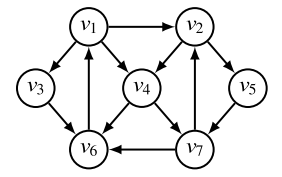
\includegraphics[width=0.4\textwidth]{Fig_1_30.png}

\textbf{Vertices}: $v_1, v_2, v_3, v_4, v_5, v_6, v_7$

\textbf{Edges in the undirected version}:
\[
\begin{aligned}
&v_1 - v_2,\quad v_1 - v_3,\quad v_1 - v_4,\quad v_2 - v_4,\quad v_2 - v_5, \quad v_1 - v_6, \\
&v_3 - v_6,\quad v_4 - v_6,\quad v_4 - v_7,\quad v_5 - v_7,\quad v_6 - v_7, \quad v_2 - v_7
\end{aligned}
\]

There are $7$ vertices and $12$ edges in the undirected version. A spanning tree of this graph will have exactly $6$ edges and no cycles.

\textbf{Solution}

Spanning tree of the graph in Fig. 1.30:
\begin{align*}
    T_1 &= \{ \{v_1 \to v_2\}, \{v_2 \to v_5\}, \{v_5 \to v_7\}, \{v_1 \to v_3\}, \{v_3 \to v_6\}, \{v_1 \to v_4\} \} \\
    T_2 &= \{ \{v_1 \to v_2\}, \{v_2 \to v_5\}, \{v_5 \to v_7\}, \{v_1 \to v_3\}, \{v_3 \to v_6\}, \{v_2 \to v_4\} \} \\
    T_3 &= \{ \{v_1 \to v_4\}, \{v_4 \to v_7\}, \{v_7 \to v_2\}, \{v_1 \to v_3\}, \{v_3 \to v_6\}, \{v_2 \to v_5\} \} \\
    T_4 &= \{ \{v_1 \to v_4\}, \{v_4 \to v_7\}, \{v_1 \to v_2\}, \{v_1 \to v_3\}, \{v_3 \to v_6\}, \{v_2 \to v_5\} \} \\
    T_5 &= \{ \{v_1 \to v_3\}, \{v_6 \to v_1\}, \{v_1 \to v_4\}, \{v_4 \to v_7\}, \{v_7 \to v_2\}, \{v_2 \to v_5\} \} \\
    T_6 &= \{ \{v_1 \to v_3\}, \{v_6 \to v_1\}, \{v_1 \to v_4\}, \{v_2 \to v_4\}, \{v_7 \to v_2\}, \{v_5 \to v_7\} \} \\
    T_7 &= \{ \{v_1 \to v_3\}, \{v_6 \to v_1\}, \{v_7 \to v_6\}, \{v_7 \to v_2\}, \{v_2 \to v_5\}, \{v_2 \to v_4\} \} \\
    T_8 &= \{ \{v_1 \to v_3\}, \{v_6 \to v_1\}, \{v_7 \to v_6\}, \{v_7 \to v_2\}, \{v_2 \to v_5\}, \{v_1 \to v_4\} \} \\
\end{align*}

\begin{verbatim}
    import networkx as nx
    
    G = nx.Graph()
    edges = [
        (1, 2), (1, 3), (1, 4),
        (2, 4), (2, 5), (3, 6),
        (4, 6), (4, 7), (5, 7), (6, 7)
    ]
    G.add_edges_from(edges)
    
    n_spanning_trees = nx.number_of_spanning_trees(G)
    print(n_spanning_trees)
\end{verbatim}

Using the code above, we can get the number of spanning trees of the underlying undirected graph in Fig. 1.30 is \textbf{288}.

\textbf{Explanation of \texttt{number\_of\_spanning\_trees()}}

The function \texttt{networkx.number\_of\_spanning\_trees(G)} returns the total number of distinct spanning trees of a connected undirected graph \( G \). 

Internally, it applies the \textbf{Matrix-Tree Theorem}, which states:

\begin{quote}
The number of spanning trees of a graph is equal to any cofactor (i.e., determinant of a minor) of its Laplacian matrix.
\end{quote}

Given a graph \( G \) with \( n \) vertices, the Laplacian matrix \( L \) is defined as:
\[
L = D - A
\]
where:
\begin{itemize}
    \item \( D \) is the degree matrix (a diagonal matrix where \( D_{ii} \) is the degree of vertex \( v_i \)),
    \item \( A \) is the adjacency matrix of the graph.
\end{itemize}

To compute the number of spanning trees, one row and the corresponding column are removed from \( L \), and the determinant of the resulting \((n-1) \times (n-1)\) matrix is taken.

This value is guaranteed to be an integer for any connected undirected graph.

\textbf{Problem 1.4}

\textbf{Extend the adjacency matrix graph representation by replacing those operations having an edge as argument or giving an edge or a list of edges as result, by corresponding operations having as argument or giving as result the source and target vertices of the edge or edges.}

\textbf{Explanation:}

In many graph libraries, edge-based operations are defined using edge objects or identifiers. However, when using an adjacency matrix representation, edges are naturally represented by ordered pairs of vertices \((v, w)\) such that the matrix entry \(A[v][w] = 1\). Therefore, we can extend and redefine these operations directly in terms of vertex pairs:

\begin{itemize}
    \item \texttt{G.del\_edge(e)} $\Rightarrow$ \texttt{G.del\_edge(v, w)} \\
    Deletes the edge from vertex \(v\) to vertex \(w\) by setting \(A[v][w] := 0\).

    \item \texttt{G.edges()} $\Rightarrow$ return all pairs \((v, w)\) such that \(A[v][w] = 1\) \\
    Returns the set of all edges as vertex pairs.

    \item \texttt{G.incoming(v)} $\Rightarrow$ return all \(u\) such that \(A[u][v] = 1\) \\
    Returns all vertices that have an edge going into vertex \(v\).

    \item \texttt{G.outgoing(v)} $\Rightarrow$ return all \(w\) such that \(A[v][w] = 1\) \\
    Returns all vertices that are targets of edges going out from vertex \(v\).

    \item \texttt{G.source(e)} $\Rightarrow$ extract \(v\) from edge \((v, w)\) \\
    The source of the edge is simply the first vertex of the pair.

    \item \texttt{G.target(e)} $\Rightarrow$ extract \(w\) from edge \((v, w)\) \\
    The target of the edge is the second vertex of the pair.
\end{itemize}

\textbf{Problem 1.5}

\textbf{Extend the first-child, next-sibling tree representation, in order to support the operations} \texttt{T.root()}, \texttt{T.number\_of\_children(v)}, \texttt{T.children(v)} \textbf{in} $\mathcal{O}(1)$ \textbf{time}.

\textbf{Solution:}

We augment the traditional first-child, next-sibling (FCNS) tree structure by storing additional information in each node and in the tree structure itself.

\begin{itemize}
    \item \texttt{T.root()}: Maintain a direct reference to the root node in the tree object \texttt{T}. Accessing the root is then a simple pointer dereference and takes constant time.

    \item \texttt{T.number\_of\_children(v)}: Add a field \texttt{v.num\_children} in each node \texttt{v}, which is incremented or decremented whenever a child is added or removed. This allows the number of children to be returned in constant time.

    \item \texttt{T.children(v)}: In addition to \texttt{v.first\_child} and \texttt{v.next\_sibling}, maintain a separate list or array \texttt{v.children[]} storing direct references to all of \texttt{v}'s children. This allows for immediate access to all children in $\mathcal{O}(1)$ time if the list is directly returned (not iterated over).
\end{itemize}

\textbf{Trade-off:}  
These enhancements increase the space complexity and require careful maintenance of the extra fields during updates (insertions, deletions). However, they provide significant performance improvements for child-related queries.

\textbf{Problem 1.6}

\textbf{Show how to double check that the graph-based representation of a tree is indeed a tree, in time linear in the size of the tree.}

To verify that a graph-based representation indeed corresponds to a valid tree, we perform the following checks in $O(n)$ time, where $n$ is the number of nodes in the graph:

\begin{enumerate}
    \item \textbf{Check for exactly one root node.}
    
    A root node is defined as a node with no incoming edges. We iterate through all nodes and count how many satisfy this condition:
    \[
    \text{root\_count} \gets 0
    \]
    \[
    \text{for each } v \in T.vertices(): \quad \text{if } T.incoming(v).empty(): \quad \text{root\_count} \gets \text{root\_count} + 1
    \]
    If $\text{root\_count} \ne 1$, the structure is not a valid tree.

    \item \textbf{Check that every non-root node has exactly one parent.}
    
    For each node $v$ with incoming edges, we ensure:
    \[
    \text{if } \neg T.incoming(v).empty(), \text{ then } T.incoming(v).size() = 1
    \]
    This guarantees that every node except the root has exactly one parent.

    \item \textbf{Check for connectivity and absence of cycles using DFS.}
    
    We perform a depth-first search (DFS) from the root node and:
    \begin{itemize}
        \item Mark each visited node to avoid revisiting.
        \item If a node is visited more than once, a cycle exists.
        \item If some nodes are not visited after DFS, the graph is disconnected.
    \end{itemize}

    \textit{Pseudocode:}
    \begin{verbatim}
visited = empty set

function DFS(v):
    if v in visited:
        return False  # cycle detected
    visited.add(v)
    for u in T.children(v):
        if not DFS(u):
            return False
    return True
    \end{verbatim}

    After DFS:
    \[
    \text{if } |\text{visited}| \ne T.number\_of\_nodes(), \text{ the structure is not connected.}
    \]
\end{enumerate}

\noindent
Since each operation (checking incoming/outgoing edges, DFS traversal) takes constant or linear time over all nodes and edges, the total verification process runs in $O(n)$ time.

\textbf{Exercise 1.1: The standard representation of an undirected graph in the format adopted for the DIMACS Implementation Challenges consists of a problem definition line of the form \texttt{p edge n m}, where $n$ and $m$ are, respectively, the number of vertices and the number of edges, followed by $m$ edge descriptor lines of the form \texttt{e i j}, each of them giving an edge as a pair of vertex numbers in the range $1$ to $n$. Comment lines of the form \texttt{c …} are also allowed. Implement procedures to read a DIMACS graph and to write a graph in DIMACS format.}

The DIMACS format represents an undirected graph in a standardized way:
\begin{itemize}
    \item Comment lines start with \texttt{c} and can be ignored.
    \item A line starting with \texttt{p edge n m} defines the number of vertices ($n$) and edges ($m$).
    \item Each subsequent line starting with \texttt{e i j} defines an undirected edge between vertex $i$ and vertex $j$.
\end{itemize}

To handle this format, we implement two procedures:

\textbf{Reading a DIMACS graph}
We read each line of the input file:
\begin{itemize}
    \item Skip lines starting with \texttt{c}.
    \item Parse the line \texttt{p edge n m} to get the number of vertices and edges.
    \item Parse each edge line \texttt{e u v} and store the edges as pairs $(u,v)$.
\end{itemize}

\textbf{Writing a DIMACS graph}
To output a graph in DIMACS format:
\begin{itemize}
    \item Print the line \texttt{p edge n m}, where $m$ is the number of edges.
    \item For each edge $(u, v)$, write the line \texttt{e u v}.
\end{itemize}

\textbf{Exercise 1.2: The external representation of a graph in the Stanford GraphBase (SGB) format consists essentially of a first line of the form \texttt{* GraphBase graph (utiltypes …,nV,mA)}, where $n$ and $m$ are, respectively, the number of vertices and the number of edges; a second line containing an identification string; a \texttt{* Vertices} line; $n$ vertex descriptor lines of the form \texttt{label,Ai,0,0}, where $i$ is the number of the first edge in the range $0$ to $m - 1$ going out of the vertex and \texttt{label} is a string label; an \texttt{* Arcs} line; $m$ edge descriptor lines of the form \texttt{V j,Ai,label,0}, where $j$ is the number of the target vertex in the range $0$ to $n - 1$, $i$ is the number of the next edge in the range $0$ to $m - 1$ going out of the same source vertex, and \texttt{label} is an integer label; and a last \texttt{* Checksum …} line. Further, in the description of a vertex with no outgoing edge, or an edge with no successor going out of the same source vertex, \texttt{Ai} becomes \texttt{0}. Implement procedures to read a SGB graph and to write a graph in SGB format.}

The \textbf{Stanford GraphBase (SGB)} format represents a directed graph in a structured way:

\begin{itemize}
    \item The first line begins with \texttt{* GraphBase graph (utiltypes ...,nV,mA)} where $n$ is the number of vertices and $m$ is the number of edges.
    \item The second line is an identification string (can be stored or ignored).
    \item The \texttt{* Vertices} section follows, with $n$ lines describing vertices in the format: \texttt{label,Ai,0,0}
    \begin{itemize}
        \item \texttt{label} is a string identifier.
        \item \texttt{Ai} indicates the index (from $0$ to $m-1$) of the first outgoing edge from that vertex.
        \item If there is no outgoing edge, \texttt{Ai} is \texttt{0}.
    \end{itemize}
    \item Then comes the \texttt{* Arcs} section, with $m$ lines describing directed edges (arcs) in the format: \texttt{Vj,Ai,label,0}
    \begin{itemize}
        \item \texttt{Vj} is the target vertex (in the range $0$ to $n-1$).
        \item \texttt{Ai} is the index of the next edge from the same source vertex.
        \item If there is no next edge, \texttt{Ai} is \texttt{0}.
        \item \texttt{label} is an integer label for the edge.
    \end{itemize}
    \item A final line \texttt{* Checksum ...} concludes the graph.
\end{itemize}

To process this format, we implement two procedures:

\textbf{Reading a SGB graph}
\begin{itemize}
    \item Parse the first line to extract $n$ and $m$.
    \item Skip or store the second line (identifier).
    \item In the \texttt{* Vertices} section:
    \begin{itemize}
        \item Read each vertex’s label and first outgoing edge index.
        \item Store vertex labels and associate them with outgoing edge indices.
    \end{itemize}
    \item In the \texttt{* Arcs} section:
    \begin{itemize}
        \item Read each edge’s target vertex, next edge index, and label.
        \item Construct an adjacency list or edge list accordingly.
    \end{itemize}
\end{itemize}

\textbf{Writing a SGB graph}
\begin{itemize}
    \item Output the graph header and identification string.
    \item Write the \texttt{* Vertices} section with vertex descriptors.
    \item Write the \texttt{* Arcs} section with edge descriptors.
    \item Append a \texttt{* Checksum ...} line if needed.
\end{itemize}

\textbf{Exercise 1.3}

\textbf{Implement algorithms to generate the path graph $P_n$, the circle graph $C_n$, and the wheel graph $W_n$ on $n$ vertices, using the collection of 32 abstract operations from Sect. 1.3.}

\textbf{Definitions}

\begin{itemize}
    \item A \textbf{path graph} $P_n$ on $n$ vertices is a graph with $n$ vertices and $n-1$ edges, forming a single path.
    \item A \textbf{circle graph} $C_n$ on $n$ vertices is a graph with $n$ vertices and $n$ edges, forming a single cycle. $C_n$ is defined for $n \ge 3$.
    \item A \textbf{wheel graph} $W_n$ on $n$ vertices is formed by connecting a single "hub" vertex to all vertices of a cycle graph $C_{n-1}$. Thus, $W_n$ has $n$ vertices and $2(n-1)$ edges. $W_n$ is defined for $n \ge 4$.
\end{itemize}

\textbf{Solution}

We will provide algorithms for generating each of the specified graph types. These algorithms assume the availability of a `Graph` object with the abstract operations listed in the problem description.

\begin{itemize}
    \item \textbf{Algorithm to Generate Path Graph $P_n$}
    
    A path graph $P_n$ is constructed by sequentially adding $n$ vertices and then connecting each vertex to its successor.
    
    \begin{itemize}
        \item \textbf{Procedure} GeneratePathGraph($n$)
        \item \hspace{0.5cm} $G \gets \text{new Graph}()$
        \item \hspace{0.5cm} \textbf{If} $n \le 1$ \textbf{Then}
        \item \hspace{1cm} \textbf{Return} $G$
        \item \hspace{0.5cm} \textbf{End If}
        \item \hspace{0.5cm} $V \gets []$ (List to store created vertices)
        \item \hspace{0.5cm} \textbf{For} $i \gets 0 \textbf{ to } n-1$ \textbf{Do}
        \item \hspace{1cm} $v \gets G.\text{new\_vertex}()$ (Create a new vertex)
        \item \hspace{1cm} $V.\text{append}(v)$ (Add vertex to our list)
        \item \hspace{0.5cm} \textbf{End For}
        \item \hspace{0.5cm} \textbf{For} $i \gets 0 \textbf{ to } n-2$ \textbf{Do}
        \item \hspace{1cm} $G.\text{new\_edge}(V[i], V[i+1])$ (Add an edge between consecutive vertices)
        \item \hspace{0.5cm} \textbf{End For}
        \item \hspace{0.5cm} \textbf{Return} $G$
        \item \textbf{End Procedure}
    \end{itemize}

    \item \textbf{Algorithm to Generate Circle Graph $C_n$}
    
    A circle graph $C_n$ builds upon the path graph structure by adding one additional edge to connect the last vertex back to the first, thereby completing the cycle. This is valid for $n \ge 3$.
    
    \begin{itemize}
        \item \textbf{Procedure} GenerateCircleGraph($n$)
        \item \hspace{0.5cm} $G \gets \text{new Graph}()$
        \item \hspace{0.5cm} \textbf{If} $n < 3$ \textbf{Then}
        \item \hspace{1cm} \textbf{Return} $G$
        \item \hspace{0.5cm} \textbf{End If}
        \item \hspace{0.5cm} $V \gets []$ (List to store created vertices)
        \item \hspace{0.5cm} \textbf{For} $i \gets 0 \textbf{ to } n-1$ \textbf{Do}
        \item \hspace{1cm} $v \gets G.\text{new\_vertex}()$
        \item \hspace{1cm} $V.\text{append}(v)$
        \item \hspace{0.5cm} \textbf{End For}
        \item \hspace{0.5cm} \textbf{For} $i \gets 0 \textbf{ to } n-2$ \textbf{Do}
        \item \hspace{1cm} $G.\text{new\_edge}(V[i], V[i+1])$ (Add edges to form a path)
        \item \hspace{0.5cm} \textbf{End For}
        \item \hspace{0.5cm} $G.\text{new\_edge}(V[n-1], V[0])$ (Add the closing edge to complete the cycle)
        \item \hspace{0.5cm} \textbf{Return} $G$
        \item \textbf{End Procedure}
    \end{itemize}

    \item \textbf{Algorithm to Generate Wheel Graph $W_n$}
    
    A wheel graph $W_n$ is formed by creating a central "hub" vertex and a cycle graph $C_{n-1}$ with the remaining $n-1$ vertices. The hub vertex is then connected to every vertex in the cycle. This is valid for $n \ge 4$.
    
    \begin{itemize}
        \item \textbf{Procedure} GenerateWheelGraph($n$)
        \item \hspace{0.5cm} $G \gets \text{new Graph}()$
        \item \hspace{0.5cm} \textbf{If} $n < 4$ \textbf{Then}
        \item \hspace{1cm} \textbf{Return} $G$
        \item \hspace{0.5cm} \textbf{End If}
        \item \hspace{0.5cm} $v_h \gets G.\text{new\_vertex}()$ (Create the central hub vertex)
        \item \hspace{0.5cm} $V_{cycle} \gets []$ (List to store vertices for the cycle)
        \item \hspace{0.5cm} \textbf{For} $i \gets 0 \textbf{ to } n-2$ \textbf{Do}
        \item \hspace{1cm} $v \gets G.\text{new\_vertex}()$ (Create a vertex for the cycle)
        \item \hspace{1cm} $V_{cycle}.\text{append}(v)$
        \item \hspace{0.5cm} \textbf{End For}
        \item \hspace{0.5cm} (Form the cycle $C_{n-1}$)
        \item \hspace{0.5cm} \textbf{For} $i \gets 0 \textbf{ to } n-3$ \textbf{Do}
        \item \hspace{1cm} $G.\text{new\_edge}(V_{cycle}[i], V_{cycle}[i+1])$ (Add edges for the path part of the cycle)
        \item \hspace{0.5cm} \textbf{End For}
        \item \hspace{0.5cm} $G.\text{new\_edge}(V_{cycle}[n-2], V_{cycle}[0])$ (Add the closing edge to complete the cycle)
        \item \hspace{0.5cm} (Add edges from the hub to all cycle vertices)
        \item \hspace{0.5cm} \textbf{For} $i \gets 0 \textbf{ to } n-2$ \textbf{Do}
        \item \hspace{1cm} $G.\text{new\_edge}(v_h, V_{cycle}[i])$ (Connect hub to each cycle vertex)
        \item \hspace{0.5cm} \textbf{End For}
        \item \hspace{0.5cm} \textbf{Return} $G$
        \item \textbf{End Procedure}
    \end{itemize}
\end{itemize}

\textbf{Exercise 1.4}

\textbf{Implement an algorithm to generate the complete graph $K_n$ on $n$ vertices and the complete bipartite graph $K_{p,q}$ with $p + q$ vertices, using the collection of 32 abstract operations from Sect. 1.3.}

\textbf{Definitions}

\begin{itemize}
    \item A \textbf{complete graph} $K_n$ is a simple undirected graph in which every pair of distinct vertices is connected by a unique edge.
    \item A \textbf{complete bipartite graph} $K_{p,q}$ is a bipartite graph whose vertex set is partitioned into two disjoint sets with $p$ and $q$ vertices respectively, and where every vertex in the first set is connected to every vertex in the second set.
\end{itemize}

\textbf{Solution}

We will provide algorithms for generating each of the specified graph types. These algorithms assume the availability of a `Graph` object with the abstract operations listed in the problem description.

\begin{itemize}
    \item \textbf{Algorithm to Generate Complete Graph $K_n$}
    
    A complete graph $K_n$ is formed by creating $n$ vertices and then adding an edge between every unique pair of these vertices.
    
    \begin{itemize}
        \item \textbf{Procedure} GenerateCompleteGraph($n$)
        \item \hspace{0.5cm} $G \gets \text{new Graph}()$
        \item \hspace{0.5cm} \textbf{If} $n \le 0$ \textbf{Then}
        \item \hspace{1cm} \textbf{Return} $G$
        \item \hspace{0.5cm} \textbf{End If}
        \item \hspace{0.5cm} $V \gets []$ (List to store created vertices)
        \item \hspace{0.5cm} \textbf{For} $i \gets 0 \textbf{ to } n-1$ \textbf{Do}
        \item \hspace{1cm} $v \gets G.\text{new\_vertex}()$ (Create a new vertex)
        \item \hspace{1cm} $V.\text{append}(v)$ (Add vertex to our list)
        \item \hspace{0.5cm} \textbf{End For}
        \item \hspace{0.5cm} (Add an edge between every distinct pair of vertices)
        \item \hspace{0.5cm} \textbf{For} $i \gets 0 \textbf{ to } n-1$ \textbf{Do}
        \item \hspace{1cm} \textbf{For} $j \gets i+1 \textbf{ to } n-1$ \textbf{Do}
        \item \hspace{1.5cm} $G.\text{new\_edge}(V[i], V[j])$
        \item \hspace{1cm} \textbf{End For}
        \item \hspace{0.5cm} \textbf{End For}
        \item \hspace{0.5cm} \textbf{Return} $G$
        \item \textbf{End Procedure}
    \end{itemize}

    \item \textbf{Algorithm to Generate Complete Bipartite Graph $K_{p,q}$}
    
    A complete bipartite graph $K_{p,q}$ is constructed by creating two disjoint sets of vertices, one with $p$ vertices and another with $q$ vertices. Then, an edge is added from every vertex in the first set to every vertex in the second set.
    
    \begin{itemize}
        \item \textbf{Procedure} GenerateCompleteBipartiteGraph($p, q$)
        \item \hspace{0.5cm} $G \gets \text{new Graph}()$
        \item \hspace{0.5cm} \textbf{If} $p < 0 \textbf{ or } q < 0$ \textbf{Then}
        \item \hspace{1cm} \textbf{Return} $G$ (Invalid input for p or q)
        \item \hspace{0.5cm} \textbf{End If}
        \item \hspace{0.5cm} $V_P \gets []$ (List to store vertices of the first set (size p))
        \item \hspace{0.5cm} $V_Q \gets []$ (List to store vertices of the second set (size q))
        \item \hspace{0.5cm} (Create p vertices for the first set)
        \item \hspace{0.5cm} \textbf{For} $i \gets 0 \textbf{ to } p-1$ \textbf{Do}
        \item \hspace{1cm} $v \gets G.\text{new\_vertex}()$
        \item \hspace{1cm} $V_P.\text{append}(v)$
        \item \hspace{0.5cm} \textbf{End For}
        \item \hspace{0.5cm} (Create q vertices for the second set)
        \item \hspace{0.5cm} \textbf{For} $i \gets 0 \textbf{ to } q-1$ \textbf{Do}
        \item \hspace{1cm} $v \gets G.\text{new\_vertex}()$
        \item \hspace{1cm} $V_Q.\text{append}(v)$
        \item \hspace{0.5cm} \textbf{End For}
        \item \hspace{0.5cm} \textbf{For each} $u \textbf{ in } V_P$ \textbf{Do}
        \item \hspace{1cm} \textbf{For each} $v \textbf{ in } V_Q$ \textbf{Do}
        \item \hspace{1.5cm} $G.\text{new\_edge}(u, v)$
        \item \hspace{1cm} \textbf{End For}
        \item \hspace{0.5cm} \textbf{End For}
        \item \hspace{0.5cm} \textbf{Return} $G$
        \item \textbf{End Procedure}
    \end{itemize}
\end{itemize}

\textbf{Exercise 1.5}

\textbf{Implement the extended adjacency matrix graph representation given in Problem 1.4, wrapped in a Python class, using Python lists together with the internal numbering of the vertices.}

\textbf{Solution}

We will implement a Python class `GraphAdjacencyMatrix` that represents a graph using an adjacency matrix. The vertices will be internally numbered from $0$ up to $n-1$. The abstract operations will be implemented, with those from Problem 1.4 adapted to use source and target vertices directly instead of edge objects.

The adjacency matrix will be a list of lists (a 2D list) where \texttt{self.adj\_matrix[u][v] = 1} if an edge exists from vertex \texttt{u} to vertex \texttt{v}, and \texttt{0} otherwise.

\begin{itemize}
    \item \textbf{Class `GraphAdjacencyMatrix` Implementation}

    \textbf{Core Data Structure:}
    \begin{itemize}
        \item \texttt{self.adj\_matrix}: A list of lists representing the adjacency matrix.
        \item \texttt{self.num\_vertices}: An integer tracking the current number of vertices.
        \item \texttt{self.num\_edges}: An integer tracking the current number of edges.
        \item \texttt{self.vertex\_map}: A list to store the actual vertex objects (or simply their internal integer IDs if vertices are just numbers). For this implementation, we'll assume vertices are represented by their integer indices.
    \end{itemize}

    \textbf{Abstract Operations Implementation:}

    \begin{itemize}
        \item \textbf{Initialization:}
        \begin{itemize}
            \item \texttt{\_\_init\_\_(self)}: Initializes an empty graph with an empty adjacency matrix, zero vertices, and zero edges.
        \end{itemize}
        
        \item \textbf{Vertex and Edge Creation/Deletion:}
        \begin{itemize}
            \item \texttt{new\_vertex(self)}: Adds a new vertex to the graph. Expands the adjacency matrix.
            \item \texttt{new\_edge(self, u, v)}: Inserts a new edge from vertex \texttt{u} to vertex \texttt{v}. Updates \texttt{self.adj\_matrix[u][v]} to \texttt{1}.
            \item \texttt{del\_vertex(self, v)}: Deletes vertex \texttt{v} and all incident edges. This involves removing the corresponding row and column from the adjacency matrix and re-indexing subsequent vertices. This is a complex operation for an adjacency matrix and typically inefficient. For simplicity in this context, we will mark vertices as "inactive" rather than physically resizing the matrix for deletion, or raise an error if re-indexing is not explicitly required. A true "delete and re-index" would require a new matrix. A simplified \texttt{del\_vertex} might just set all incoming/outgoing edges to \texttt{0} and conceptually remove the vertex.
            \item \texttt{del\_edge(self, u, v)}: Deletes the edge from vertex \texttt{u} to vertex \texttt{v}. Sets \texttt{self.adj\_matrix[u][v]} to \texttt{0}.
        \end{itemize}

        \item \textbf{Graph Information:}
        \begin{itemize}
            \item \texttt{number\_of\_vertices(self)}: Returns \texttt{self.num\_vertices}.
            \item \texttt{number\_of\_edges(self)}: Returns \texttt{self.num\_edges}.
            \item \texttt{vertices(self)}: Returns a list of all active vertex indices (0 to \texttt{num\_vertices-1}).
            \item \texttt{edges(self)}: Returns a list of all edges as \texttt{(source, target)} tuples where \texttt{self.adj\_matrix[source][target] == 1}.
            \item \texttt{adjacent(self, u, v)}: Returns \texttt{True} if \texttt{self.adj\_matrix[u][v] == 1}, \texttt{False} otherwise.
        \end{itemize}

        \item \textbf{Vertex-Specific Information (Extended for Problem 1.4):}
        \begin{itemize}
            \item \texttt{incoming(self, v)}: Returns a list of \texttt{source} vertices such that \texttt{self.adj\_matrix[source][v] == 1}.
            \item \texttt{outgoing(self, v)}: Returns a list of \texttt{target} vertices such that \texttt{self.adj\_matrix[v][target] == 1}.
            \item \texttt{indeg(self, v)}: Returns the count of incoming edges to \texttt{v}.
            \item \texttt{outdeg(self, v)}: Returns the count of outgoing edges from \texttt{v}.
        \end{itemize}

        \item \textbf{Traversal Operations (Simulated):}
        \begin{itemize}
            \item \texttt{first\_vertex(self)}: Returns the smallest active vertex index.
            \item \texttt{last\_vertex(self)}: Returns the largest active vertex index.
            \item \texttt{pred\_vertex(self, v)}: Returns \texttt{v-1} if $v > 0$.
            \item \texttt{succ\_vertex(self, v)}: Returns \texttt{v+1} if $v < \text{num\_vertices}-1$.
            \item \texttt{first\_edge(self)}: Returns the first \texttt{(u,v)} edge found by iterating through the matrix.
            \item \texttt{last\_edge(self)}: Returns the last \texttt{(u,v)} edge found.
            \item \texttt{pred\_edge(self, edge)}: Given \texttt{(u,v)}, returns the "previous" edge in row-major order. (Complex for direct adjacency matrix, will be simplified to finding the previous edge by iterating).
            \item \texttt{succ\_edge(self, edge)}: Given \texttt{(u,v)}, returns the "next" edge. (Complex for direct adjacency matrix, will be simplified).
            \item \texttt{first\_in\_edge(self, v)}: Returns the first \texttt{(u,v)} edge incoming to \texttt{v}.
            \item \texttt{last\_in\_edge(self, v)}: Returns the last \texttt{(u,v)} edge incoming to \texttt{v}.
            \item \texttt{in\_pred(self, edge)}: Returns the previous incoming edge for \texttt{edge[1]}.
            \item \texttt{in\_succ(self, edge)}: Returns the next incoming edge for \texttt{edge[1]}.
            \item \texttt{first\_adj\_edge(self, v)}: Returns the first \texttt{(v,w)} edge outgoing from \texttt{v}.
            \item \texttt{last\_adj\_edge(self, v)}: Returns the last \texttt{(v,w)} edge outgoing from \texttt{v}.
            \item \texttt{adj\_pred(self, edge)}: Returns the previous outgoing edge for \texttt{edge[0]}.
            \item \texttt{adj\_succ(self, edge)}: Returns the next outgoing edge for \texttt{edge[0]}.
        \end{itemize}
        
        \item \textbf{Edge Source/Target (Problem 1.4 Specific):}
        \begin{itemize}
            \item \texttt{source(self, edge)}: Returns \texttt{edge[0]}.
            \item \texttt{target(self, edge)}: Returns \texttt{edge[1]}.
            \item \texttt{opposite(self, v, edge)}: Returns \texttt{edge[1]} if \texttt{v == edge[0]}, else \texttt{edge[0]}.
        \end{itemize}
    \end{itemize}
\end{itemize}

\textbf{Exercise 1.6}

\textbf{Enumerate all perfect matchings in the complete bipartite graph $K_{p,q}$ on $p + q$ vertices.}

\textbf{Definitions}

\begin{itemize}
    \item A \textbf{bipartite graph} is a graph whose vertices can be divided into two disjoint and independent sets, $L$ and $R$, such that every edge connects a vertex in $L$ to one in $R$.
    \item A \textbf{complete bipartite graph} $K_{p,q}$ is a bipartite graph where the two sets of vertices have sizes $p$ and $q$ respectively, and every vertex in the first set is connected to every vertex in the second set.
    \item A \textbf{matching} in a graph is a set of edges such that no two edges share a common vertex.
    \item A \textbf{perfect matching} is a matching that covers all vertices in the graph. In a bipartite graph with bipartition $(L, R)$, a perfect matching exists only if $|L| = |R|$. If it exists, it will contain $|L|$ (or $|R|$) edges.
\end{itemize}

\textbf{Solution}

For a perfect matching to exist in a complete bipartite graph $K_{p,q}$, the number of vertices in both partitions must be equal, i.e., $p = q$. If $p \neq q$, there are no perfect matchings.

When $p = q = n$, the graph is $K_{n,n}$. A perfect matching in $K_{n,n}$ consists of $n$ edges, where each vertex from the first partition is paired with a unique vertex from the second partition. This problem is equivalent to finding all possible bijections (or permutations) between the vertices of the two partitions. The number of such matchings is $n!$.

We can enumerate these matchings using a recursive backtracking algorithm. Let the vertices in the first partition be $L = \{0, 1, \dots, n-1\}$ and the vertices in the second partition be $R = \{n, n+1, \dots, 2n-1\}$.

\begin{itemize}
    \item \textbf{Algorithm to Enumerate Perfect Matchings in $K_{p,q}$}

    \begin{itemize}
        \item \textbf{Procedure} EnumeratePerfectMatchingsKpq($p, q$)
        \item \hspace{0.5cm} \textbf{If} $p \neq q$ \textbf{Then}
        \item \hspace{1cm} \textbf{Return} empty list (No perfect matching exists)
        \item \hspace{0.5cm} \textbf{End If}
        \item \hspace{0.5cm} $n \gets p$
        \item \hspace{0.5cm} $all\_matchings \gets []$ (List to store all found perfect matchings)
        \item \hspace{0.5cm} $current\_matching \gets []$ (Stores edges for the current matching being built)
        \item \hspace{0.5cm} $used\_right\_vertices \gets \text{list of } n \text{ False values}$ (Boolean array to track used vertices in $R$)
        
        \item \hspace{0.5cm} \textbf{Function} FindMatchingsRecursive($l\_idx$)
        \item \hspace{1cm} \textbf{If} $l\_idx = n$ \textbf{Then}
        \item \hspace{1.5cm} Add a copy of $current\_matching$ to $all\_matchings$
        \item \hspace{1.5cm} \textbf{Return}
        \item \hspace{1cm} \textbf{End If}
        
        \item \hspace{1cm} (Iterate through all vertices in $R$ to find a match for $L[l\_idx]$)
        \item \hspace{1cm} \textbf{For} $r\_relative\_idx \gets 0 \textbf{ to } n-1$ \textbf{Do}
        \item \hspace{1.5cm} \textbf{If not} $used\_right\_vertices[r\_relative\_idx]$ \textbf{Then}
        \item \hspace{2cm} $used\_right\_vertices[r\_relative\_idx] \gets \text{True}$
        \item \hspace{2cm} $edge \gets (l\_idx, n + r\_relative\_idx)$ (Form edge using absolute vertex IDs)
        \item \hspace{2cm} Add $edge$ to $current\_matching$
        \item \hspace{2cm} Call FindMatchingsRecursive($l\_idx + 1$)
        \item \hspace{2cm} (Backtrack: undo the choice for the current $L[l\_idx]$)
        \item \hspace{2cm} Remove last edge from $current\_matching$
        \item \hspace{2cm} $used\_right\_vertices[r\_relative\_idx] \gets \text{False}$
        \item \hspace{1.5cm} \textbf{End If}
        \item \hspace{1cm} \textbf{End For}
        \item \hspace{0.5cm} \textbf{End Function}
        
        \item \hspace{0.5cm} Call FindMatchingsRecursive($0$) (Start matching from the first vertex in $L$)
        \item \hspace{0.5cm} \textbf{Return} $all\_matchings$
    \end{itemize}
\end{itemize}

\textbf{Exercise 1.7}

\textbf{Implement an algorithm to generate the complete binary tree with $n$ nodes, using the collection of 13 abstract operations from Sect. 1.3.}

\textbf{Definitions}

\begin{itemize}
    \item A \textbf{binary tree} is a tree in which each node has at most two children, typically referred to as the left child and the right child.
    \item A \textbf{complete binary tree} is a binary tree in which every level, except possibly the last, is completely filled, and all nodes in the last level are as far left as possible.
\end{itemize}

\textbf{Assumptions for Abstract Operations (Sect. 1.3 adapted for Tree Generation):}

To generate a tree using these abstract operations, we assume the existence of a \texttt{Tree} object with methods to create and link nodes. Since the provided operations are primarily for querying tree structure, we must infer or define basic node creation and parent-child linking for the purpose of \textit{building} the tree. We will assume the following simplified core operations are available for generation:
\begin{itemize}
    \item \texttt{T.new\_node()}: Creates a new, unattached node and returns its identifier.
    \item \texttt{T.set\_root(node)}: Sets the given node as the root of the tree.
    \item \texttt{T.add\_child(parent\_node, child\_node, position)}: Adds \texttt{child\_node} as a child of \texttt{parent\_node}. \texttt{position} could be 'left' or 'right' for binary trees, or an index for ordered children. For complete binary trees, we primarily care about adding the \textit{next available} child.
    \item \texttt{T.number\_of\_nodes()}: As given.
    \item \texttt{T.root()}: As given.
    \item \texttt{T.number\_of\_children(v)}: As given.
\end{itemize}
The operations like \texttt{T.parent(v)} and \texttt{T.children(v)} implicitly define the tree structure after \texttt{add\_child} is used.

\textbf{Algorithm to Generate a Complete Binary Tree with $n$ Nodes}

A complete binary tree can be constructed level by level using a breadth-first approach. We will use a queue to keep track of parent nodes that still have available "slots" for children (i.e., less than two children).

\begin{itemize}
    \item \textbf{Procedure} GenerateCompleteBinaryTree($n$)
    \item \hspace{0.5cm} Initialize an empty Tree object, $T$.
    \item \hspace{0.5cm} \textbf{If} $n \le 0$ \textbf{Then}
    \item \hspace{1cm} Return $T$
    \item \hspace{0.5cm} \textbf{End If}
    
    \item \hspace{0.5cm} $root\_node \gets T.\text{new\_node()}$
    \item \hspace{0.5cm} $T.\text{set\_root}(root\_node)$
    \item \hspace{0.5cm} $nodes\_created \gets 1$
    \item \hspace{0.5cm} $queue \gets \text{empty Queue}$
    \item \hspace{0.5cm} $queue.\text{enqueue}(root\_node)$
    
    \item \hspace{0.5cm} \textbf{While} $nodes\_created < n$ \textbf{Do}
    \item \hspace{1cm} $current\_parent \gets queue.\text{dequeue()}$
        
    \item \hspace{1cm} Add left child if needed
    \item \hspace{1cm} \textbf{If} $nodes\_created < n$ \textbf{Then}
    \item \hspace{1.5cm} $left\_child \gets T.\text{new\_node()}$
    \item \hspace{1.5cm} $T.\text{add\_child}(current\_parent, left\_child, \text{'left'})$
    \item \hspace{1.5cm} $nodes\_created \gets nodes\_created + 1$
    \item \hspace{1.5cm} $queue.\text{enqueue}(left\_child)$
    \item \hspace{1cm} \textbf{End If}
        
    \item \hspace{1cm} Add right child if needed
    \item \hspace{1cm} \textbf{If} $nodes\_created < n$ \textbf{Then}
    \item \hspace{1.5cm} $right\_child \gets T.\text{new\_node()}$
    \item \hspace{1.5cm} $T.\text{add\_child}(current\_parent, right\_child, \text{'right'})$
    \item \hspace{1.5cm} $nodes\_created \gets nodes\_created + 1$
    \item \hspace{1.5cm} $queue.\text{enqueue}(right\_child)$
    \item \hspace{1cm} \textbf{End If}
    \item \hspace{0.5cm} \textbf{End While}
    
    \item \hspace{0.5cm} \textbf{Return} $T$
    \item \textbf{End Procedure}
\end{itemize}

\textbf{Exercise 1.8}

\textbf{Implement an algorithm to generate random trees with $n$ nodes, using the collection of 13 abstract operations from Sect. 1.3. Give the time and space complexity of the algorithm.}

\textbf{Definitions}

\begin{itemize}
    \item A \textbf{tree} is an undirected graph in which any two vertices are connected by exactly one path, or equivalently, a connected acyclic graph. In the context of the abstract operations, it implies a rooted tree with parent-child relationships.
    \item A \textbf{random tree} refers to a tree generated through a stochastic process. For this exercise, we will implement a common method: generating a random tree by iteratively adding nodes and attaching each new node to a randomly selected existing node in the growing tree. This process ensures the resulting structure is always a tree.
\end{itemize}

\textbf{Assumptions for Abstract Operations (Sect. 1.3 adapted for Tree Generation):}

The 13 abstract operations provided in Section 1.3 are primarily for querying properties of an existing tree structure. To generate a tree, we must assume the availability of fundamental construction operations. We will assume the following simplified core operations for building the tree:

\begin{itemize}
    \item \texttt{T.new\_node()}: Creates a new, unattached node and returns its unique identifier. This operation is assumed to handle internal node instantiation.
    \item \texttt{T.set\_root(node)}: Sets the given \texttt{node} as the root of the tree \texttt{T}. This operation should only be called once for an empty tree.
    \item \texttt{T.add\_child(parent\_node, child\_node)}: Establishes a parent-child relationship where \texttt{child\_node} becomes a child of \texttt{parent\_node}. This operation implicitly updates the tree's internal representation such that \texttt{T.parent(child\_node)} returns \texttt{parent\_node} and \texttt{T.children(parent\_node)} includes \texttt{child\_node}.
\end{itemize}
The other 13 operations from Section 1.3 are available for querying the tree structure but are not directly used in the construction logic, other than the implicit effect of \texttt{add\_child} on them.

\textbf{Algorithm to Generate a Random Tree with $n$ Nodes}

The algorithm will start with a single root node and then iteratively add $n-1$ new nodes. Each new node will be connected as a child to a randomly chosen existing node in the tree. This ensures that the graph remains connected and acyclic throughout the process, thus forming a tree.

\begin{itemize}
    \item \textbf{Procedure} GenerateRandomTree($n$)
    \item \hspace{0.5cm} Initialize an empty Tree object, $T$.
    \item \hspace{0.5cm} Initialize an empty list, $existing\_nodes\_in\_T$.
    
    \item \hspace{0.5cm} \textbf{If} $n \le 0$ \textbf{Then}
    \item \hspace{1cm} Return $T$
    \item \hspace{0.5cm} \textbf{End If}
    
    \item \hspace{0.5cm} $root\_node \gets T.\text{new\_node()}$
    \item \hspace{0.5cm} $T.\text{set\_root}(root\_node)$
    \item \hspace{0.5cm} Add $root\_node$ to $existing\_nodes\_in\_T$.
    
    \item \hspace{0.5cm} \textbf{For} $i \gets 2 \textbf{ to } n$ \textbf{Do}
    \item \hspace{1cm} $new\_node \gets T.\text{new\_node()}$
    \item \hspace{1cm} Randomly select $parent\_candidate$ from $existing\_nodes\_in\_T$.
    \item \hspace{1cm} $T.\text{add\_child}(parent\_candidate, new\_node)$
    \item \hspace{1cm} Add $new\_node$ to $existing\_nodes\_in\_T$.
    \item \hspace{0.5cm} \textbf{End For}
    
    \item \hspace{0.5cm} \textbf{Return} $T$
    \item \textbf{End Procedure}
\end{itemize}

\textbf{Time and Space Complexity Analysis}

Let $n$ be the number of nodes in the tree to be generated.

\begin{itemize}
    \item \textbf{Time Complexity:}
    \begin{itemize}
        \item \textbf{Initialization:} Creating an empty tree and an empty list takes constant time, $O(1)$.
        \item \textbf{Root Creation:} \texttt{T.new\_node()} and \texttt{T.set\_root()} are assumed to be $O(1)$ operations. Adding the root to $existing\_nodes\_in\_T$ (a list) is $O(1)$.
        \item \textbf{Loop for $n-1$ nodes:} The loop runs $n-1$ times.
        \begin{itemize}
            \item \texttt{T.new\_node()}: Each call is $O(1)$. Total: $O(n)$.
            \item \textbf{Randomly select parent:} If $existing\_nodes\_in\_T$ is stored in a dynamic array (like a Python list or C++ \texttt{std::vector}), selecting a random element by index is $O(1)$. Total: $O(n)$.
            \item \texttt{T.add\_child(parent\_candidate, new\_node)}: This operation's complexity depends on the underlying representation of children.
                \begin{itemize}
                    \item If children are stored in an unordered list/array within each parent, adding a child is typically $O(1)$ amortized (for dynamic arrays) or $O(1)$ (for linked lists).
                    \item If children are ordered and insertion requires shifting, it could be $O(k)$ where $k$ is the number of children, worst case $O(n)$. However, for general random tree generation, we usually assume a simple append.
                \end{itemize}
                Assuming an efficient $O(1)$ amortized \texttt{add\_child} operation: Total: $O(n)$.
            \item \textbf{Add \texttt{new\_node} to \texttt{existing\_nodes\_in\_T}:} Appending to a dynamic array is $O(1)$ amortized. Total: $O(n)$.
        \end{itemize}
        \item \textbf{Overall Time Complexity:} Summing these up, the dominant factor is the loop that runs $n-1$ times, with each iteration performing constant time operations. Therefore, the total time complexity is $O(n)$.
    \end{itemize}

    \item \textbf{Space Complexity:}
    \begin{itemize}
        \item \textbf{Tree Representation:} The tree itself will store $n$ nodes and $n-1$ edges. The internal representation (e.g., adjacency lists or parent pointers) will require space proportional to the number of nodes and edges. For an adjacency list representation where each node stores a list of its children, this would be $O(n)$ for nodes and $O(n)$ for edges, totaling $O(n)$.
        \item \textbf{Auxiliary Storage (\texttt{existing\_nodes\_in\_T}):} This list stores references to all nodes created so far. Its size grows linearly with $n$, reaching $n$ elements. This requires $O(n)$ space.
        \item \textbf{Overall Space Complexity:} The total space complexity is dominated by the tree structure and the auxiliary list, both of which are linear in $n$. Therefore, the total space complexity is $O(n)$.
    \end{itemize}
\end{itemize}

\textbf{Exercise 1.9}

\textbf{Give an implementation of operation \texttt{T.previous\_sibling(v)} using the array-of-parents tree representation.}

\textbf{Array-of-Parents Tree Representation}

In an array-of-parents tree representation, the tree structure is stored using an array (or list) where each element at index $i$ stores the parent of the node identified by index $i$.
\begin{itemize}
    \item Let the nodes be identified by integer indices from $0$ to $N-1$, where $N$ is the total number of nodes.
    \item We define an array, say \texttt{parent\_array}, of size $N$.
    \item For each node $v$ (at index $v$), \texttt{parent\_array[v]} stores the index of its parent.
    \item The root node typically has a special value in its entry, such as $-1$ or \texttt{nil}, to indicate it has no parent.
\end{itemize}
This representation directly supports the \texttt{T.parent(v)} operation by a simple array lookup.

\textbf{Abstract Operations from Sect. 1.3 relevant for \texttt{T.previous\_sibling(v)}}

To implement \texttt{T.previous\_sibling(v)} using this representation and the abstract operations, we will primarily rely on:
\begin{itemize}
    \item \texttt{T.parent(v)}: Returns the parent of node \texttt{v}. This is directly available from our \texttt{parent\_array}.
    \item \texttt{T.children(v)}: Returns a list of the children of node \texttt{v}. This operation is crucial because siblings are children of the same parent. To implement this using \texttt{parent\_array}, one would iterate through \texttt{parent\_array} and collect all nodes whose parent is \texttt{v}.
    \item The understanding that the children returned by \texttt{T.children(v)} are in a specific order fixed by the representation (e.g., by their node ID, or insertion order). For \texttt{previous\_sibling} to be well-defined, this order is essential.
\end{itemize}

\textbf{Implementation of \texttt{T.previous\_sibling(v)}}

The operation \texttt{T.previous\_sibling(v)} returns the sibling node that precedes \texttt{v} in the ordered list of children of its parent. If \texttt{v} is the root, or if \texttt{v} is the first child of its parent, it has no previous sibling, and \texttt{nil} (or an equivalent indicator like a special node ID) should be returned.

\begin{itemize}
    \item \textbf{Procedure} T.previous\_sibling($v$)
    \item \hspace{0.5cm} \textbf{If} $T.\text{is\_root}(v)$ \textbf{Then}
    \item \hspace{1cm} Return \texttt{nil} (Root has no siblings)
    \item \hspace{0.5cm} \textbf{End If}
    
    \item \hspace{0.5cm} $p \gets T.\text{parent}(v)$
    \item \hspace{0.5cm} $children\_of\_p \gets T.\text{children}(p)$ (This list must preserve the order of children)
    
    \item \hspace{0.5cm} $v\_index\_in\_children \gets \text{index of } v \text{ in } children\_of\_p$
    
    \item \hspace{0.5cm} \textbf{If} $v\_index\_in\_children > 0$ \textbf{Then}
    \item \hspace{1cm} Return $children\_of\_p[v\_index\_in\_children - 1]$
    \item \hspace{0.5cm} \textbf{Else} (v is the first child)
    \item \hspace{1cm} Return \texttt{nil}
    \item \hspace{0.5cm} \textbf{End If}
    \item \textbf{End Procedure}
\end{itemize}
\textbf{Note on T.children(p) implementation in Array-of-Parents:}
For the \texttt{T.children(p)} operation itself to be efficient with an array-of-parents, it would typically involve iterating through the entire \texttt{parent\_array} ($O(N)$ time, where $N$ is the total number of nodes) to find all nodes whose parent is $p$. Alternatively, a more augmented array-of-parents representation might include a list of children for each node, which would effectively make it an adjacency list representation. Assuming \texttt{T.children(p)} returns an ordered list, the complexity is dominated by that operation.

\textbf{Exercise 1.10}

\textbf{Implement the extended first-child, next-sibling tree representation of Problem 1.5, wrapped in a Python class, using Python lists together with the internal numbering of the nodes.}

The traditional first-child, next-sibling (FCNS) representation stores for each node:
\begin{itemize}
    \item A reference to its first child.
    \item A reference to its next sibling.
\end{itemize}
To support operations like \texttt{T.root()}, \texttt{T.number\_of\_children(v)}, and \texttt{T.children(v)} in $\mathcal{O}(1)$ time, Problem 1.5 proposed augmenting this representation. For an implementation using internal node numbering (i.e., integer IDs for nodes), this translates to maintaining several parallel lists (arrays).

\textbf{Data Structures for the Extended FCNS Representation}

We will represent nodes by their integer indices, starting from $0$. The tree state will be managed by a collection of Python lists, where the index in each list corresponds to the node ID.
\begin{itemize}
    \item \texttt{\_root}: An integer storing the ID of the tree's root node. Initialized to a sentinel value (e.g., -1) for an empty tree.
    \item \texttt{\_next\_node\_id}: An integer that keeps track of the next available unique ID for a new node.
    \item \texttt{\_parent}: A list where \texttt{\_parent[i]} stores the integer ID of the parent of node $i$. The root's parent is -1.
    \item \texttt{\_first\_child}: A list where \texttt{\_first\_child[i]} stores the integer ID of the first child of node $i$. If node $i$ has no children, this is -1.
    \item \texttt{\_next\_sibling}: A list where \texttt{\_next\_sibling[i]} stores the integer ID of the next sibling of node $i$. If node $i$ is the last child, this is -1.
    \item \texttt{\_previous\_sibling}: A list where \texttt{\_previous\_sibling[i]} stores the integer ID of the previous sibling of node $i$. This is included for $\mathcal{O}(1)$ access for \texttt{previous\_sibling(v)}. If node $i$ is the first child or has no parent, this is -1.
    \item \texttt{\_num\_children}: A list where \texttt{\_num\_children[i]} stores the integer count of children of node $i$. This is updated when children are added or removed.
    \item \texttt{\_children\_lists}: A list of lists, where \texttt{\_children\_lists[i]} is a Python list containing the integer IDs of all children of node $i$, in order. This allows for $\mathcal{O}(1)$ access to the full list of children (by returning a reference to it).
\end{itemize}
All these lists are dynamically sized using Python's list capabilities, expanding as new nodes are added. Unused slots or non-existent relationships are marked with a sentinel value (e.g., -1).

\textbf{Implementation Details and Abstract Operations}

The Python class \texttt{ExtendedFCNS\_Tree} will encapsulate these data structures and provide methods corresponding to the abstract operations from Section 1.3, along with necessary construction operations (\texttt{new\_node}, \texttt{add\_child}, \texttt{set\_root}).

\begin{itemize}
    \item \textbf{Constructor (\texttt{\_\_init\_\_})}
    \begin{itemize}
        \item Initializes all internal lists (\texttt{\_parent}, \texttt{\_first\_child}, \texttt{\_next\_sibling}, \texttt{\_previous\_sibling}, \texttt{\_num\_children}, \texttt{\_children\_lists}) as empty lists.
        \item Sets \texttt{\_root = -1} and \texttt{\_next\_node\_id = 0}.
    \end{itemize}

    \item \textbf{Node Creation (\texttt{new\_node()})}
    \begin{itemize}
        \item Assigns the current \texttt{\_next\_node\_id} as the new node's ID.
        \item Extends all internal lists by one element, initializing the new slots with sentinel values (-1 for IDs, 0 for child count, empty list for \texttt{\_children\_lists}).
        \item Increments \texttt{\_next\_node\_id}.
        \item Returns the new node's ID.
    \end{itemize}

    \item \textbf{Setting Root (\texttt{set\_root(node\_id)})}
    \begin{itemize}
        \item Sets \texttt{\_root = node\_id}.
        \item The parent of the root node is set to -1.
    \end{itemize}

    \item \textbf{Adding Child (\texttt{add\_child(parent\_id, child\_id)})}
    \begin{itemize}
        \item Sets the parent pointer for the child: \texttt{\_parent[child\_id] = parent\_id}.
        \item Increments the parent's child count: \texttt{\_num\_children[parent\_id]}.
        \item Appends \texttt{child\_id} to the parent's \texttt{\_children\_lists[parent\_id]} (this maintains the order of children).
        \item If this is the parent's first child, sets \texttt{\_first\_child[parent\_id] = child\_id}.
        \item Otherwise (if the parent already had children), finds the previously last child in \texttt{\_children\_lists[parent\_id]} and updates its \texttt{\_next\_sibling} pointer to the new \texttt{child\_id}. Also, sets the new \texttt{child\_id}'s \texttt{\_previous\_sibling} to the previously last child.
        \item This ensures all relevant pointers and counts in the extended FCNS are consistent.
    \end{itemize}

    \item \textbf{Abstract Operations Implementation:}
    \begin{itemize}
        \item \texttt{T.number\_of\_nodes()}: Returns \texttt{\_next\_node\_id}. ($\mathcal{O}(1)$)
        \item \texttt{T.root()}: Returns \texttt{\_root}. ($\mathcal{O}(1)$)
        \item \texttt{T.is\_root(v)}: Returns \texttt{v == \_root}. ($\mathcal{O}(1)$)
        \item \texttt{T.number\_of\_children(v)}: Returns \texttt{\_num\_children[v]}. ($\mathcal{O}(1)$)
        \item \texttt{T.parent(v)}: Returns \texttt{\_parent[v]}. ($\mathcal{O}(1)$)
        \item \texttt{T.children(v)}: Returns \texttt{\_children\_lists[v]}. ($\mathcal{O}(1)$)
        \item \texttt{T.is\_leaf(v)}: Returns \texttt{\_num\_children[v] == 0}. ($\mathcal{O}(1)$)
        \item \texttt{T.first\_child(v)}: Returns \texttt{\_first\_child[v]}. ($\mathcal{O}(1)$)
        \item \texttt{T.last\_child(v)}: Returns the last element of \texttt{\_children\_lists[v]} (if it exists), or -1 if no children. ($\mathcal{O}(1)$)
        \item \texttt{T.previous\_sibling(v)}: Returns \texttt{\_previous\_sibling[v]}. ($\mathcal{O}(1)$)
        \item \texttt{T.next\_sibling(v)}: Returns \texttt{\_next\_sibling[v]}. ($\mathcal{O}(1)$)
        \item \texttt{T.is\_first\_child(v)}: Returns \texttt{\_parent[v] != -1} and \texttt{\_first\_child[\_parent[v]] == v}. ($\mathcal{O}(1)$)
        \item \texttt{T.is\_last\_child(v)}: Returns \texttt{\_next\_sibling[v] == -1} and \texttt{\_parent[v] != -1}. ($\mathcal{O}(1)$)
    \end{itemize}
\end{itemize}

\begin{baitoan}[Tree edit distance]
    Viết chương trình {\sf C{\tt/}C++, Python} để giải bài toán tree edit distance problem bằng cách sử dụng: (a) Backtracking. (b) Branch-\&-bound. (c) Divide-\&-conquer -- chia để trị. (d) Dynamic programming -- Quy hoạch động.
\end{baitoan}

%------------------- Giải thích thuật toán Tree Edit Distance (Backtracking) -------------------%
\textbf{(a) Phương pháp Backtracking}

\textbf{Giải thích và công thức:}

\begin{itemize}
    \item \textbf{Bài toán Khoảng cách chỉnh sửa cây (Tree Edit Distance):}
    \begin{itemize}
        \item Cho hai cây có thứ tự $T_1$ và $T_2$.
        \item Mục tiêu là tìm một chuỗi các phép biến đổi có chi phí tối thiểu để biến $T_1$ thành $T_2$.
        \item Các phép biến đổi cơ bản:
            \begin{itemize}
                \item \textbf{Deletion (Xóa):} Xóa một nút khỏi $T_1$. Chi phí: $DEL\_COST = 1$.
                \item \textbf{Insertion (Chèn):} Chèn một nút vào $T_2$ (nút này không có nút tương ứng trong $T_1$). Chi phí: $INS\_COST = 1$.
                \item \textbf{Relabeling (Đổi nhãn):} Đổi nhãn của một nút trong $T_1$ để khớp với nhãn của nút tương ứng trong $T_2$. Chi phí: $REP\_COST = 1$.
            \end{itemize}
    \end{itemize}

    \item \textbf{Backtracking (Quay lui):}
    \begin{itemize}
        \item Backtracking là một kỹ thuật thuật toán tổng quát để tìm tất cả các giải pháp cho một vấn đề tính toán bằng cách xây dựng dần các giải pháp và loại bỏ các giải pháp không hợp lệ.
        \item Nếu một giải pháp cục bộ không thể được mở rộng thành một giải pháp hợp lệ hoàn chỉnh, thuật toán sẽ "quay lui" (backtrack) và thử một lựa chọn khác.
    \end{itemize}

    \item \textbf{Áp dụng Backtracking cho Tree Edit Distance:}
    \begin{itemize}
        \item \textbf{Ánh xạ (Mapping):} Một giải pháp cho bài toán được định nghĩa bởi một ánh xạ $M \subseteq V_1 \times V_2$ giữa các nút của $T_1$ và $T_2$. Mỗi nút $v \in V_1$ được ánh xạ tới một nút $w \in V_2$ hoặc tới một nút "ảo" $\lambda$ (ký hiệu cho việc xóa nút $v$).
        \item \textbf{Các ràng buộc (Constraints):} Ánh xạ $M$ phải thỏa mãn ba ràng buộc chính để đại diện cho một phép biến đổi cây hợp lệ:
            \begin{enumerate}
                \item \textbf{Song ánh (Bijection):} Mỗi nút trong $T_1$ được ánh xạ tới nhiều nhất một nút trong $T_2$, và mỗi nút trong $T_2$ được ánh xạ từ nhiều nhất một nút trong $T_1$.
                \item \textbf{Bảo toàn quan hệ cha-con (Parent-Child Preservation):} Nếu nút $v \in T_1$ ánh xạ tới $w \in T_2$, và $v_c$ là con của $v$, thì $v_c$ phải ánh xạ tới $w_c$ là con của $w$ (hoặc $v_c$ bị xóa).
                \item \textbf{Bảo toàn thứ tự anh em (Sibling Order Preservation):} Nếu nút $v \in T_1$ ánh xạ tới $w \in T_2$, và $v_s$ là anh/chị em đứng bên phải của $v$, thì $v_s$ phải ánh xạ tới $w_s$ là anh/chị em đứng bên phải của $w$ (hoặc $v_s$ bị xóa).
            \end{enumerate}
        \item \textbf{Ý tưởng đệ quy:}
            \begin{itemize}
                \item Duyệt qua các nút của $T_1$ theo thứ tự preorder.
                \item Tại mỗi nút $v$ của $T_1$, thử ánh xạ nó tới tất cả các nút $w \in T_2$ hợp lệ (và $\lambda$).
                \item Sau mỗi lần thử ánh xạ $(v \to w)$, cập nhật tập hợp các ứng viên hợp lệ cho các nút còn lại của $T_1$ dựa trên các ràng buộc trên.
                \item Đệ quy gọi hàm cho nút tiếp theo trong preorder.
                \item Nếu tất cả các nút của $T_1$ đã được ánh xạ, một giải pháp hoàn chỉnh được tìm thấy, tính toán chi phí và lưu trữ.
                \item Sau khi nhánh đệ quy kết thúc, quay lui để thử các ánh xạ khác.
            \end{itemize}
    \end{itemize}
\end{itemize}

\textbf{Giải thích code:}

\begin{itemize}
    \item \textbf{Các hằng số và chi phí:}
    \begin{itemize}
        \item \texttt{LAMBDA\_NODE = -1}: Biến số nguyên đặc biệt đại diện cho nút "ảo" $\lambda$ (nút bị xóa). Giá trị này được chọn để không trùng với bất kỳ ID nút hợp lệ nào (ID nút bắt đầu từ 0).
        \item \texttt{DEL\_COST}, \texttt{INS\_COST}, \texttt{REP\_COST}: Chi phí cho các phép biến đổi tương ứng.
    \end{itemize}

    \item \textbf{Các lớp và cấu trúc dữ liệu:}
    \begin{itemize}
        \item \texttt{struct TreeNode}: Biểu diễn một nút của cây với các thuộc tính như ID, nhãn, ID cha, danh sách con, độ sâu, và chỉ số thứ tự duyệt preorder.
        \item \texttt{class Tree}: Biểu diễn một cây có thứ tự.
            \begin{itemize}
                \item \texttt{nodes}: Một \texttt{std::map<int, TreeNode>} lưu trữ tất cả các nút của cây, ánh xạ ID nút tới đối tượng \texttt{TreeNode}.
                \item \texttt{root\_id}: ID của nút gốc.
                \item \texttt{add\_node(...)}: Thêm một nút mới vào cây.
                \item \texttt{get\_node(...)}: Trả về con trỏ tới nút theo ID (hoặc \texttt{nullptr} nếu không tìm thấy).
                \item \texttt{compute\_preorder\_and\_depth()}: Thực hiện duyệt DFS để tính toán độ sâu và chỉ số preorder cho tất cả các nút, lưu vào \texttt{\_preorder\_traversal\_list}.
            \end{itemize}
        \item \texttt{struct Solution}: Lưu trữ một giải pháp tìm được, bao gồm ánh xạ (\texttt{mapping}), tổng chi phí (\texttt{cost}), và chi tiết về số lượng xóa, chèn, đổi nhãn (\texttt{details}).
    \end{itemize}

    \item \textbf{Các hàm chính:}
    \begin{itemize}
        \item \texttt{calculate\_edit\_distance(T1, T2, M)}:
            \begin{itemize}
                \item Tham số: Hai cây $T_1, T_2$ và một ánh xạ $M$ hoàn chỉnh.
                \item Chức năng: Tính toán tổng chi phí (xóa, chèn, đổi nhãn) cho ánh xạ $M$ đã cho.
                \item Cách tính:
                    \begin{itemize}
                        \item \textbf{Xóa:} Duyệt qua $M$, đếm số nút $v \in T_1$ được ánh xạ tới \texttt{LAMBDA\_NODE}.
                        \item \textbf{Chèn:} Đếm số nút $w \in T_2$ không được ánh xạ từ bất kỳ nút nào trong $T_1$.
                        \item \textbf{Đổi nhãn:} Duyệt qua $M$, đếm số cặp $(v, w)$ nơi $v \in T_1$ ánh xạ tới $w \in T_2$ (không phải $\lambda$) nhưng nhãn của $v$ khác nhãn của $w$.
                    \end{itemize}
            \end{itemize}
        \item \texttt{set\_up\_candidate\_nodes(T1, T2)}:
            \begin{itemize}
                \item Chức năng: Khởi tạo tập hợp ứng viên $C$. Ban đầu, với mỗi nút $v \in T_1$, $C[v]$ chứa \texttt{LAMBDA\_NODE} và tất cả các nút $w \in T_2$ có cùng độ sâu với $v$.
            \end{itemize}
        \item \texttt{refine\_candidate\_nodes(T1, T2, C\_copy, v\_id, w\_id)}:
            \begin{itemize}
                \item Chức năng: Lọc bỏ các ứng viên không hợp lệ trong $C\_copy$ dựa trên ánh xạ hiện tại $(v\_id \to w\_id)$ và các ràng buộc (song ánh, cha-con, thứ tự anh em). Hàm này thay đổi trực tiếp $C\_copy$.
            \end{itemize}
        \item \texttt{extend\_tree\_edit(T1, T2, M\_current, L\_solutions, C\_current, current\_v\_idx)}:
            \begin{itemize}
                \item Đây là hàm đệ quy cốt lõi của thuật toán backtracking.
                \item \texttt{M\_current}: Ánh xạ cục bộ đang được xây dựng.
                \texttt{L\_solutions}: Danh sách lưu trữ tất cả các giải pháp hoàn chỉnh tìm được.
                \item \texttt{C\_current}: Tập hợp các ứng viên cho các nút chưa được ánh xạ (được truyền theo giá trị để tạo bản sao sâu cho mỗi nhánh đệ quy).
                \item \texttt{current\_v\_idx}: Chỉ số của nút $T_1$ hiện tại cần ánh xạ (theo thứ tự preorder).
                \item \textbf{Trường hợp cơ sở:} Nếu tất cả các nút của $T_1$ đã được ánh xạ (\texttt{current\_v\_idx} bằng kích thước của danh sách preorder), một \texttt{Solution} mới được tạo, chi phí được tính toán và thêm vào \texttt{L\_solutions}.
                \item \textbf{Bước đệ quy:} Chọn nút $v$ ở \texttt{current\_v\_idx}. Với mỗi ứng viên $w$ trong $C\_current[v]$:
                    \begin{itemize}
                        \item Ánh xạ $v \to w$ vào \texttt{M\_current}.
                        \item Tạo bản sao \texttt{C\_next} từ \texttt{C\_current} và tinh chỉnh nó bằng \texttt{refine\_candidate\_nodes}.
                        \item Gọi đệ quy cho nút tiếp theo (\texttt{current\_v\_idx + 1}) với \texttt{C\_next} đã tinh chỉnh.
                        \item Khi hàm đệ quy trả về, ánh xạ $v \to w$ được "hủy" (do các lựa chọn tiếp theo sẽ ghi đè lên \texttt{M\_current[v\_id]}).
                    \end{itemize}
            \end{itemize}
        \item \texttt{backtracking\_tree\_edit(T1, T2)}:
            \begin{itemize}
                \item Hàm chính, khởi tạo các cấu trúc dữ liệu cần thiết (\texttt{M}, \texttt{L}, \texttt{C}) và gọi \texttt{extend\_tree\_edit} để bắt đầu quá trình backtracking.
                \item Trả về danh sách tất cả các giải pháp tìm được.
            \end{itemize}
    \end{itemize}
\end{itemize}

%------------------- Hết giải thích thuật toán Tree Edit Distance (Backtracking) -------------------%

%------------------- Giải thích thuật toán Branch-and-Bound cho Tree Edit Distance -------------------%
\textbf{(b) Thuật toán Branch-and-Bound}

\textbf{Giải thích và công thức:}

\begin{itemize}
    \item \textbf{Branch-and-Bound (Nhánh-cận):}
    \begin{itemize}
        \item Branch-and-Bound là một kỹ thuật tối ưu hóa được sử dụng để tìm lời giải tối ưu cho các bài toán tối ưu hóa tổ hợp (combinatorial optimization problems).
        \item Nó là một mở rộng của thuật toán Backtracking, nơi mà việc tìm kiếm được tổ chức như một quá trình duyệt cây trạng thái.
        \item \textbf{Ý tưởng chính:}
            \begin{itemize}
                \item \textbf{Branching (Phân nhánh):} Chia bài toán thành các bài toán con (tạo ra các nhánh trong cây tìm kiếm).
                \item \textbf{Bounding (Cận):} Tại mỗi nút của cây tìm kiếm, tính toán một "cận dưới" (lower bound) cho chi phí của bất kỳ lời giải nào có thể được xây dựng từ bài toán con tại nút đó.
                \item \textbf{Pruning (Cắt tỉa):} Nếu cận dưới của một nhánh (bài toán con) lớn hơn hoặc bằng chi phí của lời giải tốt nhất đã tìm thấy (cận trên toàn cục), thì nhánh đó và tất cả các bài toán con của nó sẽ bị loại bỏ khỏi quá trình tìm kiếm. Điều này giúp giảm đáng kể không gian tìm kiếm.
            \end{itemize}
    \end{itemize}

    \item \textbf{Áp dụng Branch-and-Bound cho Tree Edit Distance:}
    \begin{itemize}
        \item Thuật toán Branch-and-Bound được xây dựng dựa trên khung sườn của thuật toán Backtracking đã giải thích ở phần (a).
        \item Mục tiêu là tìm lời giải có chi phí tối thiểu, thay vì tìm tất cả các lời giải hoặc chỉ một lời giải bất kỳ.
        \item \textbf{Cận dưới (\texttt{lower\_bound\_cost}):} Trong quá trình xây dựng ánh xạ từng phần (\texttt{M\_current}), ta tính toán chi phí hiện tại của các phép biến đổi đã được "cam kết" (xóa và đổi nhãn) trong ánh xạ đó. Chi phí này chắc chắn là một cận dưới cho chi phí cuối cùng của bất kỳ lời giải hoàn chỉnh nào được mở rộng từ ánh xạ từng phần này, vì chi phí các phép biến đổi không bao giờ âm.
        \item \textbf{Cận trên toàn cục (\texttt{best\_solution.cost}):} Biến này lưu giữ chi phí tối thiểu của lời giải tốt nhất đã tìm thấy cho đến thời điểm hiện tại trong quá trình duyệt. Nó được khởi tạo bằng vô cùng lớn (\texttt{std::numeric\_limits<int>::max()}) và được cập nhật mỗi khi một lời giải hoàn chỉnh mới tốt hơn được tìm thấy.
        \item \textbf{Quy tắc cắt tỉa (Pruning Rule):} Tại mỗi bước đệ quy, trước khi đi sâu vào nhánh con:
            \begin{itemize}
                \item Tính toán \texttt{lower\_bound\_cost} cho ánh xạ từng phần \texttt{M\_current}.
                \item Nếu \texttt{lower\_bound\_cost >= best\_solution.cost}, nhánh hiện tại sẽ bị cắt tỉa. Điều này có nghĩa là ngay cả với chi phí tối thiểu tuyệt đối trong tương lai, nhánh này cũng không thể tạo ra một lời giải tốt hơn lời giải tốt nhất đã biết, do đó không cần khám phá thêm.
            \end{itemize}
    \end{itemize}
\end{itemize}

\textbf{Giải thích code:}

\begin{itemize}
    \item \textbf{Các biến số và cấu trúc dữ liệu quan trọng:}
    \begin{itemize}
        \item \texttt{LAMBDA\_NODE}, \texttt{DEL\_COST}, \texttt{INS\_COST}, \texttt{REP\_COST}: Các hằng số định nghĩa nút ảo và chi phí các phép biến đổi.
        \item \texttt{TreeNode}: Lớp đại diện cho một nút trong cây, với các thông tin như ID, nhãn, cha, con, độ sâu, và chỉ số preorder.
        \item \texttt{Tree}: Lớp đại diện cho cây, quản lý các nút và các hàm tiền xử lý (tính preorder, độ sâu).
        \item \texttt{SolutionState}: Một cấu trúc dữ liệu để lưu trữ thông tin của lời giải tốt nhất tìm được:
            \begin{itemize}
                \item \texttt{cost}: Chi phí tối thiểu của lời giải.
                \item \texttt{mapping}: Ánh xạ tương ứng với lời giải có chi phí tối thiểu đó.
                \item \texttt{details}: Chi tiết số lượng các phép xóa, chèn, đổi nhãn.
            \end{itemize}
    \end{itemize}

    \item \textbf{Các hàm chính:}
    \begin{itemize}
        \item \texttt{calculate\_partial\_cost(T1, T2, M\_current)}:
            \begin{itemize}
                \item \textbf{Chức năng:} Tính toán chi phí của một ánh xạ từng phần (\texttt{M\_current}). Hàm này chỉ tính tổng chi phí của các phép xóa (khi một nút T1 được ánh xạ tới \texttt{LAMBDA\_NODE}) và các phép đổi nhãn (khi một nút T1 được ánh xạ tới một nút T2 nhưng nhãn khác nhau).
                \item \textbf{Vai trò trong Branch-and-Bound:} Kết quả của hàm này chính là \texttt{lower\_bound\_cost}, được sử dụng trong bước cắt tỉa.
            \end{itemize}
        \item \texttt{calculate\_edit\_distance(T1, T2, M)}:
            \begin{itemize}
                \item \textbf{Chức năng:} Tính toán tổng chi phí chỉnh sửa cho một ánh xạ \textbf{hoàn chỉnh} \texttt{M}. Hàm này bao gồm cả chi phí xóa, chèn và đổi nhãn.
                \item \textbf{Vai trò:} Được gọi khi một lời giải hoàn chỉnh được tìm thấy (trường hợp cơ sở của đệ quy) để xác định chi phí thực tế của nó.
            \end{itemize}
        \item \texttt{set\_up\_candidate\_nodes(T1, T2)}:
            \begin{itemize}
                \item \textbf{Chức năng:} Khởi tạo tập hợp các nút ứng viên (\texttt{C}) cho mỗi nút trong $T_1$. Ban đầu, một nút $v \in T_1$ có thể ánh xạ tới \texttt{LAMBDA\_NODE} hoặc bất kỳ nút nào $w \in T_2$ có cùng độ sâu với $v$.
            \end{itemize}
        \item \texttt{refine\_candidate\_nodes(T1, T2, C\_copy, v\_id, w\_id)}:
            \begin{itemize}
                \item \textbf{Chức năng:} Lọc bỏ các ứng viên không hợp lệ từ tập \texttt{C\_copy} dựa trên ánh xạ mới được thêm vào (\texttt{v\_id -> w\_id}) và ba ràng buộc chính (song ánh, bảo toàn cha-con, bảo toàn thứ tự anh em).
                \item \textbf{Lưu ý:} \texttt{C\_copy} được truyền dưới dạng tham chiếu để cho phép hàm này sửa đổi tập ứng viên cho các nút chưa được ánh xạ.
            \end{itemize}
        \item \texttt{branch\_and\_bound\_extend\_tree\_edit(T1, T2, M\_current, C\_current, current\_v\_idx, best\_solution)}:
            \begin{itemize}
                \item Đây là hàm đệ quy cốt lõi của thuật toán Branch-and-Bound.
                \item \texttt{M\_current}: Ánh xạ từng phần đang được xây dựng.
                \item \texttt{C\_current}: Tập hợp các ứng viên hợp lệ cho các nút chưa được ánh xạ. Được truyền theo giá trị để đảm bảo mỗi nhánh đệ quy làm việc trên một bản sao độc lập.
                \item \texttt{current\_v\_idx}: Chỉ số của nút $T_1$ hiện tại cần ánh xạ (theo thứ tự duyệt preorder).
                \item \texttt{best\_solution}: Một tham chiếu đến cấu trúc \texttt{SolutionState} toàn cục, chứa lời giải tốt nhất đã tìm thấy cho đến nay.
                \item \textbf{Logic:}
                    \begin{itemize}
                        \item \textbf{Cắt tỉa:} Gọi \texttt{calculate\_partial\_cost} để tính \texttt{lower\_bound\_cost}. Nếu \texttt{lower\_bound\_cost >= best\_solution.cost}, hàm sẽ kết thúc ngay lập tức (cắt tỉa nhánh).
                        \item \textbf{Trường hợp cơ sở:} Nếu tất cả các nút của $T_1$ đã được ánh xạ (\texttt{current\_v\_idx} bằng số lượng nút của $T_1$), hàm sẽ tính toán chi phí cuối cùng bằng \texttt{calculate\_edit\_distance}. Nếu chi phí này tốt hơn \texttt{best\_solution.cost}, \texttt{best\_solution} sẽ được cập nhật.
                        \item \textbf{Bước đệ quy:} Duyệt qua các ứng viên cho nút $T_1$ hiện tại. Với mỗi ứng viên:
                            \begin{itemize}
                                \item Gán ánh xạ tạm thời vào \texttt{M\_current}.
                                \item Tạo một bản sao \texttt{C\_next} từ \texttt{C\_current} và tinh chỉnh nó bằng \texttt{refine\_candidate\_nodes}.
                                \item Gọi đệ quy cho nút $T_1$ tiếp theo (\texttt{current\_v\_idx + 1}) với \texttt{C\_next} đã tinh chỉnh và \texttt{best\_solution}.
                                \item (Implicit Backtracking): Khi đệ quy trở về, ánh xạ hiện tại trong \texttt{M\_current} có thể bị ghi đè bởi ánh xạ mới trong vòng lặp tiếp theo, hoặc nếu là nhánh cuối cùng, nó giữ nguyên.
                            \end{itemize}
                    \end{itemize}
            \end{itemize}
        \item \texttt{branch\_and\_bound\_tree\_edit(T1, T2)}:
            \begin{itemize}
                \item \textbf{Chức năng:} Hàm chính, khởi tạo các cấu trúc dữ liệu ban đầu (\texttt{M}, \texttt{C}, \texttt{best\_solution}) và gọi \texttt{branch\_and\_bound\_extend\_tree\_edit} để bắt đầu quá trình tìm kiếm.
                \item \textbf{Kết quả:} Trả về cấu trúc \texttt{SolutionState} chứa lời giải tối ưu tìm được.
            \end{itemize}
    \end{itemize}
\end{itemize}

%------------------- Hết giải thích thuật toán Branch-and-Bound -------------------%

%------------------- Giải thích thuật toán Divide-and-Conquer -------------------%
\textbf{(c) Thuật toán Divide-and-Conquer}

\textbf{Giải thích và công thức:}

\begin{itemize}
    \item \textbf{Divide-and-Conquer (Chia để trị) với các phép toán chỉ trên lá:}
    \begin{itemize}
        \item Divide-and-Conquer là một kỹ thuật thiết kế thuật toán đệ quy, phân tách một bài toán lớn thành các bài toán con tương tự nhỏ hơn, giải quyết các bài toán con này và sau đó kết hợp các lời giải để tạo ra lời giải cho bài toán ban đầu.
        \item Trong ngữ cảnh Tree Edit Distance, đặc biệt là với ràng buộc "chỉ thao tác trên lá", thuật toán này kết hợp đệ quy với lập trình động (qua bảng memoization và DP con cho rừng).
        \item \textbf{Ý tưởng chính:}
            \begin{itemize}
                \item \textbf{Divide (Chia):} Đối với hai cây (hoặc cây con) đang xét, tập trung vào gốc của chúng. Bài toán được chia thành việc so sánh các chuỗi con của chúng (tức là các rừng cây con).
                \item \textbf{Conquer (Trị):} Các bài toán con (tức là so sánh các cặp cây con hoặc rừng cây con) được giải quyết một cách đệ quy. Kết quả từ các bài toán con này sau đó được kết hợp lại sử dụng một bảng lập trình động (DP) để tính khoảng cách chỉnh sửa cho rừng cây con.
                \item \textbf{Memoization (Ghi nhớ):} Lưu trữ kết quả của các bài toán con đã giải quyết để tránh tính toán lại, đặc trưng của lập trình động.
                \item \textbf{Leaves-Only Operations (Thao tác chỉ trên lá):} Đây là một ràng buộc quan trọng. Các phép xóa và chèn đối với các nút không phải là lá được định nghĩa gián tiếp thông qua chi phí của tất cả các nút lá nằm trong cây con của chúng. Chỉ nút lá mới có chi phí xóa/chèn trực tiếp. Phép đổi nhãn áp dụng cho mọi nút.
            \end{itemize}
    \end{itemize}

    \item \textbf{Áp dụng Divide-and-Conquer cho Tree Edit Distance (Constrained):}
    \begin{itemize}
        \item Thuật toán này tìm khoảng cách chỉnh sửa giữa hai cây có thứ tự.
        \item \textbf{Các phép toán được xét:}
        \begin{itemize}
            \item \textbf{Đổi nhãn (Relabeling):} Thay đổi nhãn của một nút. Chi phí là \texttt{REP\_COST}.
            \item \textbf{Xóa lá (Leaf Deletion):} Xóa một nút lá. Chi phí là \texttt{DEL\_COST}.
            \item \textbf{Chèn lá (Leaf Insertion):} Chèn một nút lá. Chi phí là \texttt{INS\_COST}.
            \item \textbf{Xóa/Chèn nút không phải lá:} Nếu một nút không phải lá (và cây con của nó) bị xóa hoặc chèn do sự khác biệt về cấu trúc, chi phí của thao tác này được tính bằng tổng chi phí xóa/chèn của \textbf{tất cả các nút lá} nằm trong cây con đó.
        \end{itemize}
        \item \textbf{Logic đệ quy:}
            \begin{itemize}
                \item Hàm chính \texttt{constrained\_ted\_recursive(node1, node2, T1, T2)} so sánh hai cây con gốc \texttt{node1} và \texttt{node2}.
                \item Chi phí của cặp gốc được tính là \texttt{relabel\_cost} (nếu nhãn khác nhau) cộng với \texttt{ForestTED} của các tập con của chúng.
                \item \texttt{ForestTED} là một bài toán con được giải quyết bằng một bảng DP ($F[i][j]$) tương tự như thuật toán Wagner-Fischer cho khoảng cách chỉnh sửa chuỗi. $F[i][j]$ là khoảng cách giữa $i$ con đầu tiên của \texttt{node1} và $j$ con đầu tiên của \texttt{node2}.
                \item Mỗi ô $F[i][j]$ xem xét 3 khả năng:
                \begin{itemize}
                    \item Xóa cây con thứ $i$ của $u$: $F[i-1][j] + \text{CostLeafOp}(u_i, \text{delete})$.
                    \item Chèn cây con thứ $j$ của $v$: $F[i][j-1] + \text{CostLeafOp}(v_j, \text{insert})$.
                    \item Ghép cặp cây con thứ $i$ của $u$ với cây con thứ $j$ của $v$: $F[i-1][j-1] + \text{constrained\_ted\_recursive}(u_i, v_j)$.
                \end{itemize}
                \item \textbf{Memoization}: Sử dụng một bảng \texttt{memo} (\texttt{std::map<std::pair<int, int>, int>}) để lưu trữ kết quả của các lời gọi \texttt{constrained\_ted\_recursive} nhằm tránh tính toán lặp lại.
            \end{itemize}
    \end{itemize}
\end{itemize}

\textbf{Giải thích code:}

\begin{itemize}
    \item \textbf{Các biến số và cấu trúc dữ liệu quan trọng:}
    \begin{itemize}
        \item \texttt{LAMBDA\_NODE}, \texttt{DEL\_COST}, \texttt{INS\_COST}, \texttt{REP\_COST}: Các hằng số định nghĩa nút ảo và chi phí các phép biến đổi.
        \item \texttt{TreeNode}: Lớp đại diện cho một nút trong cây, với các thông tin như ID, nhãn, cha, con, độ sâu và chỉ số preorder.
        \item \texttt{Tree}: Lớp đại diện cho cây, quản lý các nút và các hàm tiền xử lý (tính preorder, độ sâu). Sử dụng \texttt{std::unique\_ptr} để quản lý bộ nhớ của các nút.
        \item \texttt{memo}: Một \texttt{std::map} toàn cục được dùng làm bảng memoization, lưu trữ kết quả của các lời gọi đệ quy \texttt{constrained\_ted\_recursive} để tối ưu hóa hiệu suất.
    \end{itemize}

    \item \textbf{Các hàm chính:}
    \begin{itemize}
        \item \texttt{get\_leaves\_in\_subtree(TreeNode* node, const Tree& tree\_obj)}:
            \begin{itemize}
                \item \textbf{Chức năng:} Tìm và trả về danh sách tất cả các nút lá nằm trong cây con có gốc là \texttt{node} đã cho.
                \item \textbf{Vai trò:} Là hàm hỗ trợ để tính toán chi phí xóa/chèn cho các cây con theo ràng buộc "chỉ thao tác trên lá".
            \end{itemize}
        \item \texttt{get\_constrained\_subtree\_op\_cost(TreeNode* node, const Tree& tree\_obj, const std::string& operation\_type)}:
            \begin{itemize}
                \item \textbf{Chức năng:} Tính toán chi phí của việc xóa hoặc chèn toàn bộ một cây con. Chi phí này được xác định bằng số lượng nút lá trong cây con đó nhân với chi phí tương ứng (\texttt{DEL\_COST} hoặc \texttt{INS\_COST}).
                \item \textbf{Vai trò:} Thực hiện việc định nghĩa chi phí cho các thao tác trên các nút không phải lá, dựa trên các nút lá con của chúng.
            \end{itemize}
        \item \texttt{constrained\_ted\_recursive(TreeNode* node1, TreeNode* node2, const Tree& T1, const Tree& T2)}:
            \begin{itemize}
                \item Đây là hàm đệ quy cốt lõi của thuật toán Divide-and-Conquer.
                \item \textbf{Trường hợp cơ sở:} Xử lý khi một hoặc cả hai nút đầu vào là \texttt{nullptr} (biểu thị cây con rỗng).
                \item \textbf{Chi phí đổi nhãn:} Tính toán chi phí đổi nhãn giữa \texttt{node1} và \texttt{node2} nếu nhãn của chúng khác nhau.
                \item \textbf{Bảng DP cho rừng (\texttt{forest\_dp\_table}):} Một ma trận 2D được sử dụng để tính khoảng cách chỉnh sửa giữa các rừng con (danh sách các con của \texttt{node1} và \texttt{node2}). Đây là nơi các kết quả của các bài toán con được kết hợp.
                    \begin{itemize}
                        \item Bảng được khởi tạo với các trường hợp cơ sở (xóa/chèn toàn bộ các con ở đầu).
                        \item Các ô còn lại được điền bằng cách lấy giá trị nhỏ nhất trong ba tùy chọn: xóa một con, chèn một con, hoặc ghép cặp hai con (sử dụng lời gọi đệ quy).
                        \item \textbf{Lưu ý về \texttt{std::min}:} Để đảm bảo khả năng tương thích với nhiều phiên bản trình biên dịch C++ (đặc biệt là trước C++11 không hỗ trợ \texttt{std::min} với initializer list), việc tính toán \texttt{min} được thực hiện lồng nhau, ví dụ: \texttt{std::min(option1, std::min(option2, option3))}.
                    \end{itemize}
                \item \textbf{Memoization:} Kết quả cuối cùng cho cặp (\texttt{node1}, \texttt{node2}) được lưu trữ trong bản đồ \texttt{memo} trước khi hàm trả về.
            \end{itemize}
        \item \texttt{divide\_and\_conquer\_constrained\_tree\_edit\_distance(Tree\& T1, Tree\& T2)}:
            \begin{itemize}
                \item \textbf{Chức năng:} Hàm công khai chính để khởi chạy thuật toán. Nó xóa bộ nhớ đệm \texttt{memo}, tính toán các siêu dữ liệu cần thiết cho cây (như thứ tự duyệt trước, độ sâu) và sau đó bắt đầu quá trình đệ quy từ gốc của hai cây $T_1$ và $T_2$.
                \item \textbf{Kết quả:} Trả về khoảng cách chỉnh sửa tối thiểu tìm được. Chi tiết về số lượng các phép xóa, chèn và đổi nhãn thường không được cung cấp trực tiếp từ cách triển khai lập trình động này mà không có thêm logic truy vết.
            \end{itemize}
    \end{itemize}
\end{itemize}
%------------------- Hết giải thích thuật toán Divide-and-Conquer -------------------%

%------------------- Giải thích thuật toán Tree Edit Distance (Dynamic Programming) -------------------%
\textbf{(d) Phương pháp Dynamic Programming}

\textbf{Giải thích và công thức:}

\begin{itemize}
    \item \textbf{Dynamic Programming (Quy hoạch động):}
    \begin{itemize}
        \item Quy hoạch động là một kỹ thuật tối ưu hóa được sử dụng để giải quyết các vấn đề phức tạp bằng cách chia chúng thành các bài toán con đơn giản hơn, giải quyết từng bài toán con một lần và lưu trữ kết quả để tránh tính toán lặp lại.
        \item Nó thường được áp dụng cho các bài toán có hai đặc điểm chính:
            \begin{itemize}
                \item \textbf{Cấu trúc con tối ưu (Optimal Substructure):} Giải pháp tối ưu cho vấn đề lớn có thể được xây dựng từ giải pháp tối ưu của các bài toán con.
                \item \textbf{Các bài toán con trùng lặp (Overlapping Subproblems):} Các bài toán con tương tự được giải quyết nhiều lần.
            \end{itemize}
    \end{itemize}

    \item \textbf{Áp dụng Dynamic Programming cho Tree Edit Distance:}
    \begin{itemize}
        \item Ý tưởng chính là định nghĩa một hàm khoảng cách $D(T_a, T_b)$ là chi phí tối thiểu để biến đổi cây con $T_a$ (gốc tại nút $a$) thành cây con $T_b$ (gốc tại nút $b$).
        \item Chúng ta xây dựng lời giải cho các cây con lớn hơn dựa trên lời giải của các cây con nhỏ hơn.
        \item Ba phép toán cơ bản (xóa, chèn, đổi nhãn) được xem xét tại mỗi bước:
            \begin{itemize}
                \item \textbf{Đổi nhãn / Khớp nút gốc:} Nếu chúng ta khớp (hoặc đổi nhãn) nút gốc của $T_a$ và $T_b$, chi phí là chi phí đổi nhãn (0 nếu cùng nhãn, 1 nếu khác nhãn) cộng với khoảng cách chỉnh sửa giữa các rừng con (sequences of children) của $T_a$ và $T_b$.
                \item \textbf{Xóa nút gốc:} Xóa nút gốc của $T_a$. Chi phí là 1 (chi phí xóa nút gốc) cộng với chi phí để biến đổi phần còn lại của $T_a$ thành $T_b$. (Trong triển khai đệ quy, điều này thường được xử lý khi một cây con trống được so sánh với một cây con không trống).
                \item \textbf{Chèn nút gốc:} Chèn nút gốc của $T_b$. Chi phí là 1 (chi phí chèn nút gốc) cộng với chi phí để biến đổi $T_a$ thành phần còn lại của $T_b$. (Tương tự như xóa nút gốc, xử lý khi một cây con không trống được so sánh với một cây con trống).
            \end{itemize}
        \item \textbf{Khoảng cách chỉnh sửa rừng (Forest Edit Distance):} Đây là một bài toán con quan trọng. Để tính khoảng cách giữa hai rừng (một chuỗi các cây con), chúng ta thường sử dụng một bảng quy hoạch động 2D tương tự như khoảng cách Levenshtein cho chuỗi. Bảng này tính toán chi phí biến đổi một tiền tố của rừng thứ nhất thành một tiền tố của rừng thứ hai, bằng cách xem xét các thao tác trên các cây con (xóa cây con, chèn cây con, hoặc khớp/đổi nhãn hai cây con).
    \end{itemize}
\end{itemize}

\textbf{Giải thích code:}

\begin{itemize}
    \item \textbf{Cấu trúc dữ liệu và Hàm trợ giúp:}
    \begin{itemize}
        \item \texttt{Node} và \texttt{Tree} classes: Tương tự như phương pháp backtracking, biểu diễn cấu trúc cây và các nút, bao gồm cả việc tính toán thứ tự preorder và độ sâu.
        \item \texttt{memo}: Một \texttt{std::map<std::pair<int, int>, int>} được sử dụng làm bảng ghi nhớ (memoization table). Khóa là một cặp (\texttt{node1\_id}, \texttt{node2\_id}), và giá trị là khoảng cách chỉnh sửa đã được tính toán giữa cây con gốc tại \texttt{node1\_id} và cây con gốc tại \texttt{node2\_id}. Điều này ngăn chặn việc tính toán lặp lại cho các bài toán con trùng lặp.
    \end{itemize}

    \item \textbf{Hàm chính \texttt{tree\_edit\_distance\_dp(Tree\& T1, Tree\& T2)}:}
    \begin{itemize}
        \item Đây là điểm bắt đầu của thuật toán. Nó xóa bảng \texttt{memo} để đảm bảo tính toán mới và gọi hàm đệ quy \texttt{calculate\_distance\_recursive} với các ID nút gốc của $T_1$ và $T_2$.
        \item Xử lý các trường hợp đặc biệt khi một hoặc cả hai cây đều trống.
    \end{itemize}

    \item \textbf{Hàm đệ quy \texttt{calculate\_distance\_recursive(Tree\& T1, Tree\& T2, int n1\_id, int n2\_id)}:}
    \begin{itemize}
        \item Đây là trái tim của thuật toán quy hoạch động, tính toán khoảng cách chỉnh sửa giữa cây con gốc tại \texttt{n1\_id} và cây con gốc tại \texttt{n2\_id}.
        \item \textbf{Kiểm tra ghi nhớ:} Nếu kết quả cho cặp (\texttt{n1\_id}, \texttt{n2\_id}) đã có trong \texttt{memo}, trả về giá trị đã lưu.
        \item \textbf{Trường hợp cơ sở:}
            \begin{itemize}
                \item Nếu cả \texttt{node1} và \texttt{node2} đều là \texttt{nullptr} (tức là cây con rỗng), chi phí là 0.
                \item Nếu chỉ \texttt{node1} là \texttt{nullptr} (cây con $T_1$ rỗng): Chi phí là tổng số nút trong cây con $T_2$ (tính bằng BFS) vì tất cả chúng cần được chèn.
                \item Nếu chỉ \texttt{node2} là \texttt{nullptr} (cây con $T_2$ rỗng): Chi phí là tổng số nút trong cây con $T_1$ (tính bằng BFS) vì tất cả chúng cần được xóa.
            \end{itemize}
        \item \textbf{Bước đệ quy (Đối với các nút không rỗng):}
            \begin{itemize}
                \item \textbf{Chi phí đổi nhãn gốc (\texttt{relabel\_cost}):} 0 nếu nhãn của \texttt{node1} và \texttt{node2} giống nhau, 1 nếu khác nhau.
                \item \textbf{Tính toán Khoảng cách chỉnh sửa rừng con (\texttt{dp\_forest}):}
                    \begin{itemize}
                        \item Một bảng 2D \texttt{dp\_forest} được tạo để tính khoảng cách giữa danh sách con của \texttt{node1} và danh sách con của \texttt{node2}.
                        \item Các ô trong \texttt{dp\_forest[x][y]} biểu thị chi phí biến đổi $x$ con đầu tiên của \texttt{node1} thành $y$ con đầu tiên của \texttt{node2}.
                        \item Mỗi ô \texttt{dp\_forest[x][y]} được tính là giá trị nhỏ nhất của ba trường hợp:
                            \begin{enumerate}
                                \item Xóa cây con thứ $x$ của \texttt{node1} (chi phí 1 + \texttt{calculate\_distance\_recursive(T1, T2, child1\_id, -1)}).
                                \item Chèn cây con thứ $y$ của \texttt{node2} (chi phí 1 + \texttt{calculate\_distance\_recursive(T1, T2, -1, child2\_id)}).
                                \item Khớp/Đổi nhãn cây con thứ $x$ của \texttt{node1} với cây con thứ $y$ của \texttt{node2} (chi phí là tổng của \texttt{dp\_forest[x-1][y-1]} và kết quả đệ quy của \texttt{calculate\_distance\_recursive} cho hai cây con này).
                            \end{enumerate}
                    \end{itemize}
                \item \textbf{Tổng chi phí cho cặp gốc:} Chi phí cuối cùng cho việc khớp/đổi nhãn các nút gốc là \texttt{relabel\_cost} cộng với giá trị \texttt{dp\_forest[m][k]} (tổng chi phí cho việc chuyển đổi rừng con).
                \item \textbf{Lưu kết quả:} Kết quả cuối cùng được lưu vào bảng \texttt{memo}.
            \end{itemize}
    \end{itemize}
\end{itemize}

%------------------- Hết giải thích thuật toán Tree Edit Distance (Dynamic Programming) -------------------%

\begin{baitoan}[Tree traversal -- Duyệt cây]
    Viết chương trình {\sf C{\tt/}C++, Python} để duyệt cây: (a) preorder traversal. (b) postorder traversal. (c) top-down traveral. (d) bottom-up traversal.
\end{baitoan}

%------------------- Giải thích thuật toán và code duyệt cây Preorder -------------------%
\textbf{(a) Preorder traversal}

\textbf{Giải thích và công thức:}

\begin{itemize}
    \item \textbf{Duyệt cây theo thứ tự trước (preorder traversal):} \textit{Preorder} là phương pháp duyệt cây mà tại mỗi nút, ta thăm nút đó trước, sau đó lần lượt duyệt các cây con từ trái sang phải.
    \item \textbf{Đệ quy:}
    \begin{itemize}
        \item Gọi $T$ là một cây gốc, $u$ là gốc của $T$, $C(u)$ là tập các con trực tiếp của $u$.
        \item Thứ tự duyệt preorder của $T$ là: đầu tiên thăm $u$, sau đó lần lượt duyệt preorder từng cây con $T_v$ với $v \in C(u)$ (theo thứ tự từ trái sang phải).
        \item Nếu $u$ là lá (không có con), chỉ thăm $u$. Nếu $u$ có các con $v_1, v_2, ..., v_k$, thì thứ tự duyệt là: $u, \text{preorder}(v_1), \text{preorder}(v_2), ..., \text{preorder}(v_k)$.
    \end{itemize}
    \item \textbf{Ý tưởng chi tiết:}
    \begin{itemize}
        \item \textbf{Bước 1:} Bắt đầu từ gốc $u$, in ra nhãn của $u$ (thăm $u$).
        \item \textbf{Bước 2:} Duyệt qua từng con $v$ của $u$ (theo thứ tự đã cho), với mỗi $v$ ta gọi đệ quy duyệt preorder cây con gốc $v$.
    \end{itemize}
\end{itemize}

\textbf{Giải thích code:}

\begin{itemize}
    \item \textbf{Biến số quan trọng:}
    \begin{itemize}
        \item $n$: số lượng đỉnh của cây.
        \item \texttt{tree}: danh sách kề, \texttt{tree[u]} chứa các con trực tiếp của đỉnh $u$.
        \item \texttt{is\_child}: mảng đánh dấu đỉnh nào là con (để tìm gốc).
        \item \texttt{root}: đỉnh gốc của cây (không là con của đỉnh nào).
    \end{itemize}
    \item \textbf{Đọc input:} Mỗi dòng gồm: $u$ $k$ $v_1$ $v_2$ ... $v_k$ (đỉnh $u$ có $k$ con là $v_1, ..., v_k$).
    \item \textbf{Hàm \texttt{preorder(u, tree)}:} In ra $u$, sau đó đệ quy duyệt từng con $v$ của $u$.
    \item \textbf{Kết quả:} In ra thứ tự các đỉnh theo duyệt preorder.
\end{itemize}

%------------------- Hết giải thích preorder -------------------%

%------------------- Giải thích thuật toán và code duyệt cây Postorder -------------------%

\textbf{(b) Postorder traversal}

\textbf{Giải thích và công thức:}

\begin{itemize}
    \item \textbf{Duyệt cây theo thứ tự sau (postorder traversal):} \textit{Postorder} là phương pháp duyệt cây mà tại mỗi nút, ta duyệt tất cả các cây con từ trái sang phải trước, sau đó mới thăm nút đó.
    \item \textbf{Đệ quy:}
    \begin{itemize}
        \item Gọi $T$ là một cây gốc, $u$ là gốc của $T$, $C(u)$ là tập các con trực tiếp của $u$.
        \item Thứ tự duyệt postorder của $T$ là: đầu tiên lần lượt duyệt postorder từng cây con $T_v$ với $v \in C(u)$ (theo thứ tự từ trái sang phải), sau đó mới thăm $u$.
        \item Nếu $u$ là lá (không có con), chỉ thăm $u$.
        \item Nếu $u$ có các con $v_1, v_2, ..., v_k$, thì thứ tự duyệt là: $\text{postorder}(v_1), \text{postorder}(v_2), ..., \text{postorder}(v_k), u$.
    \end{itemize}
    \item \textbf{Ý tưởng chi tiết:}
    \begin{itemize}
        \item \textbf{Bước 1:} Bắt đầu từ gốc $u$, lần lượt duyệt qua từng con $v$ của $u$ (theo thứ tự đã cho), với mỗi $v$ ta gọi đệ quy duyệt postorder cây con gốc $v$.
        \item \textbf{Bước 2:} Sau khi duyệt xong tất cả các con, in ra nhãn của $u$ (thăm $u$).
        \item \textbf{Bản chất:} Quá trình này là "đi hết các nhánh con trước, cha sau", đảm bảo thứ tự duyệt là: con trái $\to$ con phải $\to$ cha.
    \end{itemize}
\end{itemize}

\textbf{Giải thích code:}

\begin{itemize}
    \item \textbf{Biến số quan trọng:}
    \begin{itemize}
        \item $n$: số lượng đỉnh của cây.
        \item \texttt{tree}: danh sách kề, \texttt{tree[u]} chứa các con trực tiếp của đỉnh $u$.
        \item \texttt{is\_child}: mảng đánh dấu đỉnh nào là con (để tìm gốc).
        \item \texttt{root}: đỉnh gốc của cây (không là con của đỉnh nào).
    \end{itemize}
    \item \textbf{Đọc input:} Mỗi dòng gồm: $u$ $k$ $v_1$ $v_2$ ... $v_k$ (đỉnh $u$ có $k$ con là $v_1, ..., v_k$).
    \item \textbf{Hàm \texttt{postorder(u, tree)}:} Đầu tiên đệ quy duyệt từng con $v$ của $u$, sau đó in ra $u$.
    \item \textbf{Kết quả:} In ra thứ tự các đỉnh theo duyệt postorder.
\end{itemize}

%------------------- Hết giải thích postorder -------------------%

%------------------- Giải thích thuật toán và code duyệt cây Top-down -------------------%

\textbf{(c) Top-down traversal}

\textbf{Giải thích và công thức:}

\begin{itemize}
    \item \textbf{Duyệt cây top-down (từ gốc xuống lá):} Top-down là phương pháp duyệt cây mà tại mỗi nút, ta xử lý nút đó trước, sau đó truyền thông tin (nếu có) từ cha xuống các con, rồi tiếp tục duyệt các con. 
    \item \textbf{Thứ tự thăm:} Các đỉnh được thăm theo thứ tự không giảm của độ sâu (depth), và các đỉnh cùng độ sâu được thăm từ trái sang phải (theo thứ tự con trong danh sách kề).
    \item \textbf{Đệ quy:}
    \begin{itemize}
        \item Gọi $T$ là một cây gốc, $u$ là gốc của $T$, $C(u)$ là tập các con trực tiếp của $u$.
        \item Khi duyệt top-down, ta có thể truyền một đại lượng (ví dụ: độ sâu, tổng giá trị từ gốc đến $u$, ...) từ cha xuống con.
        \item Với mỗi lời gọi \texttt{top\_down(u, depth)}, ta xử lý $u$ ở độ sâu $depth$, sau đó lần lượt duyệt các con $v$ của $u$ với $depth+1$ (theo thứ tự trái sang phải).
        \item Ví dụ: Nếu truyền độ sâu, thì $\text{info}$ là $\text{depth}$, $\text{update}(\text{depth}) = \text{depth} + 1$.
    \end{itemize}
    \item \textbf{Ý tưởng chi tiết:}
    \begin{itemize}
        \item \textbf{Bước 1:} Bắt đầu từ gốc $u$ với thông tin ban đầu (ví dụ: depth = 0), xử lý $u$ (in ra nhãn, độ sâu, ...).
        \item \textbf{Bước 2:} Với mỗi con $v$ của $u$ (theo thứ tự trái sang phải), truyền thông tin mới (ví dụ: depth + 1) và gọi đệ quy duyệt top-down cây con gốc $v$.
        \item \textbf{Bản chất:} Tất cả các đỉnh ở độ sâu $d$ sẽ được thăm trước khi đến các đỉnh ở độ sâu $d+1$, và các đỉnh cùng độ sâu được thăm từ trái sang phải.
    \end{itemize}
\end{itemize}

\textbf{Giải thích code:}

\begin{itemize}
    \item \textbf{Biến số quan trọng:}
    \begin{itemize}
        \item $n$: số lượng đỉnh của cây.
        \item \texttt{tree}: danh sách kề, \texttt{tree[u]} chứa các con trực tiếp của đỉnh $u$.
        \item \texttt{is\_child}: mảng đánh dấu đỉnh nào là con (để tìm gốc).
        \item \texttt{root}: đỉnh gốc của cây (không là con của đỉnh nào).
        \item \texttt{depth}: độ sâu hiện tại của đỉnh $u$ (truyền từ cha xuống con).
    \end{itemize}
    \item \textbf{Đọc input:} Mỗi dòng gồm: $u$ $k$ $v_1$ $v_2$ ... $v_k$ (đỉnh $u$ có $k$ con là $v_1, ..., v_k$).
    \item \textbf{Hàm \texttt{top\_down(u, tree, depth)}:} Xử lý $u$ (in ra nhãn, độ sâu), sau đó đệ quy duyệt từng con $v$ của $u$ với $\texttt{depth}+1$ (theo thứ tự trái sang phải).
    \item \textbf{Kết quả:} In ra từng đỉnh và độ sâu tương ứng theo thứ tự top-down: các đỉnh ở độ sâu nhỏ hơn được in trước, các đỉnh cùng độ sâu in từ trái sang phải.
\end{itemize}

%------------------- Hết giải thích top-down -------------------%

%------------------- Giải thích thuật toán và code duyệt cây Bottom-up -------------------%

\textbf{(d) Bottom-up traversal}

\textbf{Giải thích và công thức:}

\begin{itemize}
    \item \textbf{Duyệt cây bottom-up (từ lá lên gốc):} Bottom-up là phương pháp duyệt cây mà các đỉnh được thăm theo thứ tự không giảm của chiều cao (height), các đỉnh cùng chiều cao được thăm theo thứ tự không giảm của độ sâu (depth), các đỉnh cùng chiều cao và độ sâu được thăm từ trái sang phải.
    \item \textbf{Thứ tự thăm:}
    \begin{itemize}
        \item Đầu tiên thăm tất cả các đỉnh có chiều cao nhỏ nhất (tức là các lá), sau đó đến các đỉnh có chiều cao lớn hơn, ... cuối cùng là gốc (chiều cao lớn nhất).
        \item Các đỉnh cùng chiều cao được thăm theo thứ tự không giảm của độ sâu (tức là các đỉnh ở gần gốc hơn được in sau).
        \item Nếu cùng chiều cao và cùng độ sâu, các đỉnh được thăm từ trái sang phải (theo thứ tự con trong danh sách kề).
    \end{itemize}
    \item \textbf{Công thức:}
    \begin{itemize}
        \item Gọi $h(u)$ là chiều cao của đỉnh $u$, $d(u)$ là độ sâu của $u$.
        \item Duyệt qua tất cả các đỉnh, sắp xếp theo bộ $(h(u), d(u), \text{thứ tự trái sang phải})$ tăng dần, rồi in ra.
        \item Chiều cao $h(u)$ được tính đệ quy: $h(u) = 1 + \max\{h(v) : v \text{ là con của } u\}$, lá có $h(u) = 0$.
    \end{itemize}
    \item \textbf{Ý tưởng chi tiết:}
    \begin{itemize}
        \item \textbf{Bước 1:} Duyệt cây để tính chiều cao và độ sâu cho từng đỉnh.
        \item \textbf{Bước 2:} Gom tất cả các đỉnh lại, sắp xếp theo chiều cao tăng dần, cùng chiều cao thì theo độ sâu tăng dần, cùng chiều cao và độ sâu thì theo thứ tự trái sang phải.
        \item \textbf{Bước 3:} In ra các đỉnh theo từng mức chiều cao.
    \end{itemize}
\end{itemize}

\textbf{Giải thích code:}

\begin{itemize}
    \item \textbf{Biến số quan trọng:}
    \begin{itemize}
        \item $n$: số lượng đỉnh của cây.
        \item \texttt{tree}: danh sách kề, \texttt{tree[u]} chứa các con trực tiếp của đỉnh $u$.
        \item \texttt{is\_child}: mảng đánh dấu đỉnh nào là con (để tìm gốc).
        \item \texttt{root}: đỉnh gốc của cây (không là con của đỉnh nào).
        \item \texttt{depths[u]}: độ sâu của đỉnh $u$.
        \item \texttt{heights[u]}: chiều cao của đỉnh $u$.
    \end{itemize}
    \item \textbf{Đọc input:} Mỗi dòng gồm: $u$ $k$ $v_1$ $v_2$ ... $v_k$ (đỉnh $u$ có $k$ con là $v_1, ..., v_k$).
    \item \textbf{Hàm \texttt{dfs\_height(u, tree, depth, depths, heights)}:} Tính đệ quy chiều cao và độ sâu cho từng đỉnh.
    \item \textbf{Hàm \texttt{bottom\_up(tree, root, n)}:} Gom thông tin các đỉnh, sắp xếp và in ra theo thứ tự bottom-up.
    \item \textbf{Kết quả:} In ra các đỉnh theo từng mức chiều cao, mỗi mức là các đỉnh cùng chiều cao, theo thứ tự độ sâu tăng dần, trái sang phải.
\end{itemize}

%------------------- Hết giải thích bottom-up -------------------%

%------------------------------------------------------------------------------%

\subsection{Breadth-first search algorithm -- Thuật toán tìm kiếm theo chiều rộng}

\begin{baitoan}
    Let $G = (V,E)$ be a finite simple graph. Implement the breadth-first search on $G$.
\end{baitoan}

%------------------- Breadth-First Search Algorithm for Simple Graph: C++ Code Explanation -------------------%

\textbf{Code Explanation:}

\begin{itemize}
    \item \textbf{Mục tiêu:} Thực hiện thuật toán duyệt theo chiều rộng (BFS) trên đồ thị đơn hữu hạn, bắt đầu từ một đỉnh cho trước.
    \item \textbf{Ý tưởng chính:} BFS duyệt đồ thị theo từng lớp, sử dụng hàng đợi (queue) để lần lượt thăm các đỉnh kề gần nhất trước.
    \item \textbf{Các biến và cấu trúc chính:}
    \begin{itemize}
        \item \texttt{adj}: Danh sách kề (adjacency list), \texttt{adj[u]} chứa các đỉnh kề với đỉnh $u$.
        \item \texttt{visited}: Mảng boolean để đánh dấu các đỉnh đã được thăm.
        \item \texttt{queue}: Hàng đợi để lưu trữ các đỉnh sẽ được thăm tiếp theo.
    \end{itemize}
    \item \textbf{Các bước chính:}
    \begin{enumerate}
        \item Nhập số đỉnh $n$, số cạnh $m$ và danh sách các cạnh.
        \item Nhập đỉnh bắt đầu $start$.
        \item Khởi tạo mảng \texttt{visited} với tất cả giá trị \texttt{false}, đánh dấu \texttt{visited[start] = true}.
        \item Đưa $start$ vào hàng đợi.
        \item Lặp cho đến khi hàng đợi rỗng:
        \begin{itemize}
            \item Lấy ra đỉnh đầu hàng đợi, in ra đỉnh đó.
            \item Với mỗi đỉnh kề chưa được thăm, đánh dấu đã thăm và đưa vào hàng đợi.
        \end{itemize}
    \end{enumerate}
    \item \textbf{Lưu ý:} Đồ thị được coi là vô hướng (undirected), nên mỗi cạnh được thêm vào cả hai chiều.
\end{itemize}

\begin{baitoan}
    Let $G = (V,E)$ be a finite multigraph. Implement the breadth-first search on $G$.
\end{baitoan}

%------------------- Breadth-First Search Algorithm for Multigraph: C++ Code Explanation -------------------%

\textbf{Code Explanation:}

\begin{itemize}
    \item \textbf{Mục tiêu:} Thực hiện thuật toán duyệt theo chiều rộng (BFS) trên đa đồ thị hữu hạn, cho phép nhiều cạnh giữa hai đỉnh nhưng không có khuyên (loop).
    \item \textbf{Ý tưởng chính:} BFS vẫn áp dụng được cho multigraph. Khi duyệt các cạnh kề, xét tất cả các cạnh (kể cả trùng lặp) giữa hai đỉnh. Đảm bảo không duyệt lại đỉnh đã thăm.
    \item \textbf{Các biến và cấu trúc chính:}
    \begin{itemize}
        \item \texttt{adj}: Danh sách kề, \texttt{adj[u]} chứa tất cả các đỉnh kề với $u$ (có thể lặp lại nếu có nhiều cạnh).
        \item \texttt{visited}: Mảng boolean để đánh dấu các đỉnh đã được thăm.
        \item \texttt{queue}: Hàng đợi để lưu trữ các đỉnh sẽ được thăm tiếp theo.
    \end{itemize}
    \item \textbf{Các bước chính:}
    \begin{enumerate}
        \item Nhập số đỉnh $n$, số cạnh $m$ và danh sách các cạnh (có thể lặp lại, không cho phép cạnh khuyên $u = v$).
        \item Nhập đỉnh bắt đầu $start$.
        \item Khởi tạo mảng \texttt{visited} với tất cả giá trị \texttt{false}, đánh dấu \texttt{visited[start] = true}.
        \item Đưa $start$ vào hàng đợi.
        \item Lặp cho đến khi hàng đợi rỗng:
        \begin{itemize}
            \item Lấy ra đỉnh đầu hàng đợi, in ra đỉnh đó.
            \item Với mỗi đỉnh kề chưa được thăm, đánh dấu đã thăm và đưa vào hàng đợi.
        \end{itemize}
    \end{enumerate}
    \item \textbf{Lưu ý:} Đa đồ thị cho phép nhiều cạnh giữa hai đỉnh, nhưng không cho phép cạnh khuyên ($u = v$). Đồ thị được coi là vô hướng (undirected), nên mỗi cạnh được thêm vào cả hai chiều.
\end{itemize}

\begin{baitoan}
    Let $G = (V,E)$ be a general graph. Implement the breadth-first search on $G$.
\end{baitoan}

%------------------- Breadth-First Search Algorithm for General Graph: C++ Code Explanation -------------------%

\textbf{Code Explanation:}

\begin{itemize}
    \item \textbf{Mục tiêu:} Thực hiện thuật toán duyệt theo chiều rộng (BFS) trên đồ thị tổng quát (general graph) hữu hạn, cho phép nhiều cạnh giữa hai đỉnh và cho phép cạnh khuyên (loop).
    \item \textbf{Ý tưởng chính:} BFS vẫn áp dụng được cho general graph. Khi duyệt các cạnh kề, xét tất cả các cạnh (kể cả trùng lặp và cạnh khuyên) giữa hai đỉnh. Đảm bảo không duyệt lại đỉnh đã thăm.
    \item \textbf{Các biến và cấu trúc chính:}
    \begin{itemize}
        \item \texttt{adj}: Danh sách kề, \texttt{adj[u]} chứa tất cả các đỉnh kề với $u$ (có thể lặp lại nếu có nhiều cạnh, và có thể có $u = v$ nếu là cạnh khuyên).
        \item \texttt{visited}: Mảng boolean để đánh dấu các đỉnh đã được thăm.
        \item \texttt{queue}: Hàng đợi để lưu trữ các đỉnh sẽ được thăm tiếp theo.
    \end{itemize}
    \item \textbf{Các bước chính:}
    \begin{enumerate}
        \item Nhập số đỉnh $n$, số cạnh $m$ và danh sách các cạnh (có thể lặp lại và có thể là cạnh khuyên).
        \item Nhập đỉnh bắt đầu $start$.
        \item Khởi tạo mảng \texttt{visited} với tất cả giá trị \texttt{false}, đánh dấu \texttt{visited[start] = true}.
        \item Đưa $start$ vào hàng đợi.
        \item Lặp cho đến khi hàng đợi rỗng:
        \begin{itemize}
            \item Lấy ra đỉnh đầu hàng đợi, in ra đỉnh đó.
            \item Với mỗi đỉnh kề chưa được thăm, đánh dấu đã thăm và đưa vào hàng đợi.
        \end{itemize}
    \end{enumerate}
    \item \textbf{Lưu ý:} Đồ thị tổng quát cho phép nhiều cạnh giữa hai đỉnh và cho phép cạnh khuyên ($u = v$). Đồ thị được coi là vô hướng (undirected), nên mỗi cạnh được thêm vào cả hai chiều (kể cả cạnh khuyên).
\end{itemize}

%------------------------------------------------------------------------------%

\subsection{Depth-first search algorithm -- Thuật toán tìm kiếm theo chiều rộng}

\begin{baitoan}
    Let $G = (V,E)$ be a finite simple graph. Implement the depth-first search on $G$.
\end{baitoan}

%------------------- Depth-First Search Algorithm for Simple Graph: C++ Code Explanation -------------------%

\textbf{Code Explanation:}

\begin{itemize}
    \item \textbf{Mục tiêu:} Thực hiện thuật toán duyệt theo chiều sâu (DFS) trên đồ thị đơn hữu hạn, bắt đầu từ một đỉnh cho trước.
    \item \textbf{Ý tưởng chính:} DFS duyệt đồ thị bằng cách đi sâu vào một nhánh trước khi quay lại và thử nhánh khác. Sử dụng đệ quy hoặc stack để thực hiện.
    \item \textbf{Các biến và cấu trúc chính:}
    \begin{itemize}
        \item \texttt{adj}: Danh sách kề (adjacency list), \texttt{adj[u]} chứa các đỉnh kề với đỉnh $u$.
        \item \texttt{visited}: Mảng boolean để đánh dấu các đỉnh đã được thăm.
        \item \texttt{stack}: Cấu trúc dữ liệu stack để lưu trữ các đỉnh cần thăm (trong phiên bản iterative).
    \end{itemize}
    \item \textbf{Các bước chính:}
    \begin{enumerate}
        \item Nhập số đỉnh $n$, số cạnh $m$ và danh sách các cạnh.
        \item Nhập đỉnh bắt đầu $start$.
        \item Khởi tạo mảng \texttt{visited} với tất cả giá trị \texttt{false}.
        \item Thực hiện DFS bằng hai cách:
        \begin{itemize}
            \item \textbf{Đệ quy:} Gọi hàm \texttt{dfs\_recursive} với đỉnh bắt đầu.
            \begin{itemize}
                \item \textbf{Cách thức:} 
                \begin{enumerate}
                    \item Đánh dấu đỉnh hiện tại là đã thăm.
                    \item In ra đỉnh hiện tại.
                    \item Với mỗi đỉnh kề chưa thăm, gọi đệ quy \texttt{dfs\_recursive(adj, visited, neighbor)}.
                    \item Khi không còn đỉnh kề nào chưa thăm, quay lại (backtrack).
                \end{enumerate}
            \end{itemize}
            \item \textbf{Iterative:} Sử dụng stack trong hàm \texttt{dfs\_iterative}.
        \end{itemize}
        \item Trong mỗi bước DFS:
        \begin{itemize}
            \item Đánh dấu đỉnh hiện tại là đã thăm.
            \item In ra đỉnh hiện tại.
            \item Thăm tất cả các đỉnh kề chưa được thăm.
        \end{itemize}
    \end{enumerate}
    \item \textbf{Lưu ý:} 
    \begin{itemize}
        \item Trong phiên bản iterative, các đỉnh kề được đẩy vào stack theo thứ tự ngược để duy trì thứ tự DFS.
        \item Đồ thị được coi là vô hướng (undirected), nên mỗi cạnh được thêm vào cả hai chiều.
    \end{itemize}
\end{itemize}

\begin{baitoan}
    Let $G = (V,E)$ be a finite multigraph. Implement the depth-first search on $G$.
\end{baitoan}

%------------------- Depth-First Search Algorithm for Multigraph: C++ Code Explanation -------------------%

\textbf{Code Explanation:}

\begin{itemize}
    \item \textbf{Mục tiêu:} Thực hiện thuật toán duyệt theo chiều sâu (DFS) trên đa đồ thị hữu hạn, cho phép nhiều cạnh giữa hai đỉnh nhưng không có khuyên (loop).
    \item \textbf{Ý tưởng chính:} DFS vẫn áp dụng được cho multigraph. Khi duyệt các cạnh kề, xét tất cả các cạnh (kể cả trùng lặp) giữa hai đỉnh. Đảm bảo không duyệt lại đỉnh đã thăm.
    \item \textbf{Các biến và cấu trúc chính:}
    \begin{itemize}
        \item \texttt{adj}: Danh sách kề, \texttt{adj[u]} chứa tất cả các đỉnh kề với $u$ (có thể lặp lại nếu có nhiều cạnh).
        \item \texttt{visited}: Mảng boolean để đánh dấu các đỉnh đã được thăm.
        \item \texttt{stack}: Cấu trúc dữ liệu stack để lưu trữ các đỉnh cần thăm (trong phiên bản iterative).
    \end{itemize}
    \item \textbf{Các bước chính:}
    \begin{enumerate}
        \item Nhập số đỉnh $n$, số cạnh $m$ và danh sách các cạnh (có thể lặp lại, không cho phép cạnh khuyên $u = v$).
        \item Nhập đỉnh bắt đầu $start$.
        \item Khởi tạo mảng \texttt{visited} với tất cả giá trị \texttt{false}.
        \item Thực hiện DFS bằng hai cách:
        \begin{itemize}
            \item \textbf{Đệ quy:} Gọi hàm \texttt{dfs\_recursive} với đỉnh bắt đầu.
            \begin{itemize}
                \item \textbf{Cách thức:} 
                \begin{enumerate}
                    \item Đánh dấu đỉnh hiện tại là đã thăm.
                    \item In ra đỉnh hiện tại.
                    \item Với mỗi đỉnh kề chưa thăm, gọi đệ quy \texttt{dfs\_recursive(adj, visited, neighbor)}.
                    \item Khi không còn đỉnh kề nào chưa thăm, quay lại (backtrack).
                \end{enumerate}
            \end{itemize}
            \item \textbf{Iterative:} Sử dụng stack trong hàm \texttt{dfs\_iterative}.
        \end{itemize}
        \item Trong mỗi bước DFS:
        \begin{itemize}
            \item Đánh dấu đỉnh hiện tại là đã thăm.
            \item In ra đỉnh hiện tại.
            \item Thăm tất cả các đỉnh kề chưa được thăm.
        \end{itemize}
    \end{enumerate}
    \item \textbf{Lưu ý:} 
    \begin{itemize}
        \item Đa đồ thị cho phép nhiều cạnh giữa hai đỉnh, nhưng không cho phép cạnh khuyên ($u = v$).
        \item Trong phiên bản iterative, các đỉnh kề được đẩy vào stack theo thứ tự ngược để duy trì thứ tự DFS.
        \item Đồ thị được coi là vô hướng (undirected), nên mỗi cạnh được thêm vào cả hai chiều.
    \end{itemize}
\end{itemize}

\begin{baitoan}
    Let $G = (V,E)$ be a general graph. Implement the depth-first search on $G$.
\end{baitoan}

%------------------- Depth-First Search Algorithm for General Graph: C++ Code Explanation -------------------%

\textbf{Code Explanation:}

\begin{itemize}
    \item \textbf{Mục tiêu:} Thực hiện thuật toán duyệt theo chiều sâu (DFS) trên đồ thị tổng quát (general graph) hữu hạn, cho phép nhiều cạnh giữa hai đỉnh và cho phép cạnh khuyên (loop).
    \item \textbf{Ý tưởng chính:} DFS vẫn áp dụng được cho general graph. Khi duyệt các cạnh kề, xét tất cả các cạnh (kể cả trùng lặp và cạnh khuyên) giữa hai đỉnh. Đảm bảo không duyệt lại đỉnh đã thăm.
    \item \textbf{Các biến và cấu trúc chính:}
    \begin{itemize}
        \item \texttt{adj}: Danh sách kề, \texttt{adj[u]} chứa tất cả các đỉnh kề với $u$ (có thể lặp lại nếu có nhiều cạnh, và có thể có $u = v$ nếu là cạnh khuyên).
        \item \texttt{visited}: Mảng boolean để đánh dấu các đỉnh đã được thăm.
        \item \texttt{stack}: Cấu trúc dữ liệu stack để lưu trữ các đỉnh cần thăm (trong phiên bản iterative).
    \end{itemize}
    \item \textbf{Các bước chính:}
    \begin{enumerate}
        \item Nhập số đỉnh $n$, số cạnh $m$ và danh sách các cạnh (có thể lặp lại và có thể là cạnh khuyên) cùng trọng số.
        \item Nhập đỉnh bắt đầu $start$.
        \item Khởi tạo mảng \texttt{visited} với tất cả giá trị \texttt{false}.
        \item Thực hiện DFS bằng hai cách:
        \begin{itemize}
            \item \textbf{Đệ quy:} Gọi hàm \texttt{dfs\_recursive} với đỉnh bắt đầu.
            \begin{itemize}
                \item \textbf{Cách thức:} 
                \begin{enumerate}
                    \item Đánh dấu đỉnh hiện tại là đã thăm.
                    \item In ra đỉnh hiện tại.
                    \item Với mỗi đỉnh kề chưa thăm, gọi đệ quy \texttt{dfs\_recursive(adj, visited, neighbor)}.
                    \item Khi không còn đỉnh kề nào chưa thăm, quay lại (backtrack).
                \end{enumerate}
            \end{itemize}
            \item \textbf{Iterative:} Sử dụng stack trong hàm \texttt{dfs\_iterative}.
        \end{itemize}
        \item Trong mỗi bước DFS:
        \begin{itemize}
            \item Đánh dấu đỉnh hiện tại là đã thăm.
            \item In ra đỉnh hiện tại.
            \item Thăm tất cả các đỉnh kề chưa được thăm.
        \end{itemize}
    \end{enumerate}
    \item \textbf{Lưu ý:} 
    \begin{itemize}
        \item Đồ thị tổng quát cho phép nhiều cạnh giữa hai đỉnh và cho phép cạnh khuyên ($u = v$).
        \item Trong phiên bản iterative, các đỉnh kề được đẩy vào stack theo thứ tự ngược để duy trì thứ tự DFS.
        \item Đồ thị được coi là vô hướng (undirected), nên mỗi cạnh được thêm vào cả hai chiều (kể cả cạnh khuyên).
    \end{itemize}
\end{itemize}

%------------------------------------------------------------------------------%

\section{Project 5: Shortest Path Problems on Graphs -- Đồ Án 5: Các Bài Toán Tìm Đường Đi Ngắn Nhất Trên Đồ Thị}

%------------------------------------------------------------------------------%

\subsection{Dijkstra's algorithm -- Thuật toán Dijkstra}

\begin{baitoan}
    Let $G = (V,E)$ be a finite simple graph. Implement the Dijkstra's algorithm to find the shortest path problem on $G$.
\end{baitoan}

%------------------- Dijkstra's Algorithm C++ Code Explanation -------------------%

% Explanation of the C++ implementation for Dijkstra's algorithm

\textbf{Code Explanation:}

\begin{itemize}
    \item \textbf{Mục tiêu:} Tìm đường đi ngắn nhất từ một đỉnh nguồn đến tất cả các đỉnh còn lại trên đồ thị đơn hữu hạn với trọng số không âm.
    \item \textbf{Ý tưởng chính:} Sử dụng hàng đợi ưu tiên (priority queue) để luôn chọn đỉnh có khoảng cách tạm thời nhỏ nhất, cập nhật dần dần các khoảng cách ngắn nhất từ nguồn đến các đỉnh.
    \item \textbf{Các biến và cấu trúc chính:}
    \begin{itemize}
        \item \texttt{adj}: Danh sách kề (adjacency list), \texttt{adj[u]} chứa các cặp $(v, w)$ với $v$ là đỉnh kề $u$, $w$ là trọng số cạnh $u-v$.
        \item \texttt{dist}: Mảng lưu khoảng cách ngắn nhất từ nguồn đến mỗi đỉnh, khởi tạo là \texttt{INF} (vô cùng lớn).
        \item \texttt{priority\_queue}: Hàng đợi ưu tiên kiểu min-heap, luôn lấy ra đỉnh có khoảng cách tạm thời nhỏ nhất.
    \end{itemize}
    \item \textbf{Các bước chính:}
    \begin{enumerate}
        \item Nhập số đỉnh $n$, số cạnh $m$ và danh sách các cạnh cùng trọng số.
        \item Nhập đỉnh nguồn $src$.
        \item Khởi tạo \texttt{dist[src] = 0}, các đỉnh còn lại là \texttt{INF}.
        \item Đưa $(0, src)$ vào hàng đợi ưu tiên.
        \item Lặp cho đến khi hàng đợi rỗng:
        \begin{itemize}
            \item Lấy ra đỉnh $u$ có khoảng cách tạm thời nhỏ nhất.
            \item Nếu đã có đường đi ngắn hơn đến $u$, bỏ qua.
            \item Với mỗi đỉnh kề $v$ của $u$, nếu tìm được đường đi ngắn hơn qua $u$, cập nhật \texttt{dist[v]} và đưa vào hàng đợi.
        \end{itemize}
        \item In ra khoảng cách ngắn nhất từ nguồn đến các đỉnh còn lại (nếu không tới được thì in \texttt{INF}).
    \end{enumerate}
\end{itemize}

%------------------------------------------------------------------------------%
\begin{baitoan}
    Let $G = (V,E)$ be a finite multigraph. Implement the Dijkstra's algorithm to find the shortest path problem on $G$.
\end{baitoan}

%------------------- Dijkstra's Algorithm for Multigraph: C++ Code Explanation -------------------%

\textbf{Code Explanation:}

\begin{itemize}
    \item \textbf{Mục tiêu:} Tìm đường đi ngắn nhất từ một đỉnh nguồn đến tất cả các đỉnh còn lại trên đồ thị đa đồ thị (multigraph) hữu hạn với trọng số không âm, cho phép nhiều cạnh giữa hai đỉnh nhưng không có khuyên (loop).
    \item \textbf{Ý tưởng chính:} Thuật toán Dijkstra vẫn áp dụng được cho multigraph. Khi duyệt các cạnh kề, xét tất cả các cạnh (kể cả trùng lặp) giữa hai đỉnh.
    \item \textbf{Các biến và cấu trúc chính:}
    \begin{itemize}
        \item \texttt{adj}: Danh sách kề, \texttt{adj[u]} chứa tất cả các cặp $(v, w)$ với $v$ là đỉnh kề $u$, $w$ là trọng số cạnh $u-v$ (có thể có nhiều cặp giống nhau nếu có nhiều cạnh).
        \item \texttt{dist}: Mảng lưu khoảng cách ngắn nhất từ nguồn đến mỗi đỉnh, khởi tạo là \texttt{INF}.
        \item \texttt{priority\_queue}: Hàng đợi ưu tiên kiểu min-heap.
    \end{itemize}
    \item \textbf{Các bước chính:}
    \begin{enumerate}
        \item Nhập số đỉnh $n$, số cạnh $m$ và danh sách các cạnh (có thể lặp lại) cùng trọng số. Nếu nhập cạnh khuyên ($u = v$), bỏ qua.
        \item Nhập đỉnh nguồn $src$.
        \item Khởi tạo \texttt{dist[src] = 0}, các đỉnh còn lại là \texttt{INF}.
        \item Đưa $(0, src)$ vào hàng đợi ưu tiên.
        \item Lặp cho đến khi hàng đợi rỗng:
        \begin{itemize}
            \item Lấy ra đỉnh $u$ có khoảng cách tạm thời nhỏ nhất.
            \item Nếu đã có đường đi ngắn hơn đến $u$, bỏ qua.
            \item Với mỗi cạnh kề $u-v$ (kể cả trùng lặp), nếu tìm được đường đi ngắn hơn qua $u$, cập nhật \texttt{dist[v]} và đưa vào hàng đợi.
        \end{itemize}
        \item In ra khoảng cách ngắn nhất từ nguồn đến các đỉnh còn lại (nếu không tới được thì in \texttt{INF}).
    \end{enumerate}
    \item \textbf{Lưu ý:} Đa đồ thị cho phép nhiều cạnh giữa hai đỉnh, nhưng không cho phép cạnh khuyên ($u = v$).
\end{itemize}

%------------------------------------------------------------------------------%
\begin{baitoan}
    Let $G = (V,E)$ be a general graph. Implement the Dijkstra's algorithm to find the shortest path problem on $G$.
\end{baitoan}

%------------------- Dijkstra's Algorithm for General Graph: C++ Code Explanation -------------------%

\textbf{Code Explanation:}

\begin{itemize}
    \item \textbf{Mục tiêu:} Tìm đường đi ngắn nhất từ một đỉnh nguồn đến tất cả các đỉnh còn lại trên đồ thị tổng quát (general graph) hữu hạn với trọng số không âm, cho phép nhiều cạnh giữa hai đỉnh và cho phép cạnh khuyên (loop).
    \item \textbf{Ý tưởng chính:} Thuật toán Dijkstra vẫn áp dụng được cho general graph. Khi duyệt các cạnh kề, xét tất cả các cạnh (kể cả trùng lặp và cạnh khuyên) giữa hai đỉnh.
    \item \textbf{Các biến và cấu trúc chính:}
    \begin{itemize}
        \item \texttt{adj}: Danh sách kề, \texttt{adj[u]} chứa tất cả các cặp $(v, w)$ với $v$ là đỉnh kề $u$, $w$ là trọng số cạnh $u-v$ (có thể có nhiều cặp giống nhau nếu có nhiều cạnh, và có thể có $u = v$ nếu là cạnh khuyên).
        \item \texttt{dist}: Mảng lưu khoảng cách ngắn nhất từ nguồn đến mỗi đỉnh, khởi tạo là \texttt{INF}.
        \item \texttt{priority\_queue}: Hàng đợi ưu tiên kiểu min-heap.
    \end{itemize}
    \item \textbf{Các bước chính:}
    \begin{enumerate}
        \item Nhập số đỉnh $n$, số cạnh $m$ và danh sách các cạnh (có thể lặp lại và có thể là cạnh khuyên) cùng trọng số.
        \item Nhập đỉnh nguồn $src$.
        \item Khởi tạo \texttt{dist[src] = 0}, các đỉnh còn lại là \texttt{INF}.
        \item Đưa $(0, src)$ vào hàng đợi ưu tiên.
        \item Lặp cho đến khi hàng đợi rỗng:
        \begin{itemize}
            \item Lấy ra đỉnh $u$ có khoảng cách tạm thời nhỏ nhất.
            \item Nếu đã có đường đi ngắn hơn đến $u$, bỏ qua.
            \item Với mỗi cạnh kề $u-v$ (kể cả trùng lặp và cạnh khuyên), nếu tìm được đường đi ngắn hơn qua $u$, cập nhật \texttt{dist[v]} và đưa vào hàng đợi.
        \end{itemize}
        \item In ra khoảng cách ngắn nhất từ nguồn đến các đỉnh còn lại (nếu không tới được thì in \texttt{INF}).
    \end{enumerate}
    \item \textbf{Lưu ý:} Đồ thị tổng quát cho phép nhiều cạnh giữa hai đỉnh và cho phép cạnh khuyên ($u = v$).
\end{itemize}

%------------------------------------------------------------------------------%
\end{document}